% BEGIN_FOLD
%%%%%%%%%%%%%%%%%%%%%%%%%%%%%%%%%%%%%%%%%%%%%%%%%%%%%
% Fichero: principal_I2C_TFGM_UHU.tex
% Autor: Jacinto Mata Vázquez
% Fecha de creación: marzo 2025
% Descripción: Documento principal para la memoria de TFG/TFM
% del Grado/Máster en Ingeniería Informática (Universidad de Huelva).
% 
% Es una plantilla para memorias de TFG/TFG de tipo científico-técnico  
% (investigación) para adaptar a Latex la guía elaborada 
% por Jacinto Mata y Victoria Pachón, de la Universidad de Huelva 
%
% Este documento sirve como punto de entrada para compilar 
% la memoria completa, incluyendo capítulos, anexos y bibliografía.
%
%### Compilación
% Todos los capítulos y anexos deben estar organizados en ficheros 
% separados y ser incluidos mediante `\input{}` o `\include{}`.
%
% La estructura modular facilita la organización, el mantenimiento y la 
% reutilización de secciones del documento.
%%%%%%%%%%%%%%%%%%%%%%%%%%%%%%%%%%%%%%%%%%%%%%%%%%%%%
% END_FOLD

\documentclass{clase_I2C_TFGM_UHU} % Clase base personalizada del proyecto (define estilos y paquetes comunes)


\begin{document}


%%%%%%%%%%%%%%%%%%%%% PORTADA %%%%%%%%%%%%%%%%%%%%%%

% Márgenes especiales SOLO para la portada
% Esto permite centrar visualmente el recuadro sin alterar los márgenes generales del documento
\newgeometry{left=2cm, right=2cm, top=2cm, bottom=2cm} 

\pagestyle{empty}  % Página sin numeración ni encabezados

% Recuadro centrado con logos, título y datos del trabajo
% Se usa tcolorbox para crear una portada enmarcada
\begin{tcolorbox}[
    colframe=black,      % Color del borde
    colback=white,       % Color de fondo
    sharp corners,       % Esquinas sin redondear
    width=\textwidth-1cm, % Ajustar para respetar los márgenes
    height=\textheight-1cm, % Ajustar para respetar los márgenes
    boxrule=2pt,         % Grosor del borde
    halign=center,       % Centrar horizontalmente
    valign=center,       % Centrar verticalmente
    nobeforeafter        % Evitar espacios extra antes/después
]
    
    \vspace*{-1cm}
    \begin{minipage}{\textwidth}
        \hspace{0.5cm}
        \makebox[0pt][l]{
\includegraphics[width=4cm]{logo_ETSI.jpg}} 
        \hfill
        \makebox[0pt][r]{
\includegraphics[width=5cm]{logo_UHU.png}} 
        \hspace{0.5cm}
    \end{minipage}
    
    \begin{center}
        \vspace{2cm}
        {\LARGE \textbf{Escuela Técnica Superior de Ingeniería}}\\[0.4cm]
        {\LARGE \textbf{Universidad de Huelva}}\\[1cm]

        {\Large Máster en Ingeniería Informática}\\[1.5cm]
        {\LARGE \textbf{Trabajo Fin de Máster}}\\[2cm]

        {\LARGE \textit{DeepSexist}: Detección y Categorización de Mensajes Sexistas en Vídeos Cortos Mediante Deep Learning}
    \end{center}

    \vspace{8cm}
    \begin{flushright}
        {\Large Adrián Moreno Monterde}\\[0.4cm]
        {\Large septiembre, 2026}\\
    \end{flushright}
\end{tcolorbox}

%%%%%%%%%%%%%%%%%%%%% FIN PORTADA %%%%%%%%%%%%%%%%%%%%%%

% Restaurar márgenes generales tras la portada
\restoregeometry

% Evitar inserción automática de página en blanco en entornos con capítulos impares
\let\cleardoublepage\clearpage

\frontmatter   % Páginas preliminares sin numeración de capítulos

% Dedicatoria, resumen y agradecimientos (preámbulo del documento)
% OPT.: DEDICATORIA (1 pág. máximo) comentar si no se desea incluir.
% Aunque opcional, no se debería perder la oportunidad de poder 
% dedicar el trabajo a alguien MUY especial. Debe ocupar como mucho dos líneas
% (no confundir con los agradecimientos).

\null\vspace{\stretch{1}}
\begin{flushright}
\emph{A mi abuelo, mi estrella favorita en el cielo. \\ % A alguien muy especial
Tal y como te prometí, cada uno de mis éxitos sigue siendo tuyo.}
\end{flushright}
\vspace{\stretch{2}}\null
\cleardoublepage
\onehalfspacing % Ajusta interlineado a 1.5 líneas 
\begin{resumen}
La proliferación de las redes sociales basadas en vídeos cortos, como \textit{TikTok}, ha traído consigo un aumento exponencial del discurso de odio y la misoginia en entornos digitales. La detección automática de este contenido es un desafío crítico, ya que el sexismo rara vez se manifiesta de forma explícita, ocultándose a menudo tras el sarcasmo, los estereotipos o el contexto visual de la escena. Este Trabajo de Fin de Máster aborda el problema proponiendo un sistema de clasificación multimodal avanzado, diseñado y evaluado bajo el marco del reto oficial \textit{EXIST 2025}.

A nivel metodológico, la investigación amplía el enfoque clásico unimodal basado únicamente en el texto. Se extraen y procesan las tres dimensiones fundamentales del contenido multimedia: el discurso verbal (transcripción), la disposición espacial (imágenes estáticas) y el movimiento a lo largo del tiempo (secuencia de vídeo). Para ello, se entrenan arquitecturas de estado del arte de forma independiente, aplicando técnicas de \textit{Fine-Tuning} y cuantización (\textit{QLoRA}) sobre modelos discriminativos (\textit{RoBERTa}), modelos de lenguaje generativos masivos (\textit{Mistral-7B}), y arquitecturas de visión (\textit{ConvNeXt} y \textit{TimeSFormer}). Las predicciones de los mejores modelos expertos se unifican posteriormente mediante una estrategia de fusión tardía (\textit{Late Fusion}). Además, la investigación explora el paradigma del Perspectivismo (\textit{Learning with Disagreement}), analizando cómo la identidad de género del anotador podría influir en el entrenamiento de los modelos. 

Los resultados empíricos preliminares apuntan a una mejora de la arquitectura híbrida frente a los enfoques aislados, logrando un \textit{F1-Score} de 0.7261 sobre un subconjunto de prueba local utilizado para la calibración. Al ser evaluado de forma independiente frente al conjunto ciego del reto, el sistema alcanzó un \textit{F1-Score} final de 0.6311, respaldando la viabilidad de la propuesta multimodal. El análisis multietiqueta sugiere que el texto destaca como una modalidad efectiva para detectar sesgos ideológicos, mientras que la información visual y temporal parece aportar un contexto útil para fenómenos complejos como la cosificación. No obstante, se identifican limitaciones relevantes ligadas al fuerte desbalance de clases, el sobreajuste local y el ruido derivado de la extracción automática de texto, lo que subraya el carácter acotado de estos resultados. Finalmente, los experimentos de perspectivismo muestran variaciones en las métricas de recuperación (\textit{Recall}) según el género del anotador, sugiriendo que la demografía influye en la evaluación, si bien estos hallazgos deben interpretarse con cautela debido a los sesgos y dimensiones de las distribuciones de los datos.

\noindent\textbf{Palabras clave}: Detección de Sexismo, Aprendizaje Profundo, Multimodalidad, Análisis del Discurso de Odio, Perspectivismo.
\end{resumen}

\clearpage

\begin{abstract}
The proliferation of short-video social networks, such as \textit{TikTok}, has led to an exponential increase in hate speech and misogyny in digital environments. The automatic detection of this content is a critical challenge, as sexism rarely manifests explicitly, often hiding behind sarcasm, stereotypes, or the visual context of the scene. This Master's Thesis addresses the problem by proposing an advanced multimodal classification system, designed and evaluated under the framework of the official \textit{EXIST 2025} challenge. 

Methodologically, the research expands upon the classic text-only unimodal approach. The three fundamental dimensions of multimedia content are extracted and processed: verbal discourse (transcription), spatial arrangement (static images), and movement over time (video sequences). To this end, state-of-the-art architectures are trained independently, applying \textit{Fine-Tuning} and quantization (\textit{QLoRA}) techniques on discriminative models (\textit{RoBERTa}), massive generative language models (\textit{Mistral-7B}), and vision architectures (\textit{ConvNeXt} and \textit{TimeSFormer}). The predictions of the best expert models are subsequently unified using a \textit{Late Fusion} strategy. Furthermore, the research explores the Perspectivism paradigm (\textit{Learning with Disagreement}), analyzing how the annotator's gender identity might influence model training. 

Preliminary empirical results point to an improvement of the hybrid architecture over isolated approaches, achieving an \textit{F1-Score} of 0.7261 on a local test subset used for calibration. When evaluated independently against the challenge's blind test set, the system achieved a final \textit{F1-Score} of 0.6311, supporting the viability of the multimodal proposal. Multi-label analysis suggests that text stands out as an effective modality for detecting ideological biases, while visual and temporal information seems to provide useful context for complex phenomena such as objectification. However, relevant limitations are identified regarding severe class imbalance, local overfitting, and noise from automatic text extraction, highlighting the bounded nature of these results. Finally, perspectivism experiments show variations in retrieval metrics (\textit{Recall}) according to the annotator's gender, suggesting that demographics influence evaluation, although these findings must be interpreted with caution due to biases and data distribution sizes.

\bigskip
\noindent\textbf{Keywords}: Sexism Detection, Deep Learning, Multimodality, Hate Speech Analysis, Perspectivism. 
\end{abstract}

% -------------------------
%
% AGRADECIMIENTOS (recomendable máx. 1 pág.)
%
% -------------------------
\phantomsection % Necesario con hyperref
\chapter*{Agradecimientos} % Opción con * para que no aparezca numerada
\addcontentsline{toc}{chapter}{Agradecimientos} % Añade al TOC.

Aunque no es un apartado obligatorio, dedicar unas líneas a expresar agradecimiento es una buena forma de reconocer el apoyo recibido a lo largo del proceso. Este espacio permite dar las gracias a todas aquellas personas que, de una u otra manera, han contribuido a que este trabajo haya podido desarrollarse y finalizar con éxito. Es habitual mencionar aquí a tutores, profesores, familiares, compañeros o amistades que hayan acompañado durante el camino.

Los agradecimientos pueden tener un tono personal e incluir alguna anécdota si se desea, pero se recomienda que no excedan una página de extensión.



\begin{flushright}
  \vspace{1.5cm}  % con punto, no coma
  \textit{Nombre del autor}\\
  Huelva, 2025
\end{flushright}
\singlespacing  % Vuelve a interlineado simple para índices

\input{Preambulo/Indices} % Índice de contenido, figuras, tablas, listados, etc.

%%%%%%%%%%%%%%%%%%%%% CONTENIDO PRINCIPAL %%%%%%%%%%%%%%%%%%%%%%

 % A partir de aquí se numera por capítulos
\mainmatter
\pagestyle{fancy} % Estilo de página con cabeceras y pies definidos

% Opcional: limpiar encabezados y pies en la primera página de cada capítulo
\ifpageonfooter
\else
	\cleanhdfirst
\fi


\onehalfspacing % Interlineado cómodo para el texto principal

% Capítulo 1 - Introducción
\chapter{Introducción}
\label{cap:Introduccion}
Este primer capítulo constituye el punto de partida del presente Trabajo de Fin de Máster, ofreciendo una visión general y estableciendo las bases del proyecto. La investigación documentada en esta memoria se enmarca en la participación en la tarea internacional \textit{EXIST 2025}, y se centra en el desafío de detectar, analizar y categorizar automáticamente el contenido sexista en plataformas de redes sociales a través de enfoques multimodales (texto, imagen y vídeo). Para contextualizar el problema, en primer lugar, se expone la \textbf{motivación} que impulsa este trabajo, subrayando la urgencia de desarrollar herramientas basadas en Inteligencia Artificial para mitigar la discriminación de género en entornos digitales. A continuación, se definen los \textbf{objetivos} que han guiado el desarrollo técnico del proyecto, así como las \textbf{competencias} académicas y de investigación que se pretenden adquirir con su realización. Finalmente, se detalla la \textbf{estructura de la memoria}, describiendo de forma breve la organización de los capítulos posteriores: el marco teórico, la metodología y experimentación, y las conclusiones finales. 

\section{Motivación}
\label{sec:Motivacion}
\begin{sugerencia}
Este apartado es importante. Debes reflejar el interés del trabajo elegido, detallando razones por las que es necesario investigar en la tarea que estás abordando. Se debe comenzar describiendo la situación actual y terminar diciendo que se proponen técnicas para ayudar a resolver la tarea
\end{sugerencia}

\textit{Ejemplo: Uno de los componentes que refuerzan el discurso tóxico y de odio son los estereotipos. Comprender cómo surgen y se difunden es crucial para abordar esta cuestión, ya que los estereotipos no siempre se expresan explícitamente....}

\textit{Mediante este trabajo, buscamos crear modelos de inteligencia artificial que ayuden a clasificar comentarios en función de su toxicidad y la presencia de estereotipos raciales, para ayudar a mitigar estos casos y lograr unas plataformas digitales libres de abusos....}

\section{Objetivos}
\label{sec:Objetivos}
\begin{sugerencia}
En los TFG-M con un enfoque científico-técnico dentro del ámbito de la inteligencia artificial o el aprendizaje automático, es recomendable comenzar este apartado formulando un objetivo general que exprese con claridad el propósito principal de la investigación.

Este objetivo debe situarse en el contexto del problema a resolver, e indicar de forma general qué se busca explorar, mejorar, demostrar o evaluar. A continuación, es conveniente desglosar ese objetivo en objetivos específicos, que representen las distintas tareas que conforman el desarrollo del trabajo. Por ejemplo: recopilar o preprocesar un conjunto de datos, implementar un modelo base, ajustar hiperparámetros, comparar arquitecturas, o analizar los resultados mediante métricas como la precisión o el F1-score.

La redacción de los objetivos debe ser clara y concreta. Se recomienda usar verbos en infinitivo que reflejen acciones observables y medibles (analizar, entrenar, comparar, evaluar, validar...). Además, los objetivos deben ser realistas, estar bien delimitados y alineados con la metodología del trabajo.
\end{sugerencia}

\begin{sugerencia}
Observa el uso de las viñetas. Muy sencillo con el entorno \verb|itemize|
\end{sugerencia}

\textit{Ejemplo: El objetivo principal de este proyecto es diseñar, implementar y evaluar 
sistemas de clasificación automática de memes utilizando LLMs, considerando diferentes enfoques de aprendizaje: clasificación binaria, multiclase y multietiqueta. Para lograr dicho objetivo, se han planteado una serie de objetivos específicos:}
\textit{\begin{itemize}
    \item Estudiar las técnicas utilizadas en el campo de Deep Learning para resolver este tipo de tareas
    \item Estudiar los modelos del lenguaje más eficaces
    \item Proponer y desarrollar mejoras para incrementar el rendimiento de modelos pre-entrenados
    \item Comparar los resultados obtenidos y analizar las ventajas y limitaciones de cada tipo de clasificación en el contexto del análisis automático de memes
    \item ...
\end{itemize}
}

\textit{IberLEF 2025 es una campaña de evaluación comparativa de sistemas de procesamiento del lenguaje natural en español y otras lenguas ibéricas, donde se encargan de organizar tareas competitivas de procesamiento, comprensión y generación de textos para definir nuevos retos de investigación cuyo objetivo es avanzar en el área de PLN, por lo que en este proyecto se establece como objetivo específico obtener buenos resultados en dichos retos.}

\section{Competencias}
\label{sec:Competencias}
\begin{sugerencia}
    Este apartado es obligatorio con el nuevo reglamento de TFG/TFM. Hay que indicar la competencia que se puso en el Anexo II y otras competencias del plan de estudios que se han adquirido.
\end{sugerencia}


\textit{Ejemplo: La principal competencia adquirida con la realización de este trabajo ha sido \textbf{CE7-C - Capacidad para conocer y desarrollar técnicas de aprendizaje computacional y diseñar e implementar aplicaciones y sistemas que la utilicen.}}

\textit{Además, se han alcanzado otras competencias relacionadas con la línea de este TFG:}
\textit{\begin{itemize}
    \item \textbf{Capacidad para conocer y desarrollar técnicas de aprendizaje computacional.} Poner un par de líneas explicando cómo se ha alcanzado esta capacidad.
    \item \textbf{Capacidad para implementar aplicaciones y sistemas que la utilicen.} Poner un par de líneas explicando cómo se ha alcanzado esta capacidad.
    \item \textbf{Capacidad para la extracción automática de información. Poner un par de líneas explicando cómo se ha alcanzado esta capacidad.}
    \item \textbf{Capacidad para adquirir conocimiento a partir de grandes volúmenes de datos.} Poner un par de líneas explicando cómo se ha alcanzado esta capacidad.  
\end{itemize}}


\section{Estructura de la Memoria}
\label{sec:Estructura}
\begin{sugerencia}
    Se trata de describir cómo están estructurados los capítulos de la memoria.
\end{sugerencia}

\begin{sugerencia}
    Observa que los Capítulos tienen su hipervínculo. Es muy sencillo usando \verb|label| y \verb|autoref|
\end{sugerencia}

\begin{sugerencia}
Esta vez hacemos unas viñetas distintas con el entorno \verb|itemize|
\end{sugerencia}


\textit{Ejemplo: El resto de esta memoria se organiza de la siguiente manera:}
\begin{itemize}[label=--]
\item \textit{En el \autoref{cap:MarcoTeorico}, Marco Teórico, se exponen los conceptos fundamentales que se han utilizado en este trabajo, incluyendo las arquitecturas de los modelos BERT y RoBERTa y las técnicas de procesamiento de texto que se emplearon.}

\item \textit{En el \autoref{cap:Metodologia} se describe la metodología propuesta para alcanzar los objetivos planteados. Se detalla la participación en el reto asociado a este trabajo, así como las técnicas y estrategias implementadas durante la experimentación. Finalmente se muestran y analizan los resultados obtenidos.}

\item \textit{En el Capítulo 4 se plantean y se detallan nuevas estrategias y técnicas para mejorar los resultados obtenidos en la competición.}

\item \textit{En el Capítulo 5 se presentan las conclusiones de este trabajo y las direcciones posibles para investigaciones futuras.}

\item \textit{Finalmente, en el Anexo, se presenta el artículo científico que ha sido aceptado y publicado en el "The 17th International Workshop on Semantic Evaluation".}

\end{itemize}
% Capítulo 2 - Marco Teórico 
\chapter{Marco Teórico}
\label{cap:MarcoTeorico}
En este capítulo se describen los conceptos teóricos y el estado del arte necesarios para comprender el desarrollo y las decisiones de arquitectura tomadas para la realización de este Trabajo de Fin de Máster. 

Dada la naturaleza compleja y multimodal del problema abordado (la detección y categorización del sexismo en redes sociales), el marco teórico abarca desde los principios fundamentales del Aprendizaje Automático y Profundo (\textit{Deep Learning}) hasta los enfoques más modernos en Procesamiento del Lenguaje Natural y Visión Artificial. A lo largo de las siguientes secciones, se realiza una revisión crítica de las arquitecturas de estado del arte, prestando especial atención a los modelos basados en Transformers y a los Grandes Modelos de Lenguaje (\textit{LLMs}). Asimismo, se fundamentan de manera teórica las estrategias empleadas para la experimentación, como el aprendizaje por transferencia, la fusión de modelos (\textit{ensembles}) y el novedoso paradigma del aprendizaje con desacuerdo (\textit{LeWiDi}), justificando su idoneidad para modelar la subjetividad y el sesgo en las plataformas digitales. 

\section{Aprendizaje Automático}
\label{sec:AprendizajeAutomatico}
El aprendizaje automático, comúnmente conocido como \textit{Machine Learning} (\textit{ML}), es una de las disciplinas fundamentales dentro de la Inteligencia Artificial. Su objetivo principal es el desarrollo de algoritmos y modelos computacionales capaces de identificar patrones complejos y adquirir conocimiento empírico a partir de los datos, permitiendo a los sistemas mejorar su rendimiento en una tarea específica sin necesidad de ser explícitamente programados mediante reglas deterministas \cite{mitchell1997machine}.

De manera clásica, atendiendo a la naturaleza de los datos de entrenamiento y al tipo de retroalimentación que recibe el sistema, distinguimos entre tres tipos de aprendizaje \cite{m2006pattern}:
\begin{itemize}
    \item \underline{Aprendizaje Supervisado}: En este enfoque, el algoritmo se entrena utilizando un conjunto de datos etiquetado, es decir, cada dato de entrada está emparejado de antemano con su resultado correcto o salida esperada. El objetivo del modelo es aprender una función matemática subyacente que relacione de forma generalizada las entradas con las salidas. Una vez entrenado, el sistema es capaz de inferir y predecir resultados con cierto grado de precisión frente a nuevos datos con los que no ha interactuado previamente \cite{hastie2009elements}.
    \item \underline{Aprendizaje No Supervisado}: A diferencia del tipo de aprendizaje anterior, en este caso el modelo recibe un conjunto de datos que carece por completo de etiquetas o salidas conocidas. El propósito del algoritmo no es predecir un valor en concreto, sino explorar la información para descubrir estructuras, patrones o agrupaciones de manera autónoma. 
    \item \underline{Aprendizaje por Refuerzo}: En este escenario no se parte de un conjunto de datos estático, sino que un agente aprende a tomar secuencias de decisiones interactuando dinámicamente con un entorno. Mediante un proceso continuo de prueba y error, el modelo ajusta su comportamiento con el objetivo de maximizar una señal de recompensa a largo plazo \cite{barto2019reinforcement}.
\end{itemize}

Para el desarrollo del presente trabajo, el enfoque central se enmarca dentro del Aprendizaje Supervisado. Dado que el objetivo es la detección y categorización del sexismo en la plataforma \textit{TikTok}, los modelos requieren ser entrenados con colecciones de datos previamente anotados que asocian cada publicación (ya sea el vídeo, la transcripción textual o sus fotogramas) con una clase específica. Sin embargo, dada la alta subjetividad inherente a la interpretación de los discursos de odio en redes sociales, el concepto tradicional de ``etiqueta única'' del aprendizaje supervisado clásico presenta limitaciones, lo cual motivará la adopción de enfoques más flexibles como el aprendizaje con desacuerdo, que se abordará en secciones posteriores. 

\section{Clasificación de textos, imágenes y vídeos}
\label{sec:Clasificacion}
La clasificación automática es una de las tareas fundamentales del aprendizaje automático supervisado. Consiste en asignar una o varias categorías a un dato de entrada a partir de un conjunto de ejemplos que estaban previamente etiquetados. Atendiendo a la cantidad de categorías y a su exclusividad, los problemas de clasificación pueden dividirse en:
\begin{itemize}
    \item \underline{Clasificación binaria}: Cuando el sistema debe discriminar entre dos únicas clases (0 o 1).
    \item \underline{Clasificación multiclase}: Cuando el sistema debe discriminar entre más de dos clases, siendo éstas discriminantes entre sí. Esto quiere decir que dado un dato de entrada, este puede pertenecer a una de las clases sobre las que se esté clasificando.
    \item \underline{Clasificación multietiqueta}: Cuando el sistema debe discriminar entre más de dos clases, siendo éstas no discriminantes entre sí. Esto quiere decir que una misma entrada puede no pertenecer a ninguna clase, pertenecer a una exclusivamente o pertenecer a varias simultáneamente \cite{zhang2013review}. 
\end{itemize}

Tradicionalmente, los modelos de clasificación se han diseñado para procesar una única modalidad de datos. En la clasificación de texto, la entrada consiste en secuencias de caracteres o palabras, requiriendo técnicas de Procesamiento de Lenguaje Natural para extraer la semántica, la sintaxis y el contexto del mensaje \cite{minaee2021deep}. En la clasificación de imágenes, los algoritmos analizan la distribución espacial de los píxeles para identificar formas, texturas y patrones visuales estáticos. Por su parte, la clasificación de vídeo introduce una dimensión adicional y crítica: el tiempo. El procesamiento de este tipo de datos requiere no solo comprender la información visual estática de cada fotograma (\textit{frame}), sino también modelar el movimiento y la evolución espaciotemporal a lo largo de la secuencia \cite{karpathy2014large}. 

No obstante, en entornos reales donde la información es abundante y compleja, el uso de una modalidad suele ser insuficiente. Esto ha impulsado el desarrollo de la clasificación multimodal, un paradigma que integra múltiples fuentes de información de distinta naturaleza (por ejemplo, combinando un texto con una secuencia de imágenes). Para lograrlo, estos sistemas emplean arquitecturas especializadas en cada dominio y, posteriormente, aplican estrategias de fusión que combinan las representaciones extraídas, permitiendo al modelo tomar una decisión conjunta mucho más robusta frente a la ambigüedad \cite{baltruvsaitis2018multimodal}.

\begin{figure}[H]
    \centering
    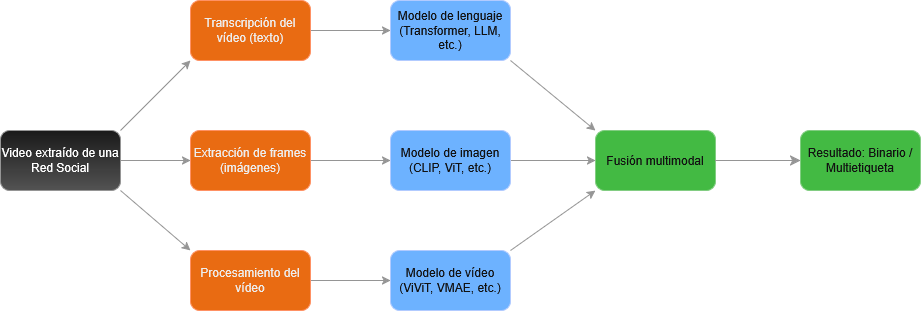
\includegraphics[width=0.9\textwidth]{Figuras/FlujoProcesamientoMultimodal.drawio.png}
    \caption{Flujo de procesamiento multimodal de vídeos (texto + imagen + vídeos)}
    \label{fig:flujo_video}
\end{figure}

Como se ilustra de manera conceptual en la \autoref{fig:flujo_video}, un flujo de procesamiento multimodal estándar divide el contenido original en sus componentes básicos. Cada modalidad es procesada de forma independiente y en paralelo por modelos específicos para extraer sus características intrínsecas. Finalmente, estas representaciones convergen en un módulo de fusión, el cual combina la información para emitir la predicción final. Este esquema teórico sirve como pilar fundamental para el diseño de arquitecturas capaces de analizar el complejo contenido multimedia actual. 

\section{Aprendizaje Profundo}
\label{sec:DeepLearning}
Dentro de la disciplina del aprendizaje automático, el aprendizaje profundo (\textit{Deep Learning}) representa una evolución significativa \cite{goodfellow2016deep}. Esta rama se fundamenta en el uso de redes neuronales artificiales, arquitecturas computacionales inspiradas en cómo el cerebro humano estructura y procesa la información. Al organizar estas neuronas artificiales en múltiples capas sucesivas, el sistema adquiere la capacidad de procesar la información de forma jerárquica, logrando un nivel de abstracción cada vez mayor. A medida que aumenta la profundidad de la red (el número de capas), el algoritmo es capaz de modelar relaciones más complejas y extraer mayor cantidad de información a partir de los datos, incluso si no es perceptible por el ser humano \cite{lecun2015deep}.

\begin{figure}[H]
    \centering
    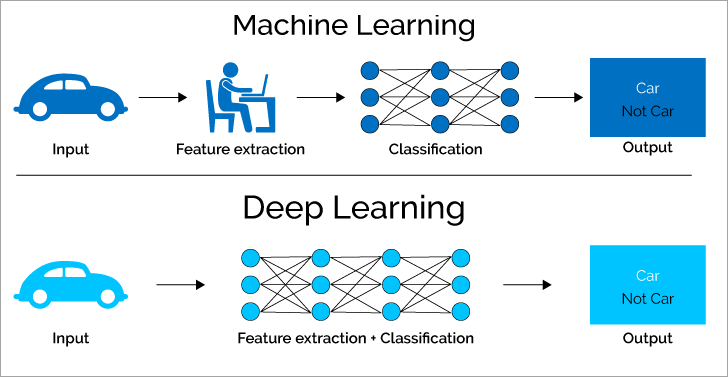
\includegraphics[width=0.9\textwidth]{Figuras/MLvsDL.png}
    \caption{Principal diferencia entre \textit{Machine} y \textit{Deep Learning}}
    \label{fig:MLvsDL}
\end{figure}

La principal diferencia entre el aprendizaje automático clásico y el aprendizaje profundo radica en el proceso de extracción de características (\textit{feature extraction}). Como se ilustra en la \autoref{fig:MLvsDL}, en los algoritmos tradicionales de \textit{Machine Learning}, es necesario que un experto humano o un proceso algorítmico previo diseñe y extraiga manualmente las características relevantes de los datos de entrada para que el clasificador pueda tomar decisiones. Por el contrario, los modelos de \textit{Deep Learning} automatizan este proceso por completo, integrando la extracción de características de forma implícita dentro de la propia arquitectura de la red. Esta capacidad de aprendizaje de extremo a extremo (\textit{end-to-end}) permite al modelo descubrir por sí mismo qué patrones son los más instructivos para resolver la tarea\cite{chollet2021deep}.

En el contexto de este Trabajo de Fin de Máster, el aprendizaje profundo constituye el núcleo técnico del sistema propuesto. Se han empleado modelos basados en arquitecturas profundas, tanto para el procesamiento de la información textual, con modelos \textit{Transformers} y Grandes Modelos de Lenguaje, como para el análisis visual, con modelos \textit{Vision Transformers}

Dado el enorme tamaño de estas arquitecturas y la complejidad matemática que entraña su ajuste, resulta indispensable comprender cómo se lleva a cabo su fase de entrenamiento. El éxito de estos modelos no depende únicamente de su estructura interna, sino de la correcta configuración de los factores que guían su aprendizaje. Por ello, en las siguientes subsecciones se detallan los hiperparámetros, mecanismos de control y conceptos fundamentales que controlan el proceso de entrenamiento. 

\subsection{Epochs y tamaño de lote}
\label{subsec:EpochsBatch}
Durante el proceso de entrenamiento de una red neuronal profunda, el modelo ajusta sus parámetros internos de forma iterativa a medida que procesa la información. El ritmo y el volumen de datos que se procesan en cada actualización de los pesos están regidos por dos hiperparámetros fundamentales de la arquitectura: la época (\textit{epoch}) y el tamaño de lote (\textit{batch size}).

Una época (\textit{epoch}) se define como un ciclo de aprendizaje completo en el que la totalidad del conjunto de datos de entrenamiento pasa a través de la red neuronal, tanto hacia adelante (\textit{forward pass}) para generar las predicciones, como hacia atrás (\textit{backward pass}) para propagar el error. Dado que los algoritmos de optimización basados en el gradiente son iterativos, una sola época rara vez es suficiente para que el modelo minimice el error adecuadamente. Por lo tanto, el entrenamiento exige realizar múltiples épocas. Sin embargo, un número excesivamente alto de épocas puede derivar en un problema de sobreajuste (\textit{overfitting}), donde el modelo comienza a memorizar los datos de entrenamiento perdiendo su capacidad de generalización \cite{prechelt2002early}.

Por otro lado, la cantidad de información que componen los conjuntos de datos actuales (especialmente aquellos con imágenes y vídeos) hace que sea computacionalmente inviable, debido a las limitaciones de memoria de las tarjetas gráficas (\textit{GPU}), procesar todos los ejemplos simultáneamente. Para solucionar esta limitación, el conjunto de entrenamiento se divide en fracciones más pequeñas denominadas lotes (\textit{batches} o \textit{minibatches}). El tamaño de lote determina el número de muestras que la red procesa antes de evaluar el error acumulado y actualizar sus pesos \cite{bengio2012practical}.

La elección del tamaño de lote tiene un impacto directo en la estabilidad y velocidad del entrenamiento. Un lote grande ofrece una estimación muy precisa del gradiente, pero requiere una enorme cantidad de memoria \textit{VRAM}. Por el contrario, un tamaño de lote pequeño introduce cierto ``ruido'' matemático en cada actualización. Curiosamente, este ruido suele ser beneficioso, ya que actúa como un mecanismo de regularización que ayuda a la red a escapar de mínimos locales y a encontrar soluciones que generalizan mejor ante datos nuevos \cite{masters2018revisiting}. 

En el contexto del ajuste fino (\textit{fine-tuning}) de arquitecturas masivas, como los \textit{Transformers} o los \textit{LLMs} empleados en este trabajo, el enorme peso de los modelos obligan a utilizar tamaños de lote muy reducidos. Asimismo, dado que estas redes ya cuentan con un amplio conocimiento adquirido durante su preentrenamiento, el número de épocas necesarias suele ser considerablemente bajo (generalmente entre 3 y 10). Un entrenamiento prolongado en estas condiciones no solo sería ineficiente, sino que podría provocar lo que se conoce como \textit{catastrophic forgetting}, el cual destruiría las representaciones lingüísticas o visuales que el modelo ya había aprendido previamente. 

\subsection{Tasa de aprendizaje y \textit{weight decay}}
\label{subsec:LearningRate}
La tasa de aprendizaje (\textit{learning rate}) es, posiblemente, el hiperparámetro más crítico en la configuración de cualquier algoritmo de optimización basado en el gradiente. Este valor determina el tamaño del paso que da el modelo en el espacio de parámetros durante cada iteración para minimizar la función de pérdida. Su correcta elección tiene un impacto significativo en la convergencia del modelo: si la tasa de aprendizaje es demasiado alta, los saltos en la actualización de los pesos serán desproporcionados, lo que puede provocar que el modelo sobrepase el mínimo óptimo y el entrenamiento se vuelva inestable. Por el contrario, si la tasa es excesivamente baja, la red tardará demasiado tiempo en converger o correrá el riesgo de quedarse estancada en un mínimo local \cite{ruder2016overview}. 

Para complementar el proceso de optimización y mitigar el riesgo de sobreajuste, es práctica común incorporar una técnica de regularización conocida como \textit{weight decay} (decaimiento de pesos). Esta técnica consiste en añadir un término de penalización a la función de pérdida que es proporcional al tamaño de los pesos de la red. De este modo, el algoritmo se ve forzado a mantener los valores de los parámetros lo más pequeños y distribuidos posible. Al evitar que unos pocos pesos adquieran valores desproporcionados, se asume que el modelo resultante es más simple y estable, lo que mejora drásticamente su capacidad para generalizar ante datos no vistos en lugar de memorizar el ruido del conjunto de entrenamiento \cite{krogh1991simple}.

En el ámbito del procesamiento del lenguaje natural y la visión por computador con arquitecturas profundas, ambos conceptos suelen trabajar de la mano mediante optimizadores avanzados como \textit{AdamW}. Al realizar el \textit{fine-tuning} de modelos masivos que ya poseen un conocimiento previo (\textit{Transformers} o \textit{LLMs}), la teoría dictamina el uso de tasas de aprendizaje muy reducidas, a menudo acompañadas de planificadores (\textit{schedulers}) que disminuyen este valor dinámicamente con el tiempo. El uso simultáneo de un \textit{learning rate} bajo y un \textit{weight decay} adecuado garantiza que el modelo se adapte a la nueva tarea de clasificación sin destruir las representaciones que adquirió durante su fase de preentrenamiento \cite{loshchilov2017decoupled}. 

\subsection{Función de pérdida}
\label{subsec:LossFunction}
Durante la fase de entrenamiento, el modelo necesita una métrica cuantitativa que evalúe la precisión de sus predicciones frente a las etiquetas reales del conjunto de datos. Esta métrica es la función de pérdida (\textit{loss function}). Su objetivo matemático es calcular el error cometido en cada predicción, devolviendo un valor que el algoritmo de optimización (mediante \textit{backpropagation}) intentará minimizar iterativamente actualizando los pesos de la red \cite{shalev2014understanding}. En los problemas de clasificación, las funciones de pérdida basadas en la teoría de la información, concretamente en el concepto de entropía, son el estándar. 

Para tareas de clasificación binaria o multiclase, donde las categorías son mutuamente excluyentes (es decir, una entrada solo puede pertenecer a una clase), se emplea la \textbf{Entropía Cruzada} (\textit{Cross-Entropy Loss}). Esta función mide la diferencia entre la distribución predicha por el modelo y la distribución real de las etiquetas. Matemáticamente, penaliza de forma logarítmica las predicciones erróneas que el modelo realiza con alta confianza, forzando al sistema no solo a acertar la clase correcta, sino a hacerlo con la mayor certeza posible \cite{murphy2012machine}. 

Por otro lado, para abordar la tarea de clasificación multietiqueta (donde un mismo registro puede presentar varias categorías de sexismo simultáneamente), el problema se descompone en múltiples clasificaciones independientes. Al tratar cada etiqueta por separado, la entropía cruzada mencionada anteriormente no es aplicable. En su lugar, se utiliza la \textbf{Entropía Cruzada Binaria} (\textit{Binary Cross-Entropy} o \textit{BCE}). Esta variante evalúa la probabilidad de presencia o ausencia de cada etiqueta de manera independiente, permitiendo que el modelo determine si una categoría específica aplica o no a la entrada, sin que dicha decisión afecte a las probabilidades del resto de etiquetas \cite{nam2014large}.

\subsection{Overfitting y técnicas de regularización}
\label{subsec:Overfitting}
Uno de los desafíos más críticos durante el entrenamiento de redes neuronales profundas es el fenómeno conocido como sobreajuste (\textit{overfitting}). Este problema ocurre cuando un modelo es excesivamente complejo en relación con la cantidad de datos de entrenamiento disponibles. En lugar de extraer patrones generales y subyacentes, la red comienza a memorizar el ruido, las anomalías y los detalles específicos del entrenamiento. Como resultado, el modelo alcanza un rendimiento excelente sobre los datos con los que ha sido entrenado, pero fracasa drásticamente al intentar generalizar y predecir sobre datos nuevos o no vistos previamente \cite{ying2019overview}.

Para mitigar el problema y forzar al modelo a aprender representaciones más robustas, se emplean diversas técnicas de regularización. Una de las estrategias más extendidas, que actúa de manera complementaria a la penalización de pesos (\textit{weight decay}) vista en apartados anteriores, es el \textit{Dropout} (abandono). 

El \textit{Dropout} es una técnica de regularización estructural que consiste en desactivar aleatoriamente una proporción de las neuronas de la red, junto con sus respectivas conexiones, durante cada iteración (\textit{forward} y \textit{backward pass}) de la fase de entrenamiento. Al ``apagar'' distintas neuronas en cada paso, se evita que las unidades de la red desarrollen una dependencia mutua excesiva. Esto obliga al modelo a distribuir el aprendizaje, garantizando que la predicción final no dependa de un pequeño grupo de neuronas fuertemente conectadas, sino del conjunto de múltiples sub-redes independientes \cite{srivastava2014dropout}.

En las arquitecturas profundas basadas en mecanismos de atención, como los \textit{Transformers} utilizados en este trabajo tanto para el procesamiento textual como visual, el \textit{Dropout} es un componente fundamental que se encuentra integrado por defecto en el diseño de sus bloques internos. La combinación del \textit{Dropout} arquitectónico con estrategias de optimización regularizadas asegura que el modelo mantenga su capacidad de generalización al adaptarse a la nueva tarea de clasificación.  

\subsection{Early stopping y validación}
\label{subsec:EarlyStopping}
Para monitorizar de forma objetiva el rendimiento de un modelo durante su fase de entrenamiento y detectar a tiempo un posible sobreajuste, resulta imprescindible el uso de un conjunto de validación. Este subconjunto de datos, que se mantiene independiente de las muestras empleadas para actualizar los pesos de la red, permite evaluar iterativamente la capacidad de generalización del modelo. Este proceso se da al finalizar cada época o tras un número determinado de iteraciones y se calcula la función de pérdida y otras métricas de rendimiento sobre este conjunto de validación. 

La observación continua de estas métricas es la base del \textit{early stopping} (parada temprana), una de las técnicas de regularización dinámica más eficaces en el aprendizaje profundo. Esta estrategia consiste en interrumpir el entrenamiento de forma automática antes de completar todas las épocas definidas si se detecta que el rendimiento en validación se estanca o empieza a degradarse, mientras que el error de entrenamiento sigue disminuyendo. Este punto de inflexión es el indicador clave de que el modelo ha dejado de aprender patrones generales y ha empezado a memorizar el conjunto de datos de entrenamiento \cite{bejani2021systematic}.

En la práctica, el \textit{early stopping} se configura mediante un parámetro conocido como paciencia (\textit{patience}), el cual define cuántas evaluaciones sin mejora se permiten antes de detener el proceso. Además de ahorrar valiosos recursos computacionales, esta técnica permite restaurar la configuración de pesos óptima (aquella que obtuvo el mejor resultado en la fase de validación) en lugar de retener los pesos deteriorados de la última época. 

Todos estos elementos analizados en las subsecciones anteriores son fundamentales para diseñar modelos robustos y reproducibles. Además, permiten explicar por qué un modelo ha funcionado mejor que otro cuando se ajustan frente a un problema complejo, más allá de lo que dictan las métricas de evaluación. Como señalan Bergstra y Bengio \cite{bergstra2012random}, el conocimiento de estos hiperparámetros y mecanismos de control es clave para mejorar la eficacia y garantizar el éxito de los modelos de aprendizaje automático.

\section{Procesamiento del Lenguaje Natural}
\label{sec:PLN}
El Procesamiento del Lenguaje Natural (PLN) es una rama de la inteligencia artificial y lingüística computacional que se ocupa de la interacción entre los sistemas informáticos y el lenguaje humano. Su objetivo principal es dotar a las máquinas de la capacidad necesaria para comprender, interpretar, generar y analizar el lenguaje natural, ya sea en formato textual o hablado. En el contexto de este Trabajo de Fin de Máster, el PLN constituye un pilar fundamental para extraer el significado y la intención de los vídeos analizados, permitiendo detectar patrones en el discurso asociados a sesgos de género, misoginia y lenguaje sexista. 

Históricamente, los sistemas de clasificación textual dependían de un preprocesamiento manual y exhaustivo. Este proceso clásico implicaba la aplicación de técnicas morfológicas para limpiar y normalizar los datos, tales como la división del texto en unidades mínimas (\textit{tokenización} por palabras), la eliminación de términos que no tienen una carga semántica dentro de la frase (\textit{stopwords}), la lematización y el truncamiento (\textit{stemming}). Tras esta fase, el texto se transformaba en matrices numéricas basadas en la frecuencia de aparición de los términos (como \textit{TF-IDF} o \textit{Bag-of-Words}). Sin embargo, estos enfoques tradicionales presentaban una limitación estructural crítica: al ignorar el orden de las palabras, se perdía gran parte del contexto y de la semántica subyacente de las frases \cite{li2022survey}.

En la actualidad, la disciplina del PLN ha experimentado una profunda evolución gracias a la adopción de nuevas arquitecturas profundas de aprendizaje automático. Los nuevos modelos, especialmente aquellos basados en la arquitectura \textit{Transformer}, han transformado el paradigma del análisis textual. En lugar de requerir una limpieza léxica manual, estos modelos utilizan tokenizadores de subpalabras (como \textit{Byte-Pair-Encoding}) y proyectan el texto en espacios vectoriales continuos de alta dimensión denominados \textit{embeddings}. Esta representación vectorial permite al modelo conservar de manera simultánea tanto la información sintáctica como la riqueza semántica. Al procesar secuencias de forma bidireccional y contextual, el sistema es capaz de captar matices lingüísticos complejos, como la ironía, el sarcasmo o el doble sentido, elementos que son intrínsecos al lenguaje natural y vitales para detectar el discurso sexista \cite{min2023recent}.

\subsection{Preprocesamiento del texto}
\label{subsec:Preprocesamiento}
Para que un modelo de aprendizaje profundo pueda procesar y extraer valor de la información textual, los datos deben someterse a una fase previa de acondicionamiento. Tal y como se ha mencionado en la sección anterior, aunque las arquitecturas basadas en \textit{Transformers} no requieren técnicas clásicas de limpieza lingüística (como la lematización), sí exigen un proceso de  eliminación de ruido específico del dominio y una tokenización matemática estricta. 

En la fase de experimentación de este trabajo, las transcripciones y textos analizados se han sometido a una tubería de limpieza (\textit{pipeline}) mediante el uso de expresiones regulares. El objetivo ha sido estandarizar el vocabulario (convirtiendo todo el texto a minúsculas) y eliminar aquellos elementos sin valor semántico que introducen ruido en la red. Concretamente, se ha procedido a la eliminación de enlaces web (\textit{URLs}), menciones a otros usuarios, etiquetas de metadatos (\textit{hashtags}), emoticonos (\textit{emojis}) y etiquetas estructurales derivadas de la transcripción de los vídeos (como los prefijos ``AUDIO:'' o ``VIDEO:''). La supresión de estos elementos resulta fundamental para aislar el discurso real y evitar que el modelo dedique recursos a aprender patrones sintácticos irrelevantes para la tarea de clasificación \cite{khurana2023natural}.

Una vez que el texto ha sido limpiado, se aplica el proceso de tokenización. Las nuevas arquitecturas emplean algoritmos de subpalabras, como \textit{Byte-Pair Encoding} (BPE) o \textit{WordPiece}. Estos enfoques son altamente eficientes, ya que conservan las palabras comunes enteras, pero dividen los términos raros, mal escritos o específicos de la jerga de internet en subunidades más pequeñas y conocidas. 

Finalmente, el tokenizador actúa como puente entre el texto y la red neuronal: toma estas subpalabras y las convierte en vectores de identificadores numéricos (\textit{input IDs}). Para garantizar que todas las secuencias adquieran una dimensión matricial uniforme antes de ser procesadas por el modelo, se aplica un proceso de truncamiento (estableciendo una longitud máxima permitida para los registros demasiado largos) y de relleno (\textit{padding}) para los textos más cortos. Adicionalmente, el tokenizador genera estructuras de control, como las máscaras de atención (\textit{attention masks}), las cuales indican al algoritmo qué partes del vector contienen información real y cuáles son simples rellenos. Este formato numérico es el único lenguaje que los modelos de aprendizaje profundo pueden procesar internamente. 

\subsection{Representación del texto}
\label{subsec:Embeddings}
Una vez que el texto ha sido tokenizado, el siguiente reto del PLN es transformar esos identificadores numéricos en un formato que capture el significado lingüístico. Históricamente, esta tarea se realizaba mediante técnicas de extracción de características basadas en frecuencias, como el \textit{Bag-of-Words} o \textit{TF-IDF}. Aunque resultan útiles en algoritmos de aprendizaje automático clásico, estas estrategias generan representaciones dispersas y asumen la independencia entre los términos, fallando a la hora de capturar las relaciones semánticas intrínsecas. 

Para superar estas limitaciones, se introdujeron los \textit{Word Embeddings} o representaciones vectoriales densas. En términos generales, un \textit{Word Embedding} proyecta cada palabra como un vector de números reales en un espacio continuo de alta dimensión, lo que permite cuantificar el contexto de una palabra, así como su similitud semántica y sintáctica, mediante distancias matemáticas.

Uno de los enfoques pioneros en este ámbito fue \textit{Word2Vec}, el cual utiliza redes neuronales poco profundas para aprender representaciones vectoriales mediante dos posibles arquitecturas: \textit{Continuous Bag-of-Words} (\textit{CBOW}), que predice una palabra objetivo a partir de su contexto, o \textit{Skip-Gram}, que realiza la tarea inversa prediciendo el contexto a partir de una palabra principal. Posteriormente, surgieron alternativas como \textit{GloVe} (\textit{Global Vectors for Word Representation}), un modelo que combina las ventajas de los métodos de ventana de contexto local con la factorización matricial global del corpus.  

Sin embargo, estos modelos estáticos presentaban una limitación estructural sin solución: el problema de la polisemia. Dado que algoritmos como \textit{Word2Vec} o \textit{GloVe} precalculan un único vector inamovible para cada término en el vocabulario, son incapaces de distinguir cuándo una misma palabra tiene significados distintos en función del contexto en la oración \cite{jurafsky2014speech}.

Esta debilidad impulsó el desarrollo de la actual generación de representaciones contextuales densas. Las nuevas arquitecturas, en lugar de consultar un diccionario estático de vectores, calculan la representación numérica de cada subpalabra de manera dinámica, analizando simultáneamente toda la secuencia que la rodea. Esta necesidad de contextualización profunda dio lugar a las arquitecturas basadas en mecanismos de atención, las cuales se abordarán en detalle en las siguientes secciones. 

\subsection{Clasificación de texto en PLN}
\label{subsec:ClasificacionPLN}
La clasificación de textos es una de las tareas computacionales más fundamentales dentro del PLN. Su objetivo principal consiste en asignar, de forma automática, una o varias categorías semánticas predefinidas a un fragmento de texto no estructurado. Dependiendo de la complejidad y la naturaleza del problema, los sistemas de clasificación se dividen en tres grandes grupos: clasificación binaria, multiclase y multietiqueta, las cuales ya fueron definidas anteriormente en el apartado \ref{sec:Clasificacion} de esta memoria.

En el contexto de este Trabajo de Fin de Máster, la clasificación de texto se emplea como motor analítico para auditar las transcripciones de los videos seleccionados. El proceso se aborda desde una doble vertiente. En primer lugar, se aplica una clasificación binaria para dictaminar si el contenido expresa algún tipo de lenguaje sexista o misógino. En caso afirmativo, el problema evoluciona hacia un esquema de clasificación más fino y detallado, cuyo objetivo es identificar qué tipos específicos de sesgos, roles de género o violencias discursivas están presentes en el mensaje. 

La relevancia de este desafío tecnológico y social queda patente en las prestigiosas campañas de evaluación competitiva organizadas por congresos internacionales como \textit{IberLEF} o \textit{CLEF}. De hecho, el marco experimental y metodológico desarrollado en este trabajo se fundamenta directamente en la competición \textit{EXIST 2025} (\textit{sEXism Identification in Social neTworks}). 

Concretamente, los modelos implementados en este proyecto dan respuesta a los retos planteados en la \textbf{Tarea 3.1} de dicha competición, centrada en la detección binaria de misoginia en redes sociales, y en la \textbf{Tarea 3.3}, enfocada en la categorización avanzada y el análisis multietiqueta del discurso machista. La participación y adaptación a este tipo de iniciativas garantiza que las soluciones aquí propuestas operan sobre un conjunto de datos estandarizado y contribuyen activamente al estado del arte en la mitigación del discurso de odio en entornos digitales. 

\section{Modelos Avanzados para Texto}
\label{sec:ModelosTexto}
La necesidad de capturar el contenido dinámico y resolver el problema de la polisemia en la representación textual ha propiciado el desarrollo de arquitecturas neuronales de última generación. En esta sección se describen los fundamentos de los modelos basados en mecanismos de atención y su evolución hasta los modernos sistema generativos, los cuales constituyen el núcleo de las tecnologías aplicadas en este trabajo. 

\subsection{Transformers}
\label{subsec:Transformers}
La arquitectura \textit{Transformer}, la cual se puede apreciar en la \autoref{fig:ArquitecturaTransformer}, supuso un cambio de paradigma en el PLN tras ser propuesta en el influyente artículo \textit{Attention is all you need} \cite{vaswani2017attention}. A diferencia de los modelos recurrentes tradicionales, como las Redes Neuronales Recurrentes (RNN) o las redes de memoria a corto-largo plazo (\textit{LSTM}), los \textit{Transformers} prescinden del procesamiento secuencial. Esta característica permite analizar las secuencias de texto en paralelo, lo que acelera drásticamente los tiempos de entrenamiento y facilita la captura de dependencias a muy largo plazo. 

\begin{figure}[H]
    \centering
    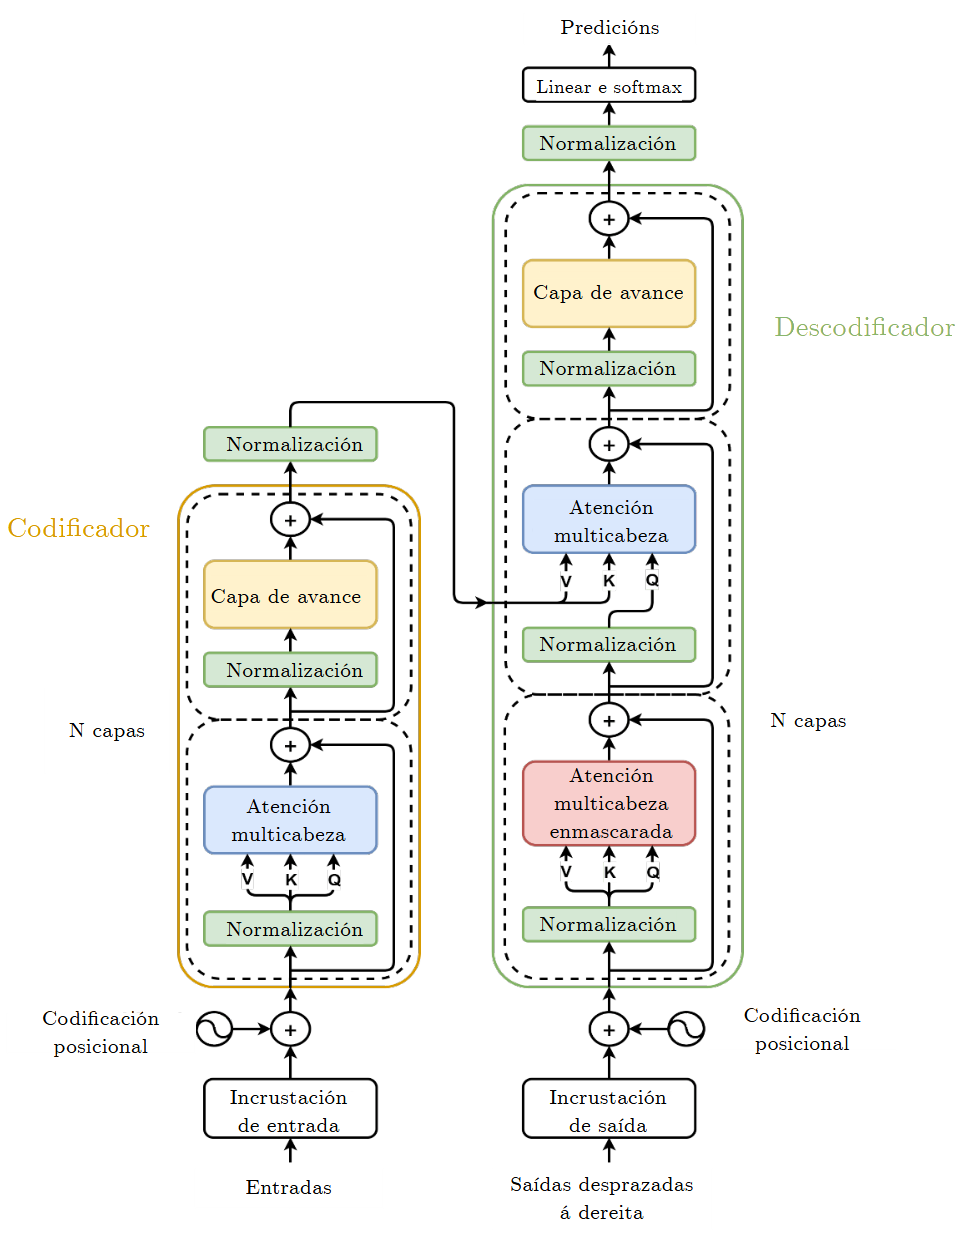
\includegraphics[width=0.9\textwidth]{Figuras/ArquitecturaTransformer.png}
    \caption{Arquitectura de los modelos \textit{Transformers}}
    \label{fig:ArquitecturaTransformer}
\end{figure}

El pilar de esta arquitectura es el mecanismo de autoatención (\textit{self-attention}), cuyo funcionamiento se ejemplifica gráficamente en la \autoref{fig:MecanismoAtencion}. Este mecanismo relaciona diferentes posiciones de una simple secuencia para computar una representación global de la misma. Matemáticamente, asigna una consulta (\textit{query}) y un conjunto de pares clave-valor (\textit{key-value}) a una salida, calculando pesos que determinan la importancia relativa de cada palabra respecto a las demás dentro de la misma oración.

\begin{figure}[H]
    \centering
    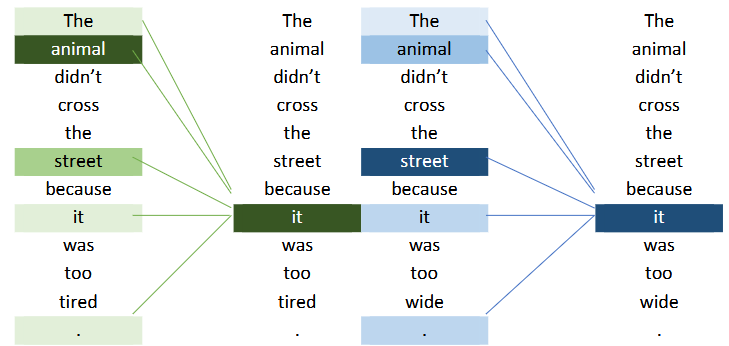
\includegraphics[width=0.9\textwidth]{Figuras/MecanismosAtencionTransformers.png}
    \caption{Ejemplo de funcionamiento del mecanismo de atención}
    \label{fig:MecanismoAtencion}
\end{figure}

Esta innovación dio lugar a una nueva generación de modelos de lenguaje preentrenados fundamentados en la codificación bidireccional, siendo \textit{BERT} (\textit{Bidirectional Encoder Representations from Transformers}) \cite{devlin2018bert} el exponente clásico. Este necesita de las entradas que se muestran en la \autoref{fig:EncoderBERT}. \textit{BERT} es capaz de aprender el contexto de una palabra observando su secuencia antecesora y predecesora de manera simultánea. Posteriormente, surgieron optimizaciones robustas como \textit{RoBERTa} (\textit{Robustly Optimized BERT Approach}) \cite{liu2019roberta}, que mejora el rendimiento eliminando la predicción de la siguiente oración durante el preentrenamiento, utilizando secuencias más largas e introduciendo un enmascaramiento dinámico de los datos. 

\begin{figure}[H]
    \centering
    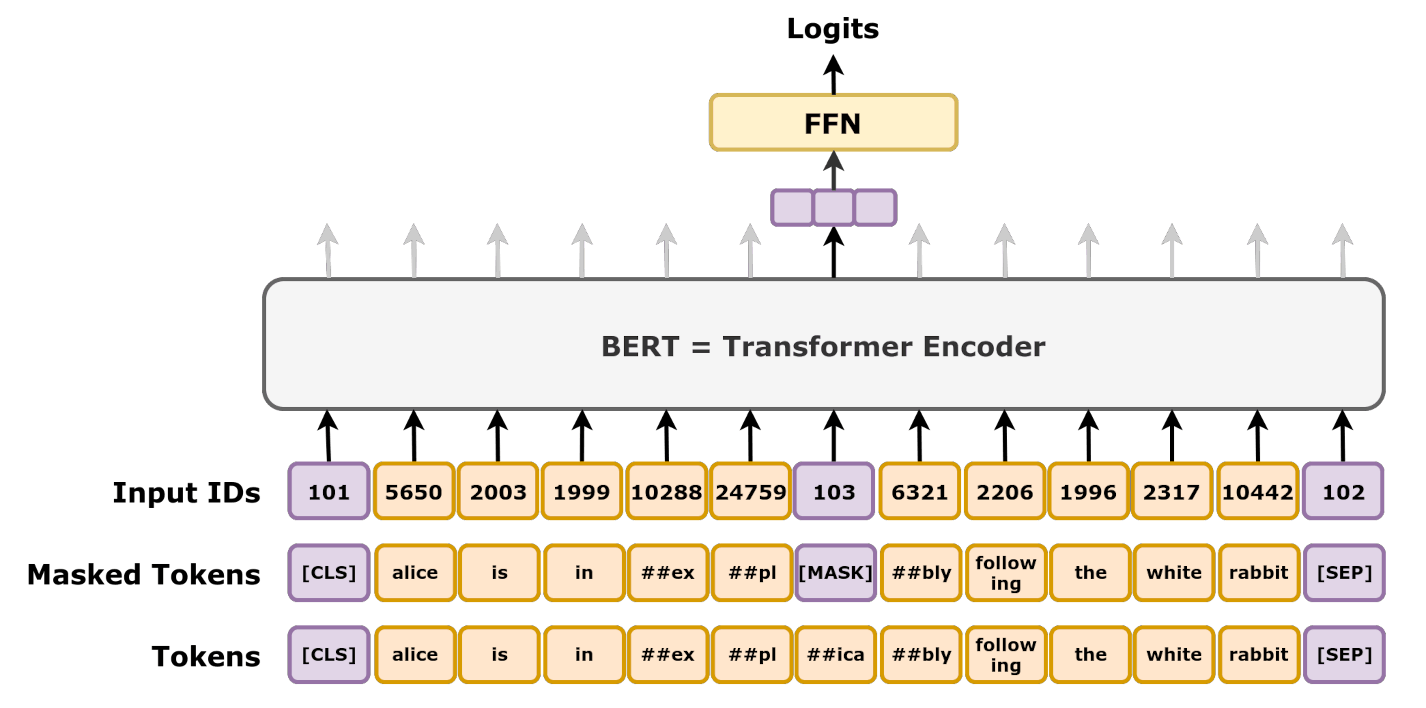
\includegraphics[width=0.9\textwidth]{Figuras/BERTEncoder.png}
    \caption{Entradas necesarias para el codificador de \textit{BERT}}
    \label{fig:EncoderBERT}
\end{figure}

\subsubsection*{Modelos implementados en este trabajo}
\label{subsubsec:ModelosTransformers}
Para abordar la complejidad de esta tarea y asegurar una evaluación exhaustiva, en el desarrollo empírico de este Trabajo de Fin de Máster se ha implementado una amplia batería de arquitecturas discriminativas basadas en \textit{Transformers}, adaptadas a diferentes dominios lingüísticos:
\begin{itemize}
    \item \textbf{Modelos Multilingües}: Se han utilizado \texttt{mmBERT}, \texttt{xlm-roberta-base} y \texttt{TwHIN-BERT}, idóneos para captar estructuras semánticas universales y transferir conocimiento entre idiomas.
    \item \textbf{Modelos específicos para Español}: Se han evaluado \texttt{BETO}, \texttt{BERTin} y \texttt{RoBERTuito}, siendo este último optimizado para el lenguaje informal de redes sociales. 
    \item \textbf{Modelos específicos para Inglés}: Se ha experimentado con \texttt{RoBERTa-Base}, \texttt{BERTweet} (preentrenado en mensajes cortos y jerga digital) y \texttt{Electra-base-discriminator} (que introduce un paradigma de reemplazo de tokens más eficiente computacionalmente). 
\end{itemize}


\subsection{Modelos Generativos de Lenguaje (\textit{LLMs})}
\label{sec:LLMs}
Paralelamente a la consolidación de modelos discriminativos como \textit{BERT}, la evolución del aprendizaje profundo ha propiciado la explosión de los Modelos Generativos de Lenguaje (\textit{Large Language Models}) \cite{zhao2023survey}. A diferencia de los enfoques anteriores, los cuales están entrenados para comprender y clasificar, los \textit{LLMs} utilizan arquitecturas autorregresivas fundamentadas habitualmente en la parte decodificadora del \textit{Transformer}. Su objetivo matemático principal es predecir el siguiente token de una secuencia para generar texto altamente coherente y contextualizado.

Modelos como \texttt{GPT-3}, \texttt{GPT-4}, \texttt{LLaMA} o \texttt{PaLM} se entrenan sobre volúmenes masivos de datos no estructurados. Gracias a este vasto conocimiento subyacente, han demostrado capacidades de generalización sorprendentes. Una de las ventajas más potentes de los \textit{LLMs} es su capacidad para ejecutar tareas supervisadas a través del diseño de instrucciones o \textit{prompting}. Existen tres estrategias principales de aplicación: 
\begin{itemize}
    \item \textbf{Zero-shot}: El modelo realiza la tarea directamente con una única instrucción, sin recibir ejemplos previos. Es idóneo cuando se busca rapidez o no se dispone de datos etiquetados. 
    \begin{itemize}
        \item \textit{Ejemplo}: ``¿La siguiente transcripción de un vídeo de TikTok a texto contiene lenguaje sexista? Texto: `Las mujeres no sirven para liderar proyectos.' Responde únicamente Sí o No''
    \end{itemize}
    \item \textbf{Few-shot}: Se incluyen varios ejemplos demostrativos dentro de la propia instrucción para que el modelo identifique el patrón deseado antes de emitir su respuesta.
    \begin{itemize}
        \item \textit{Ejemplo}:
        \begin{itemize}
            \item Texto de ejemplo: ``Todos merecemos las mismas oportunidades.'' $\rightarrow$ No sexista.
            \item Texto de ejemplo : ``Las chicas son demasiado emocionales para los negocios.'' $\rightarrow$ Sexista.
            \item Texto nuevo: ``Ellas deberían quedarse cuidando la casa.'' $\rightarrow$ El modelo infiere y dictamina que es Sexista.
        \end{itemize}
    \end{itemize}
    \item \textbf{Fine-tuning (Ajuste fino)}: Consiste en entrenar los pesos del modelo preentrenado utilizando un conjunto de datos específicos del dominio. Aunque requiere mayores recursos computacionales, suele ofrecer un rendimiento superior y constante.  
\end{itemize}

\subsubsection*{Aplicación práctica en este trabajo: \textit{PEFT} y \textit{QLoRA}}
\label{subsubsec:ModelosLLMs}
En el marco experimental de este proyecto se ha apostado firmemente por el ajuste fino. Sin embargo, debido al masivo número de parámetros de los \textit{LLMs} modernos, el reentrenamiento completo resulta computacionalmente inviable. Para solucionar este obstáculo, se ha implementado una técnica \textbf{QLoRA} (\textit{Quantized Low-Rank Adaptation}) \cite{dettmers2023qlora} sobre tres modelos generativos de última generación: \texttt{Mistral-7B-Instruct-v0.3}, \texttt{meta-llama/Llama-3.1-8B-} \texttt{Instruct} y \texttt{google/gemma-2-2b-it}. Esta metodología ha permitido cuantizar los pesos base de los modelos a una precisión de 4 bits, congelarlos, y entrenar únicamente matrices de bajo rango insertadas en las proyecciones matemáticas de atención. 

Para adaptar estos modelos a la clasificación binaria de las transcripciones de vídeo, se han desarrollado dos estrategias arquitectónicas distintas: 
\begin{itemize}
    \item \textbf{Enfoque Discriminativo (\textit{Sequence Classification})}: En los modelos \textit{Mistral} y \textit{Gemma}, se sustituyó la cabeza de modelado de lenguaje original por una capa lineal de clasificación pura (\texttt{AutoModelForSequenceClassification}), ajustando los pesos de esta nueva capa (\texttt{score}) para extraer directamente la probabilidad matemática de que el texto contenga lenguaje misógino.
    \item \textbf{Enfoque Generativo Autorregresivo (\textit{Causal LM})}: En el modelo de la familia \textit{LLaMa}, se mantuvo la arquitectura generativa intacta (\texttt{AutoModelForCausalLM}). El ajuste fino se realizó formateando las instrucciones de entrada (\textit{prompts}) para forzar al modelo a predecir y autocompletar exclusivamente un token de clasificación (``YES'' para contenido sexista o ``NO'' para contenido no sexista) mediante un optimizador supervisado (\texttt{SFTTrainer}).
\end{itemize}

\subsubsection*{Ventajas y limitaciones de la clasificación con \textit{LLMs}}
\label{subsubsec:VentajasYLimitacionesLLMs}
La adopción de estas arquitecturas masivas para tareas de clasificación del discurso de odio es una tendencia en alza, aunque presenta características contrastadas: 
\begin{itemize}
    \item \textbf{Ventajas}: Permiten aprovechar un conocimiento semántico universal y el contexto general del mundo, se adaptan rápidamente a nuevas definiciones de categorías, y alcanzan un nivel de comprensión profundo de la ironía o el sarcasmo. 
    \item \textbf{Limitaciones}: Su naturaleza generativa los hace susceptibles a sufrir alucinaciones o generar salidas inconsistentes si no se ajustan correctamente (como ocurre con la modalidad \textit{zero-shot}), exhiben una alta sensibilidad al diseño de la instrucción (\textit{prompt}) y conllevan un coste computacional elevado para inferencias masivas.
\end{itemize}

\section{Modelos Avanzados para Visión Estática (Imágenes)}
\label{sec:ModelosAvanzadosParaVisionEstatica}
De manera análoga a la evolución experimentada en el PLN, la visión por computador ha sufrido una profunda transformación en los últimos años. Una de las estrategias más eficientes para el análisis de vídeo consiste en eludir el altísimo coste computacional de las arquitecturas tridimensionales (\textit{3D-CNNs}) \cite{carreira2017quo} extrayendo secuencias de fotogramas clave y tratándolos como imágenes estáticas independientes. Para procesar estas imágenes, el estado del arte actual se divide en dos grandes enfoques según su topología.

\subsection{\textit{Vision Transformers} (\textit{ViT}) y variantes jerárquicas}
\label{subsec:ViT}
Inspirados por el abrumador éxito de los mecanismos de autoatención en el texto conseguido gracias a los \textit{Transformers}, en 2020 se introdujeron los \textit{Vision Transformers} (\textit{ViT}) \cite{dosovitskiy2020image}, demostrando que la dependencia de las redes convolucionales tradicionales no era estrictamente necesaria para tareas de visión complejas. 

La arquitectura \textit{ViT} divide la imagen original en una cuadrícula de pequeños parches (por ejemplo, 16x16 píxeles). Tal y como se muestra en la \autoref{fig:ViT} cada parche es aplanado y proyectado linealmente para formar un vector, operando funcionalmente como si fuera un \textit{token} o palabra en una frase. Tras añadir \textit{embeddings} posicionales para retener la información espacial, esta secuencia de parches se introduce directamente en el codificador de un \textit{Transformer} estándar. Al procesar las relaciones globales entre todos los parches mediante la autoatención, \textit{ViT} es capaz de captar un contexto visual integral desde las primeras capas. 

\begin{figure}[H]
    \centering
    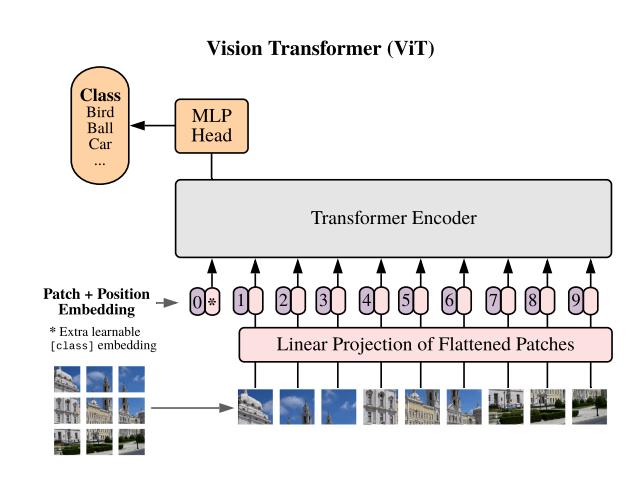
\includegraphics[width=0.9\textwidth]{Figuras/ViT.png}
    \caption{Arquitectura de un \textit{ViT}}
    \label{fig:ViT}
\end{figure}

A pesar de su éxito, \textit{ViT} presenta una complejidad computacional cuadrática respecto a la resolución de la imagen. Para solventar este problema, surgieron variantes como \textit{Swin Transformer} (\textit{Shifted Window Transformer}) \cite{liu2021swin}. Esta arquitectura jerárquica computa la atención de manera local dentro de ventanas no superpuestas que se van desplazando entre capas, lo que otorga mayor flexibilidad y eficiencia a la hora de procesar distintas escalas visuales. 

\subsection{Redes Neuronales Convolucionales Modernas (\textit{ConvNeXt})}
\label{subsec:convnext}
El auge de los \textit{ViT} llevó a repensar y modernizar el diseño clásico de las Redes Neuronales Convolucionales (\textit{CNNs}). Investigadores de \textit{Facebook} y de la Universidad de California propusieron \textit{ConvNeXt} \cite{liu2022convnet}, una arquitectura puramente convolucional construida a partir de una red residual estándar (\textit{ResNet}) \cite{he2016deep}, pero incorporando las decisiones de diseño que hicieron triunfar a los \textit{Transformers}.

Entre estas mejoras estructurales destacan el uso de tamaños de filtro (\textit{kernel}) más grandes, la sustitución de la normalización por lotes (\textit{Batch Normalization}) por la normalización de capas (\textit{Layer Normalization}), y el uso de funciones de activación más suaves. El resultado es una red que sostiene la propia eficiencia computacional de las \textit{CNNs}, pero que logra igualar o incluso superar la precisión de arquitecturas basadas en mecanismos de atención como \textit{Swin Transformer}.

\subsection{Agregación temporal para clasificación de vídeo}
\label{subsec:inferenciaViT}
Cuando estas arquitecturas de imagen estática se aplican a la clasificación de vídeos (como es el caso de este trabajo), el sistema emite una predicción matemática probabilística de forma aislada para cada fotograma extraído de la secuencia temporal. Dado que el objetivo final es emitir un único veredicto global para todo el archivo multimedia, resulta teóricamente indispensable aplicar heurísticas de agregación o \textit{pooling}.

En la literatura científica, las estrategias de consolidación más habituales para agrupar estas predicciones independientes son: 
\begin{itemize}
    \item \textbf{Max-Pooling (sensibilidad máxima)}: Consiste en evaluar el valor máximo de probabilidad de toda la secuencia. Entonces, si un solo fotograma contiene evidencias claras que superan el umbral de activación, todo el vídeo hereda dicha clasificación. Es ideal para detectar anomalías o infracciones breves pero críticas. 
    \item \textbf{Average-Pooling (Promedio continuo)}: Se calcula la media aritmética de las probabilidades de todos los fotogramas. Esta técnica exige que el contenido mantenga un nivel de confianza sostenido a lo largo del tiempo para influir en el veredicto final. 
    \item \textbf{Majority Vote (votación por mayoría)}: Cada fotograma emite un voto discreto (positivo o negativo). El vídeo adopta la clasificación que haya obtenido si supera un umbral definido previamente (lo que se consideraría como mayoría). Es una estrategia altamente robusta frente a fotogramas ruidosos, corruptos o atípicos (\textit{outliers}). 
\end{itemize}

Los detalles específicos sobre la selección de estos modelos, el volumen de fotogramas extraídos por vídeo y la implementación práctica de estas métricas de agregación se detallarán exhaustivamente en el capítulo correspondiente a la metodología experimental.  

\section{Modelos Avanzados para Visión Temporal (Vídeos)}
\label{sec:ModelosAvanzadosParaVisionTemporal}
Aunque el análisis basado en la extracción de fotogramas estáticos reduce drásticamente la carga computacional, esta metodología descarta una dimensión fundamental de los archivos multimedia: la progresión temporal. Para comprender acciones complejas, ironías o comportamientos que se desarrollan a lo largo de un clip, los sistemas de inteligencia artificial deben ser capaces de modelar conjuntamente el espacio (los píxeles en un instante dado) y el tiempo (la evolución de dichos píxeles a través de los fotogramas). En esta sección se abordan las arquitecturas modernas diseñadas para procesar el vídeo como un volumen continuo. 

\subsection{Adaptación de la Arquitectura \textit{Transformer} al Vídeo}
\label{subsec:AdaptacionDeLaArquitecturaTransformerAlVideo}
La aplicación directa del mecanismo de \textit{self-attention} a todos los píxeles de todos los fotogramas de un vídeo resulta computacionalmente inviable, ya que la complejidad matemática crece de forma cuadrática respecto a la longitud de la secuencia de entrada. Para solucionar este enorme cuello de botella, la literatura científica ha propuesto adaptaciones eficientes que extienden el éxito del \textit{ViT} al ámbito tridimensional.

\begin{figure}[H]
    \centering
    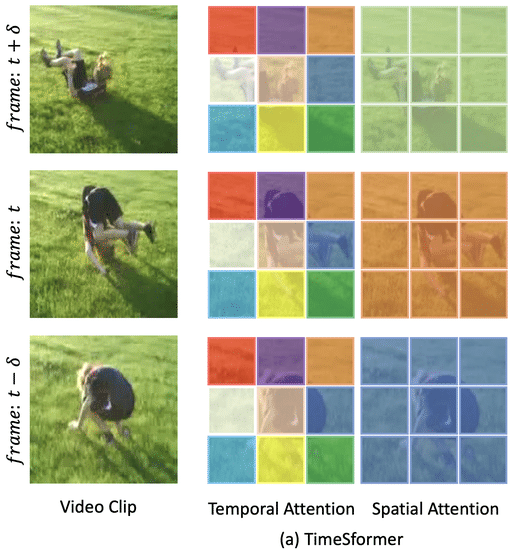
\includegraphics[width=0.6\textwidth]{Figuras/TimeSFormer.png}
    \caption{Ilustración de los mecanismos de atención de un \textit{TimeSformer}}
    \label{fig:TimeSFormer}
\end{figure}

Dentro de este campo, destacan dos enfoques arquitectónicos fundamentales implementados en el desarrollo de este trabajo: 
\begin{itemize}
    \item \textbf{\textit{TimeSformer} (\textit{Time-Space Transformer})}: Propuesto por investigadores de \textit{Facebook} \cite{bertasius2021space}, este modelo resuelve el problema de la explosión paramétrica mediante la \textbf{atención dividida}. En lugar de comparar cada parche con todos los demás parches del vídeo simultáneamente, \textit{TimeSformer} realiza el cálculo en dos pasos: primero aplica una atención puramente espacial (comparando los parches dentro de un mismo fotograma) y, a continuación, aplica una atención puramente temporal (comparando el mismo parche exclusivamente con sus homólogos en los fotogramas anteriores y posteriores), tal y como se puede observar en la \autoref{fig:TimeSFormer}. 
    \item \textbf{\textit{ViViT} (\textit{Video Vision Transformer})}: Desarrollado por investigadores de \textit{Google} \cite{arnab2021vivit}, es la evolución directa del \textit{ViT} estático. Su mayor innovación es el cambio en la forma de extraer las características iniciales: en lugar de dividir la imagen en parches bidimensionales (2D), \textit{ViViT} extrae lo que se conoce como \textbf{\textit{Tubelets}} o tubos tridimensionales. Como se puede apreciar en la \autoref{fig:ViViT}, estos tubos agrupan un bloque de píxeles que atraviesa varios fotogramas consecutivos, permitiendo a la red capturar dinámicas espaciotemporales (como la dirección y la velocidad de un movimiento) desde la primera capa del codificador.  
\end{itemize}

\begin{figure}[H]
    \centering
    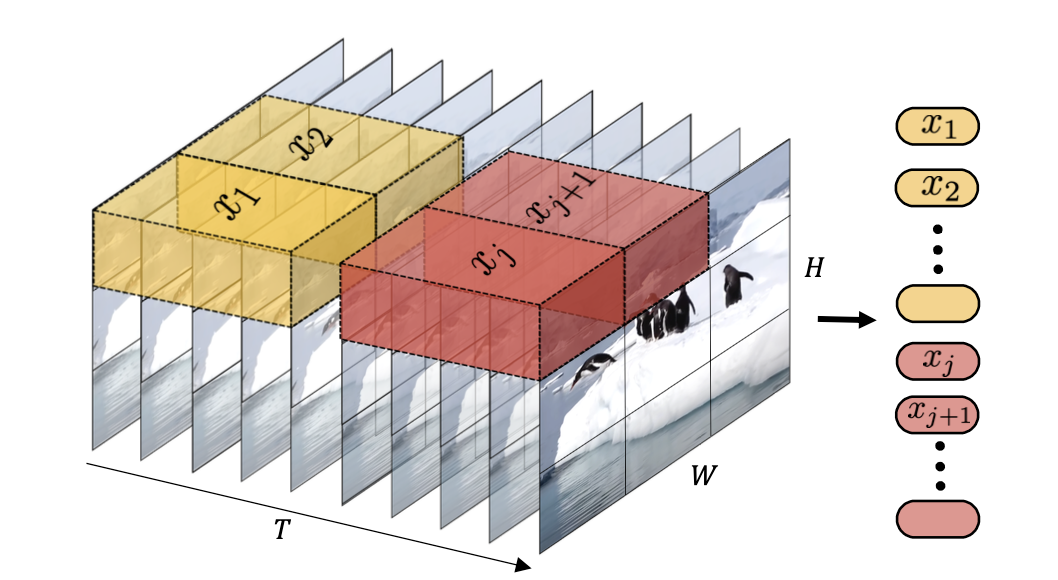
\includegraphics[width=0.9\textwidth]{Figuras/ViViT.png}
    \caption{Representación de los \textit{Tubelets} de los \textit{ViViT}}
    \label{fig:ViViT}
\end{figure}

\subsection{Enfoques Basados en Autoencoders Enmascarados}
\label{subsec:EnfoquesBasadosEnAutoencodersEnmascarados}
Paralelamente a las adaptaciones topológicas del \textit{Transformer}, el entrenamiento de modelos de vídeo ha experimentado una gran revolución gracias a las técnicas de aprendizaje autosupervisado. El principal reto del aprendizaje en vídeo es la \textbf{redundancia de la información}: dos fotogramas consecutivos suelen ser casi idénticos, lo que provoca que las redes neuronales colapsen o memoricen atajos visuales en lugar de aprender características profundas. 

Para combatir este fenómeno, surgieron modelos como \textbf{\textit{VideoMAE}} (\textit{Video Masked Autoencoders}) \cite{tong2022videomae}, una arquitectura inspirada en los métodos de entrenamiento con enmascaramiento nacidos en el PLN (como \textit{BERT}).

El funcionamiento de \textit{VideoMAE} se basa en un paradigma de reconstrucción extrema. Tal y como podemos observar en la \autoref{fig:videoMAE}, el modelo toma un volumen de vídeo (dividido en cubos espaciotemporales) y \textbf{oculta deliberadamente hasta el 90\% de la información}. El codificador (\textit{encoder}) solo procesa el 10\% de los parches visibles, y posteriormente, un decodificador (\textit{decoder}) es forzado a reconstruir todos los píxeles originales que faltan. Este nivel de enmascaramiento tan agresivo impide que la red se apoye en la redundancia temporal de los píxeles vecinos, obligándola a desarrollar una comprensión semántica de muy alto nivel sobre la física, el movimiento y la estructura de los objetos que aparecen en pantalla.

\begin{figure}[H]
    \centering
    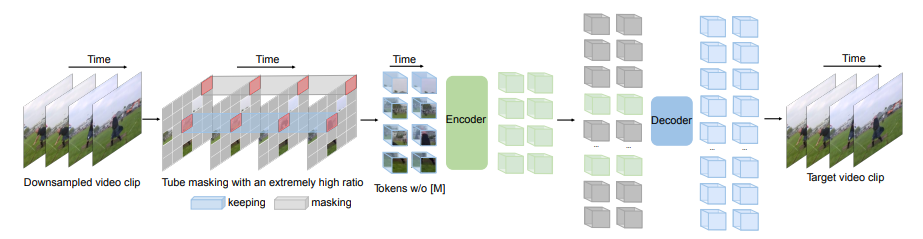
\includegraphics[width=0.9\textwidth]{Figuras/videoMAE.png}
    \caption{Arquitectura de \textit{VideoMAE}}
    \label{fig:videoMAE}
\end{figure}

\section{Aprendizaje por Transferencia}
\label{sec:TransferLearning}
El aprendizaje por transferencia (\textit{Transfer Learning}) ha revolucionado el desarrollo de la inteligencia artificial, consolidándose como el enfoque estándar en el PLN, la Visión Artificial y el aprendizaje multimodal \cite{pan2009survey}. Este paradigma consiste en reutilizar el conocimiento previamente adquirido por un modelo computacional al resolver una tarea genérica (generalmente entrenado con volúmenes de datos masivos) para aplicarlo a la resolución de una tarea nueva y específica, la cual suele disponer de una cantidad mucho menor de datos etiquetados. 

Históricamente, el desarrollo de sistemas de aprendizaje profundo exigía inicializar los pesos de las redes neuronales de forma aleatoria y entrenarlas desde cero, un proceso que requería un enorme coste computacional y bases de datos gigantescas para evitar el sobreajuste. El aprendizaje por transferencia elimina esta barrera: en lugar de aprender a extraer características desde la nada, se parte de un modelo preentrenado que ya posee representaciones universales del lenguaje (como es el caso de \textit{BERT}, \textit{RoBERTa} o \textit{GPT}) o de las imágenes \cite{qiu2020pre}. Este conocimiento base se transfiere y se refina para la nueva tarea, permitiendo democratizar el uso de modelos masivos y obtener resultados competitivos con tiempos de entrenamiento significativamente menores. 

\subsection{Fine-tuning y optimización de hiperparámetros}
\label{subsec:FineTuning}
Dentro del aprendizaje por transferencia, la estrategia de adaptación más utilizada y efectiva es el ajuste fino o \textit{fine-tuning}. Este proceso, popularizado en el PLN por enfoques como ULMFiT \cite{howard2018universal}, consiste en tomar la arquitectura de un modelo preentrenado, añadirle una nueva capa de salida orientada a la tarea específica a resolver (por ejemplo, una capa de clasificación binaria) y ajustar los pesos internos de toda la red, o de una parte de ella, utilizando un conjunto de datos propio del dominio.

Sin embargo, la literatura científica ha demostrado que modelos masivos como \textit{BERT} o \textit{RoBERTa} son altamente inestables y sensibles durante esta fase de adaptación \cite{dodge2020fine}. Para que el \textit{fine-tuning} sea exitoso y el modelo no ``olvide'' catastróficamente lo que aprendió en su preentrenamiento, resulta imprescindible realizar un proceso de \textbf{Optimización de Hiperparámetros} (\textbf{\textit{HPO}}). A nivel teórico, existen diversas estrategias para explorar el espacio de hiperparámetros: desde la búsqueda exhaustiva (\textit{Grid Search}) y la búsqueda aleatoria (\textit{Random Search}), hasta métodos avanzados como la optimización bayesiana, que modela probabilísticamente  el rendimiento de combinaciones pasadas para guiar la búsqueda de forma inteligente \cite{akiba2019optuna}.

Durante este proceso de optimización, las variables de configuración que rigen cómo aprende el algoritmo son determinantes y se dividen en:  
\begin{itemize}
    \item Por un lado, parámetros estructurales como el \textit{Learning Rate}, \textit{Weight Decay} y \textit{Epochs}, que ya fueron definidos en la \autoref{subsec:LearningRate} y \autoref{subsec:EpochsBatch} respectivamente. 
    \item Por otro lado tenemos:
    \begin{itemize}
        \item \textbf{Calentamiento (\textit{Warmup})}: Consiste en iniciar el entrenamiento con una tasa de aprendizaje cercana a cero y aumentarla gradualmente durante un porcentaje inicial de los pasos, evitando actualizaciones bruscas que desestabilicen el modelo.
        \item \textbf{Planificador de la tasa (\textit{LR Scheduler})}: Algoritmo que ajusta de forma dinámica la tasa de aprendizaje a medida que avanzan las épocas (por ejemplo, reduciéndola de forma lineal o mediante una curva coseno). 
    \end{itemize}
\end{itemize}

\subsubsection*{Estrategias avanzadas de optimización}
\label{subsubsec:EstrategiasAvanzadasDeOptimizacion}
En la práctica empírica de entrenamiento de modelos masivos como los de visión estática y los de visión temporal, la combinación de estos hiperparámetros ha dado lugar a estrategias de ajuste específicas: 
\begin{itemize}
    \item \textbf{Estrategia conservadora o \textit{Slow Cooker}}: Consiste en someter al modelo a un entrenamiento prolongado (mayor número de épocas) utilizando un \textit{learning rate} muy bajo y un \textit{weight decay} excepcionalmente alto (regularización agresiva). Se acompaña de un periodo de \textit{warmup} prolongado. Es ideal para que el modelo aprenda patrones complejos y sutilezas en conjuntos de datos difíciles sin memorizarlos. 
    \item \textbf{Simulación de lotes masivos (\textit{Gradient Accumulation})}: La memoria de las tarjetas gráficas (\textit{VRAM}) suele limitar el tamaño del lote de datos (\textit{batch size}) que se puede procesar simultáneamente. Para lograr gradientes matemáticamente estables como los que ofrecería un lote masivo, se acumulan los gradientes de varios lotes pequeños durante múltiples iteraciones antes de ejecutar la actualización de los pesos. 
    \item \textbf{Ajuste agresivo o \textit{Sprint Final}}: Se utiliza una combinación de \textit{learning rate} y regularización moderadas, pero aplicando un planificador tipo coseno (\textit{Cosine Scheduler}). Tras un calentamiento inicial, la tasa de aprendizaje se mantiene estable para luego decaer rápida y suavemente hacia el final, exprimiendo el máximo rendimiento de la red en las últimas iteraciones.
\end{itemize}

\section{Ensemble de Modelos y Fusión multimodal}
\label{sec:Ensemble}
En el ámbito del aprendizaje automático, la técnica de \textit{ensemble} (conjunto de modelos) consiste en combinar las predicciones de múltiples algoritmos diversos para generar una única decisión final más robusta, estable y precisa \cite{sagi2018ensemble}. La premisa matemática detrás de esta técnica es que, al agregar diferentes perspectivas, los errores individuales de cada modelo se compensan mutuamente, reduciendo la varianza y mitigando los sesgos específicos de cada arquitectura. 

En el contexto del análisis del discurso de odio en redes sociales, la información es inherentemente multimodal. Un vídeo no se compone de una única fuente de información, sino que abarca la transcripción textual del audio, la composición visual de sus fotogramas estáticos y la evolución temporal de sus movimientos. 

\subsection{Ventajas de los \textit{Transformers} en tareas multimodales}
\label{subsec:VentajaDeLosTransformersEnTareasMultimodales}
La capacidad de los \textit{Transformers} y de las modernas arquitecturas convolucionales para manejar secuencias de cualquier tipo y capturar dependencias a largo plazo los convierte en herramientas extremadamente potentes para tareas multimodales. En lugar de depender de un único modelo monolítico que intente comprender todo a la vez, la tendencia actual se orienta a utilizar arquitecturas expertas dedicadas que procesan el texto, la imagen y el vídeo en paralelo, combinando su información a posteriori para realizar predicciones conjuntas. Este enfoque permite capturar con una altísima precisión las relaciones y contradicciones entre lo que se dice en la transcripción de un vídeo y lo que se muestra en su componente visual. 

\subsection{Fusión Temprana vs Fusión Tardía}
\label{subsec:FusionTempranaVsFusionTardia}
A nivel teórico, la integración de múltiples modalidades de datos se divide principalmente en dos tipos \cite{baltrusaitis2018multimodal}: 
\begin{itemize}
    \item \textbf{Fusión Temprana (\textit{Early Fusion})}: Los datos o características extraídas de diferentes modalidades se combinan en las primeras etapas de la red neuronal, creando un vector unificado que es procesado por un único clasificador final. Aunque permite que el modelo aprenda interacciones cruzadas desde el principio, es computacionalmente muy costoso y propenso al \textit{overfitting} si una modalidad domina sobre las demás.
    \item \textbf{Fusión Tardía (\textit{Late Fusion})}: Cada modalidad es procesada por un modelo experto independiente hasta generar una predicción final (una probabilidad matemática). Posteriormente, estas probabilidades aisladas se combinan mediante algoritmos estadísticos para emitir el veredicto definitivo. 
\end{itemize}

En la práctica empírica y en las competiciones de Ciencia de Datos, el \textbf{\textit{late fusion} mediante predicción estática} se ha estandarizado como la metodología más eficiente. Al separar la fase de inferencia de la fase de combinación, esta técnica permite ajustar y recalcular el peso de cada modelos miles de veces en cuestión de milisegundos, sin necesidad de reprocesar repetidamente la costosa extracción de características a través de las tarjetas gráficas (\textit{VRAM}).

\subsubsection*{Promedio Ponderado (\textit{Weighted Average})}
\label{subsubsec:PromedioPonderado}
Una de las estrategias matemáticas más utilizadas en la fusión tardía es el promedio ponderado. En este método, a la probabilidad emitida por cada modelo experto se le asigna un peso específico ($w$) que refleja su nivel de fiabilidad o importancia empírica en el conjunto del sistema. Matemáticamente, la probabilidad final unificada se calcula del siguiente modo: 

\begin{equation}
    P_{final} = (w_{texto} \cdot P_{texto}) + (w_{imagen} \cdot P_{imagen}) + (w_{video} \cdot P_{video})
    \label{eq:PesosEnsemble}
\end{equation}

Sujeto a la restricción de que la suma de todos los pesos sea exactamente 1. Los valores óptimos de estos pesos no se definen arbitrariamente, sino que se descubren mediante algoritmos de búsqueda y validación cruzada que evalúan qué combinación exacta maximiza las métricas de rendimiento sobre un conjunto de datos estático. 

\section{Subjetividad en la anotación de los datos}
\label{sec:SubjetividadEnLaAnotacionDeLosDatos}
En los sistemas de aprendizaje automático tradicionales, se asume que existe una única ``verdad absoluta'' para cada conjunto de datos. Sin embargo, en tareas vinculadas al PLN que involucran un alto componente subjetivo, como la detección del discurso de odio, el sexismo o la toxicidad, esta premisa se desvanece. La percepción de un mensaje como ofensivo está intrínsecamente ligada a la sensibilidad, el contexto cultural y las experiencias vitales de la persona que lo evalúa. Por tanto, el desacuerdo entre los anotadores humanos no debe considerarse necesariamente como un ``ruido'' o un error en el conjunto de datos, sino como una señal valiosa que refleja la ambigüedad real del lenguaje humano. 

\subsection{Aprendizaje con Desacuerdo (Learning with Disagreement)}
\label{subsec:LWD}
Para gestionar esta multiplicidad de opiniones en la fase de entrenamiento de los modelos, el estado del arte ha evolucionado desde el consenso estricto hacia el \textbf{Aprendizaje con Desacuerdo} (\textit{Learning with Disagreement} o \textit{LeWiDi}) \cite{plank2022problem}. A nivel teórico, el tratamiento de las etiquetas asignadas por múltiples anotadores se aborda mediante distintas estrategias:
\begin{itemize}
    \item \textbf{\textit{Hard Labels} (Etiquetas rígidas o por Consenso)}: Consiste en fusionar las opiniones de los diferentes evaluadores en una única etiqueta definitiva. La técnica más común es el \textbf{voto por mayoría} (si dos de tres anotadores consideran un texto como sexista, la etiqueta final será positiva). En los casos donde existe un empate exacto (por ejemplo, un anotador vota a favor y otro en contra), las estrategias tradicionales optan por descartar la muestra para evitar confundir al modelo. Como alternativa, se pueden aplicar heurísticas de desempate sesgadas hacia la sensibilidad de la tarea: un enfoque pesimista (ante la duda, se cataloga como sexismo) o un enfoque optimista (ante la duda, se absuelve el comentario). 
    \item \textbf{\textit{Soft Labels} (Etiquetas Probabilísticas)}: En lugar de forzar una etiqueta binaria (0 o 1), el modelo se entrena para predecir la distribución de probabilidad de los anotadores. Si tres personas evalúan un texto y dos lo marcan como sexista, la etiqueta \textit{soft} será 0.66. Esto enseña a la red neuronal a medir el grado de polarización o ambigüedad de un mensaje. 
    \item \textbf{Desenrollado o \textit{Unrolling}}: Una estrategia de aumento de datos que evita la pérdida de información de las minorías. Consiste en duplicar el registro original tantas veces como anotadores lo hayan evaluado, asignando a cada copia la etiqueta individual de un anotador diferente. De este modo, la red neuronal se expone a todas las perspectivas humanas sin forzar un consenso matemático. 
\end{itemize}

\subsection{Perspectivismo en Inteligencia Artificial}
\label{subsec:PerspectivismoEnInteligenciaArtificial}
El perspectivismo (\textit{Data Perspectivism}) \cite{basile2021we} es una corriente reciente en la inteligencia artificial que sostiene que las características demográficas de los anotadores (como su género, edad, raza o nivel educativo) condicionan radicalmente sus respuestas. En la detección del sexismo, por ejemplo, la perspectiva de una mujer y la de un hombre frente a un mismo texto pueden diferir significativamente debido a sus vivencias estructurales. 

Para capturar y representar algorítmicamente estas visiones del mundo, la literatura propone distintas metodologías de modelado dependiendo de la naturaleza de la arquitectura utilizada: 
\begin{itemize}
    \item \textbf{Segmentación demográfica para modelos discriminativos \textit{Transformers}}: Consiste en dividir y filtrar el conjunto de datos de entrenamiento basándose exclusivamente en el perfil demográfico de los anotadores (por ejemplo, filtrando solo los votos emitidos por mujeres o solo por hombres). A partir de estos subconjuntos, se entrenan modelos discriminativos independientes. Esto da como resultado arquitecturas ``expertas'' que han interiorizado la sensibilidad y los sesgos propios de un único grupo demográfico. 
    \item \textbf{Asignación de roles para Modelos Generativos (\textit{LLMs})}: Los grandes modelos de lenguaje han interiorizado múltiples perspectivas durante su preentrenamiento masivo. Para evocar una visión demográfica específica sin necesidad de reentrenar la red, se utiliza la técnica de \textit{Persona Prompting} (ingeniería de instrucciones basada en roles) \cite{deshpande2023toxicity}. Al inyectar directrices explícitas en el \textit{prompt} del sistema (instruyendo al modelo para que ``actúe como un hombre'' o ``actúe como una mujer''), se condiciona el espacio latente de la red para que su inferencia (\textit{Zero-Shot} o \textit{Few-Shot}) adopte el sesgo cognitivo de dicho perfil demográfico. 
\end{itemize} 

\section{Medidas de Evaluación}
\label{sec:Evaluacion}
Para cuantificar de manera rigurosa y objetiva el rendimiento de los modelos desarrollados en este trabajo, se utilizan métricas estándar derivadas del aprendizaje automático. La elección de una métrica adecuada es un paso crítico en el diseño experimental, ya que no todas las medidas son igualmente válidas en todos los contextos. En tareas sensibles como la detección del discurso de odio o el sexismo, donde los conjuntos de datos suelen presentar un fuerte desbalanceo (con una presencia mayoritaria de comentarios no sexistas frente a los sexistas), basarse en métricas simples puede ofrecer una falsa sensación de eficacia algorítmica. Por ello, es necesario definir medidas específicas adaptadas a la topología de la tarea: clasificación binaria, multietiqueta o evaluación con desacuerdo. 

\subsection{\textit{Accuracy}, Precisión, Exhaustividad y \textit{F1-Score}}
\label{subsec:AccPrcExhF1s}
En las tareas de clasificación binaria (como determinar si un contenido es o no es sexista), la evaluación parte de la matriz de confusión, la cual clasifica las predicciones en Verdaderos Positivos ($TP$), Verdaderos Negativos ($TN$), Falsos Positivos ($FP$) y Falsos Negativos ($FN$). A partir de estos valores se derivan las siguientes métricas teóricas \cite{sokolova2009systematic}: 
\begin{itemize}
    \item \textbf{Exactitud (\textit{Accuracy})}: Mide el porcentaje total de predicciones correctas sobre el total de casos evaluados. Aunque es intuitiva, resulta engañosa en conjuntos de datos desbalanceados. 
    \begin{equation}
        \textit{Accuracy} = \frac{\textit{TP} + \textit{TN}}{\textit{TP} + \textit{TN} + \textit{FP} + \textit{FN}}
        \label{eq:accuracy}
    \end{equation}
    \item \textbf{Precisión (\textit{Precision})}: Evalúa la proporción de identificaciones positivas que fueron realmente correctas. Es fundamental cuando el coste de un Falso Positivo es inaceptable.
    \begin{equation}
        \textit{Precision} = \frac{\textit{TP}}{\textit{TP} + \textit{FP}}
    \label{eq:precision}
    \end{equation}
    \item \textbf{Exhaustividad (\textit{Recall})}: Mide la proporción de positivos reales que el modelo logró identificar correctamente. En la detección de discursos de odio, un alto \textit{recall} es vital para garantizar que ningún comentario dañino (Falso Negativo) pase desapercibido. 
    \begin{equation}
        \textit{Recall} = \frac{\textit{TP}}{\textit{TP} + \textit{FN}}
    \label{eq:recall}
    \end{equation}
    \item \textbf{\textit{F1-Score}}: Representa la media armónica entre la precisión y el \textit{recall}. Es la métrica estándar por excelencia en el PLN para lidiar con el desbalanceo de clases, ya que penaliza fuertemente a los modelos que favorecen una métrica a costa de destruir la otra. 
    \begin{equation}
        \textit{F1-score} = 2 \cdot \frac{\textit{Precision} \cdot \textit{Recall}}{\textit{Precision} + \textit{Recall}}
        \label{eq:f1score}
    \end{equation}
\end{itemize}

\subsection{Evaluación en clasificación multietiqueta}
\label{subsec:EvaluacionEnClasificacionMultietiqueta}
En el caso de clasificación multietiqueta (donde una misma instancia puede pertenecer a múltiples categorías simultáneamente), la evaluación matemática se vuelve más compleja. Para abordar este problema se utilizan las siguientes variantes \cite{tsoumakas2007multi}: 
\begin{itemize}
    \item \textbf{F1 Macro (\textit{Macro-F1})}: Calcula el \textit{F1-Score} de manera independiente para cada clase o etiqueta y, posteriormente, extrae la media aritmética no ponderada. Esta aproximación otorga exactamente el mismo peso a todas las clases, independientemente de su frecuencia, lo que la hace ideal para evaluar si el modelo es capaz de detectar las categorías minoritarias. 
    \begin{equation}
        \textit{Macro F1} = \frac{1}{C} \sum_{c=1}^{C} \textit{F1}_c
    \label{eq:f1macro}
    \end{equation}
    Donde $C$ es el número total de clases posibles.  
    \item \textbf{F1 Micro(\textit{Micro-F1})}: Agrega globalmente las contribuciones de todas las clases sumando los verdaderos positivos, falsos negativos y falsos positivos antes de calcular la métrica. Está fuertemente influenciada por las clases mayoritarias. 
    \item \textbf{\textit{Exact Match Ratio} (Tasa de coincidencia exacta)}: Es la métrica multietiqueta más estricta. Un acierto solo se contabiliza si el conjunto de etiquetas predichas por el modelo coincide de forma absoluta e idéntica con el conjunto de etiquetas reales de la instancia.
    \begin{equation}
        \textit{Exact Match} = \frac{1}{N} \sum_{i=1}^{N} I(Y_i = \hat{Y}_i)    
    \label{eq:exactMatchRatio}
    \end{equation} 
    Donde $I$ es la función indicadora que devuelve $1$ si los conjuntos son idénticos y $0$ en caso contrario.  
\end{itemize}

\subsection{Métricas para evaluación con desacuerdo}
\label{subsec:MetricasParaEvaluacionConDesacuerdo}
Cuando se abandona el paradigma del consenso absoluto y se entrena a los modelos utilizando \textit{Soft Labels}, las métricas tradicionales basadas en coincidencias binarias dejan de ser aplicables. En estos escenarios, el objetivo de la evaluación es medir qué tan bien se alinea la distribución de probabilidad generada por la red neuronal con la distribución real de los anotadores humanos. 

Para ello, la métrica estándar es la \textbf{Entropía Cruzada (\textit{Cross-Entropy})}, que penaliza matemáticamente las divergencias entre la predicción del modelo ($\hat{y}$) y la opinión humana real ($y$).

\begin{equation}
    CE(y, \hat{y}) = -\sum_{c=1}^{C} y_c \log(\hat{y}_c)
    \label{eq:crossEntropy}
\end{equation}

En el marco de competiciones recientes de análisis de subjetividad (como la tarea \textit{EXIST}), esta divergencia suele estandarizarse mediante la medida \textbf{\textit{ICM} (\textit{Information Contrast Measure})} \cite{plaza2023overview}. El \textit{ICM} cuantifica la calidad de la información capturada por el modelo frente a un modelo base o aleatorio. Si el modelo logra predecir con exactitud la incertidumbre y el grado de polarización de los anotadores (por ejemplo, prediciendo un 60\% de probabilidad de sexismo en un mensaje altamente debatido), el \textit{ICM} recompensa esta flexibilidad algorítmica, validando que la máquina ha comprendido la ambigüedad inherente al lenguaje natural. 

\section{Tecnologías y Recursos Utilizados}
\label{sec:Tecnologias}
El desarrollo de este proyecto se ha llevado a cabo utilizando un conjunto de herramientas y bibliotecas de código abierto ampliamente integradas en el ámbito de la inteligencia artificial, el PLN y la visión por computador. Más que una simple enumeración, estas tecnologías conforman un ecosistema cohesionado que ha permitido desde el preprocesamiento de los datos hasta el despliegue de modelos masivos.

\begin{figure}[H]
    \centering
    
\includegraphics[width=0.9\textwidth]{Figuras/TecnologiasUsadas.png}
    \caption{Tecnologías usadas para el desarrollo del TFM}
    \label{fig:tecnologiasUsadas}
\end{figure}

Como se puede observar en la \autoref{fig:tecnologiasUsadas}, las principales herramientas utilizadas han sido las siguientes: 
\begin{itemize}
    \item \textbf{\textit{Python}}: Lenguaje de programación principal de todo el proyecto, elegido por su flexibilidad, su inmenso ecosistema de librerías científicas y su estandarización absoluta en la comunidad de \textit{Data Science} y el aprendizaje automático.
    \item \textbf{\textit{Google Colab Pro} y \textit{Jupyter Notebook}}: Como entorno de desarrollo interactivo se han utilizado cuadernos de \textit{Jupyter} a través de la plataforma \textit{Google Colab}. En concreto, se ha hecho uso de recursos avanzados (aceleradores de hardware como las \textit{GPU NVIDIA L4}) para llevar a cabo el entrenamiento de modelos masivos. En total se han consumido unas 300 unidades informáticas. 
    \item \textbf{\textit{PyTorch}}: \textit{Framework} de \textit{Deep Learning} que ha servido como núcleo matemático para construir, entrenar y evaluar todos los modelos basados en \textit{Transformers} implementados en la fase empírica. 
    \item \textbf{Ecosistema \textit{Hugging Face}}: Plataforma y conjunto de bibliotecas clave en el proyecto. Se ha utilizado para importar modelos preentrenados (\textit{Mistral}, \textit{LLaMA}, \textit{Gemma}, \textit{ConvNeXt}, etc.), aplicar técnicas de \textit{PEFT} mediante inserción de matrices de bajo rango, ejecutar optimizadores supervisados como \textit{SFTTrainer}, y formatear eficientemente los conjuntos de datos.
    \item \textbf{\textit{BitsAndBytes}}: Librería fundamental de optimización de hardware que ha permitido aplicar la técnica de cuantización \textit{QLoRA}, reduciendo los pesos de los \textit{LLMs} a una precisión de 4 bits para que pudieran ser procesados en la memoria de la tarjeta gráfica disponible. 
    \item \textbf{\textit{Decord} y \textit{OpenCV} (\textit{cv2})}: Bibliotecas especializadas en el procesamiento audiovisual. Han sido fundamentales para el tratamiento de la modalidad de vídeo, permitiendo una lectura optimizada de los archivos multimedia y la extracción precisa de los fotogramas clave (\textit{frames}) requeridos por los modelos visuales. 
    \item \textbf{\textit{Scikit-Learn} y \textit{Evaluate}}: Herramientas de análisis de datos utilizadas en la fase de evaluación para computar métricas complejas de rendimiento (\textit{F1-Score}, \textit{Accuracy}, matrices de confusión) sobre los conjuntos de prueba estáticos.
    \item \textbf{\textit{Google Drive}}: Sistema de almacenamiento en la nube utilizado como repositorio de datos centralizado. Ha servido para alojar, gestionar y sincronizar todos los conjuntos de datos (\textit{datasets}), los pesos de los modelos guardados y los archivos generados durante la experimentación, permitiendo una integración y un acceso directo desde los entornos de \textit{Google Colab}.
    \item \textbf{\textit{GitHub}}: Plataforma de desarrollo colaborativo y control de versiones. Se ha empleado para estructurar de forma metódica y segura el proyecto mediante repositorios independientes: uno destinado a la centralización del código fuente y los cuadernos de experimentación \footnote{\url{https://github.com/visumania/DeepSexist}}, y otro para el control de versiones de la presente memoria \footnote{\url{https://github.com/visumania/MemoriaTFM}}. 
    \item \textbf{\textit{LaTeX}}: Sistema de composición de textos utilizado para la redacción, estructuración y maquetación de esta memoria. Su elección garantiza un formato académico riguroso, así como una gestión impecable de las referencias bibliográficas y la representación de fórmulas matemáticas. 
\end{itemize}

A modo de conclusión, en este capítulo se han establecido los fundamentos teóricos necesarios para comprender los enfoques tecnológicos implementados a lo largo del proyecto. Esta base conceptual resulta indispensable para justificar las decisiones técnicas, algorítmicas y metodológicas que se abordarán en detalle en el próximo capítulo. 
% Capítulo 3 - Metodología, Experimentación y Resultados 
\chapter{Metodología, Experimentación y Resultados}
\label{cap:Metodologia}
Este capítulo detalla el núcleo práctico y experimental del presente Trabajo de Fin de Máster. A lo largo de las siguientes secciones, se describe exhaustivamente la metodología aplicada para abordar la detección y clasificación del discurso sexista en redes sociales. En primer lugar, se contextualiza el marco del proyecto dentro del desafío de \textit{EXIST 2025}. A continuación, se expone el pipeline de preparación de los datos y se desglosan los experimentos realizados de forma unimodal (abarcando el procesamiento de texto, imágenes estáticas y secuencias de vídeo). Finalmente, se detalla la integración de estas arquitecturas mediante técnicas de fusión multimodal, culminando con un análisis profundo sobre el perspectivismo de los datos y la presentación de los resultados globales obtenidos. 

\section{Participación en el desafío \textit{EXIST 2025}}
\label{sec:ParticipacionDesafioEXIST2025}
El presente trabajo se ha desarrollado en el marco del desafío internacional \textit{EXIST 2025} (\textit{sEXism Identification in Social neTworks}). Esta iniciativa tiene como objetivo principal pedir a los participantes que identifiquen y caractericen el sexismo en las redes sociales. Su propósito fundamental es ayudar a identificar tendencias y patrones de comportamiento sexista en diversos formatos multimedia y de interacción de usuarios, contribuyendo así a una comprensión más profunda de estas dinámicas sociales y a su potencial aplicabilidad en sistemas de moderación de contenido. 

\subsection*{Estructura del reto y modalidades}
\label{subsec:EstructuraDelRetoYModalidades}
En su edición de 2025, la organización ha dado un salto cualitativo hacia la multimodalidad, conformando un total de nueve subtareas disponibles en dos idiomas (inglés y español). Estas subtareas se estructuran en torno a tres ejes principales (Identificación de sexismo, Detección de la intención de la fuente y Categorización del sexismo) aplicadas a tres tipos de datos diferentes:
\begin{itemize}
    \item \textbf{Tarea 1 (Texto)}: Centrada en el análisis de \textit{tweets}.
    \item \textbf{Tarea 2 (Imágenes)}: Enfocada en la evaluación de memes, extrayendo su información visual y textual mediante \textit{OCR}.
    \item \textbf{Tarea 3 (Vídeos)}: Basada en archivos multimedia extraídos de la plataforma \textit{TikTok}.
\end{itemize}

Esta aproximación multimodal resulta esencial para evaluar la capacidad real de los sistemas a la hora de detectar la subjetividad y la ofensa en fuentes de datos complejas.

\subsection*{Participación global y datos del reto}
\label{subsec:ParticipacionGlobalYDatosDelReto}
La relevancia de esta edición quedó demostrada por un nivel de implicación excepcional en la comunidad científica. Un total de 244 equipos de 38 países se registraron en \textit{EXIST 2025}, de los cuales 114 (procedentes de 23 países) lograron enviar al menos una entrega (\textit{run}) oficial. En conjunto, se recibieron 873 envíos, de los cuales 589 se evaluaron mediante \textit{Hard-labels} y 284 mediante \textit{Soft-labels}.

Aunque la mayoría de los participantes concentraron sus esfuerzos en el análisis puramente textual de la Tarea 1 (596 envíos evaluados), la Tarea 3 dedicada al análisis de vídeo atrajo un interés significativo con 211 envíos, lo que subraya la creciente relevancia de los enfoques multimodales en el PLN. 

\subsection*{Nuestras entregas oficiales y motivación del TFM}
\label{subsec:NuestrasEntregasOficialesYMotivacionDelTFM}
En el contexto oficial del desafío, la participación de nuestro equipo (\textit{I2C-UHU}) se enmarcó dentro de la Tarea 3 de vídeos, concretamente en la \textbf{Subtarea 3.1 (Identificación de Sexismo)}. Se trata de un problema de clasificación binaria donde el sistema debe decidir si un contenido dado refleja expresiones o comportamientos sexistas, clasificándolo bajo las categorías ``YES'' o ``NO''.

Para nuestras dos entregas oficiales, se optó por un enfoque inicial unimodal, evaluando la capacidad de la transcripción textual del vídeo para resolver la tarea. Se realizaron los siguientes envíos bajo la evaluación \textit{Hard}:
\begin{enumerate}
    \item \textbf{I2C-UHU-Sirius\_1}: Un modelo discriminativo de la familia \textit{Transformer} (\texttt{bert} \texttt{-base-multilingual-cased}), ajustado mediante \textit{fine-tuning} para la clasificación de secuencias.
    \item \textbf{I2C-UHU-Sirius\_2}: Un \textit{LLM} generativo (\texttt{meta-llama/Llama-3.2-1B-Instruct}), evaluado bajo un enfoque \textit{Zero-Shot} mediante técnicas de \textit{Prompt Engineering}.  
\end{enumerate}

En la \autoref{tab:ResultadosOficialesEXIST} se detallan las métricas oficiales obtenidas por nuestros sistemas en la evaluación oficial sobre un total de 43 participaciones admitidas en la tabla de clasificación (\textit{leaderboard}) para esta subtarea. Cabe destacar que estas métricas oficiales basadas en \textit{ICM-Hard} y el \textit{F1} de la clase \textit{YES} responden a un protocolo específico (el definido por la organización) y no son directamente comparables con los resultados locales obtenidos en fases posteriores de este trabajo (medidos habitualmente mediante \textit{macro-F1}).

\begin{table}[H]
    \centering
    \begin{tabular}{lcccc}
        \toprule
        \textbf{Envío Oficial} & \textbf{Ranking} & \textbf{ICM-Hard} & \textbf{ICM-Hard Norm} & \textbf{F1 Macro} \\
        \midrule
        (\textit{BERT}) & 31 & -0.1278 & 0.4355 & 0.5768 \\
        (\textit{LLaMA}) & 39 & -0.4212 & 0.2874 & 0.1379 \\
        \bottomrule
    \end{tabular}
    \caption{Resultados oficiales obtenidos en la Subtarea 3.1 de EXIST 2025}
    \label{tab:ResultadosOficialesEXIST}
\end{table}

Lejos de ser el objetivo final de esta investigación, la participación en el desafío y los resultados expuestos actuaron como el \textbf{\textit{baseline}} de este Trabajo de Fin de Máster. Las métricas alcanzadas (en especial el bajo rendimiento del enfoque \textit{Zero-Shot}) permiten plantear la hipótesis de que la restricción metodológica a un formato exclusivamente textual (sumada a factores simultáneos como el tamaño del modelo, el diseño del \textit{prompt}, la ausencia de ajuste fino y la naturaleza específica del conjunto de validación) pudo influir en los resultados. Esta comprobación preliminar sirvió de base para motivar y justificar el posterior trabajo empírico, desarrollado en esta memoria: la extracción de fotogramas, la experimentación profunda con modelos de visión estática y temporal, la integración mediante \textit{Ensembles} y el análisis de la subjetividad de los anotadores.

\section{Descripción General de la Metodología}
\label{sec:Metodologia}

\begin{figure}[H]
    \centering
    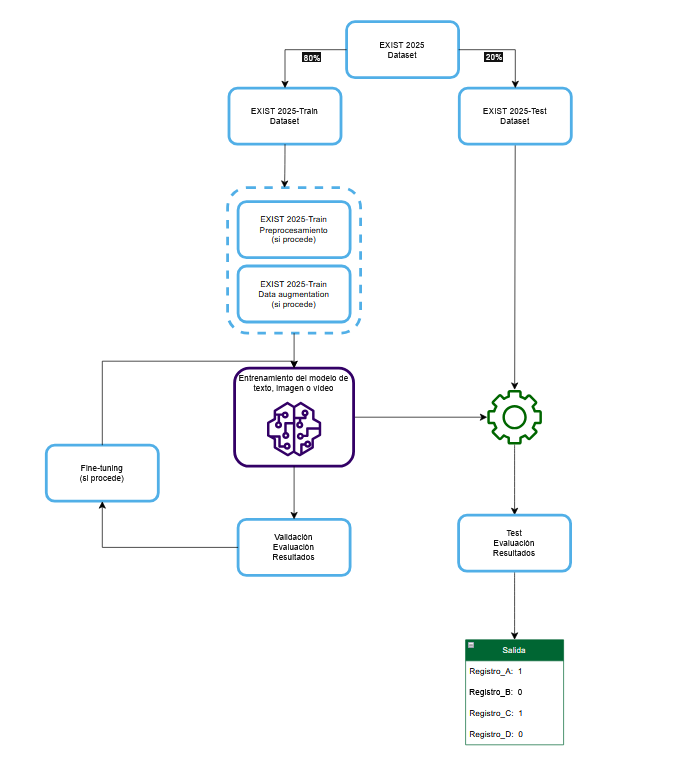
\includegraphics[width=0.9\textwidth]{Figuras/PipelineSeguida.png}
    \caption{Pipeline general del marco de experimentación}
    \label{fig:PipelineSeguida}
\end{figure}

El marco de experimentación diseñado para este Trabajo de Fin de Máster se ha dividido en un flujo de trabajo iterativo e incremental: comenzando por el preprocesamiento de los datos, pasando por el diseño y entrenamiento de modelos unimodales, y culminando con la fusión multimodal y la evaluación del rendimiento bajo diferentes perspectivas. En esta sección se ofrece una visión general del proceso completo, el cual será detallado en profundidad en secciones posteriores. 

La \autoref{fig:PipelineSeguida} muestra el \textit{pipeline} del marco de experimentación seguido en este trabajo. 

De forma estructurada, la secuencia completa de procesos abordada para resolver la detección y categorización del discurso sexista se divide en las siguientes fases principales:
\begin{enumerate}
    \item \textbf{Preparación y Tratamiento de Datos}: Esta fase inicial engloba la limpieza del corpus textual y la estandarización del conjunto de datos mediante una división estratificada. Se generó un conjunto de \textit{Train} y un \textit{Test} local de desarrollo (destinado empíricamente a la calibración y selección de modelos). Para garantizar una reproducibilidad estricta, los identificadores exactos (\textit{IDs}) de los vídeos pertenecientes a cada partición se han publicado en el repositorio del proyecto. Finalmente, se llevó a cabo la extracción automatizada de características visuales, procesando los archivos multimedia para generar diferentes conjuntos de \textit{frames}.
    \item \textbf{Selección y Entrenamiento Unimodal}: Ante la complejidad del formato vídeo, se optó por la estrategia de ``divide y vencerás'', seleccionando y entrenando arquitecturas expertas para cada modalidad de forma aislada:
    \begin{itemize}
        \item \textit{Modalidad de texto}: Experimentación con modelos discriminativos multilingües (familia \textit{Transformer}) y modelos generativos masivos (\textit{LLMs}).
        \item \textit{Modalidad de Visión Estática y Temporal}: Ajuste de modelos convolucionales de imágenes y redes especializadas en vídeo para captar el contexto visual del problema.
    \end{itemize}
    \item \textbf{Ajuste de Hiperparámetros}: Proceso crítico aplicado a los mejores modelos base seleccionados en la fase anterior. Implicó la exploración del espacio de hiperparámetros (\textit{learning rate}, \textit{weight decay}, \textit{warmup}) para lograr un \textit{fine-tuning} estable, evitando el olvido catastrófico del conocimiento previo de las redes. 
    \item \textbf{Fusión Multimodal (\textit{Ensemble})}: Etapa de consolidación donde las predicciones aisladas de los modelos de texto, imagen y vídeo se combinaron en un único sistema robusto mediante una estrategia de \textit{Late Fusion}, optimizando matemáticamente los pesos de cada modalidad para la Tarea 3.1.
    \item \textbf{Perspectivismo y Análisis de Errores}: Aprovechando el \textit{LeWiDi} del conjunto de datos original, se volvieron a entrenar las mejores arquitecturas de la modalidad de texto segmentando los datos en función del género de los anotadores (perspectiva de hombres frente a mujeres) y se inyectaron roles en los \textit{LLMs} mediante \textit{Persona Prompting} para analizar la subjetividad de los fallos del sistema.  
    \item \textbf{Evaluación y Experimentación Multietiqueta}: Fase final orientada a cuantificar el rendimiento mediante métricas estándar sobre los conjuntos estáticos y a adaptar los mejores modelos unimodales para resolver el problema secundario de la Tarea 3.3 (clasificación independiente de las distintas categorías del sexismo). 
\end{enumerate}

\section{Preparación de los Datos}
\label{Preparacion_Datos}
El rendimiento de los modelos de \textit{deep learning} depende de la calidad y el formato de los datos con los que son entrenados. Por ello, antes de proceder a la fase de modelado, se diseñó un riguroso \textit{pipeline} de preparación. Esta sección detalla la exploración inicial del conjunto proporcionado, la resolución de conflictos con las etiquetas, el preprocesado de las transcripciones textuales y la extracción estructurada de las características visuales a partir de los vídeos originales. 

\subsection{Descripción del Conjunto de Datos y División (\textit{Train} y \textit{Test})}
\label{DescripciónDelConjuntoDeDatosYDivisionTrainYTest}
\begin{figure}[H]
    \centering
    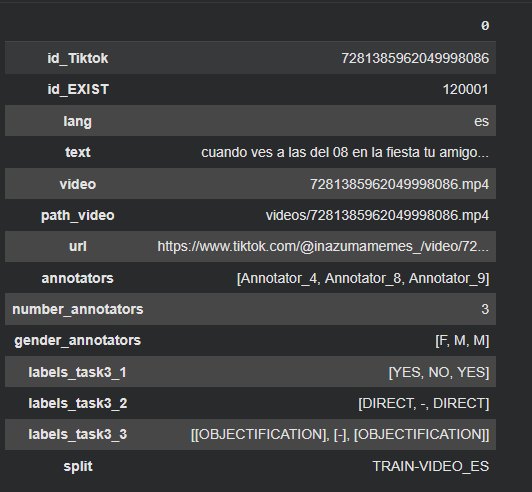
\includegraphics[width=0.9\textwidth]{Figuras/DatasetOriginal.png}
    \caption{Ejemplo de un registro del dataset original}
    \label{fig:DatasetOriginal}
\end{figure}

El conjunto de datos original proporcionado por la organización para la Tarea 3 estaba compuesto por 2524 vídeos extraídos de la plataforma \textit{TikTok} (1524 en español y 1000 en inglés). Estos datos se encontraban estructurados en un archivo \textit{JSON} donde los campos más relevantes para nuestra tarea eran el identificador (\texttt{id\_EXIST}), el texto (\texttt{text}), la ruta del archivo (\texttt{path\_video}), el recuento de los anotadores (\texttt{number\_annotators}) y la lista de valoraciones (\texttt{labels\_task3\_1}). Al basarse en el paradigma de \textit{LeWiDi}, los vídeos no contaban con una etiqueta única, sino que presentaban las decisiones individuales de 2 o 3 anotadores distintos, tal y como se puede observar en la \autoref{fig:DatasetOriginal}.

Para adaptar este conjunto a los requisitos de la Tarea 3.1 (clasificación binaria \textit{Hard} en ``YES'' o ``NO'') era necesario fusionar las múltiples opiniones en una única etiqueta. Según la documentación oficial del reto, el proceso de anotación contemplaba la participación de dos anotadores independientes y la intervención de un investigador experto para adjudicar y resolver los casos de desacuerdo. Al explorar el campo \texttt{labels\_task3\_1}, se verificó que la presencia de un tercer voto correspondía a la inclusión de este veredicto de desempate. 

Dado que el archivo en bruto proporcionado no exponía de forma explícita una columna con la etiqueta \textit{Gold Standard} unificada, se optó por ignorar el supuesto \textit{label} oficial externo y reconstruir las etiquetas desde las matrices de votación para asegurar la coherencia absoluta del conjunto de entrenamiento:
\begin{itemize}
    \item \textbf{Voto por mayoría}: En la inmensa mayoría de las instancias, que contaban con 3 anotadores (reflejando la adjudicación),se asignó directamente la etiqueta mayoritaria. Por ejemplo: un registro con los votos \texttt{[YES, NO, YES]} se catalogó de forma automática como sexista.
    \item \textbf{Descarte por conflicto}: Durante el procesamiento de las etiquetas, se aplicó un \textbf{criterio} estricto de exclusión para aquellos casos en los que no se llegó a un consenso. Específicamente, se detectaron 16 casos residuales evaluados únicamente por 2 anotadores en los que existía un empate absoluto (1 voto a favor y 1 en contra), sin constancia de un tercer voto de resolución en la matriz de datos. En lugar de forzar una asignación de manera manual o aleatoria, se eliminaron estas muestras. El \textbf{impacto} estadístico de esta decisión supone una reducción marginal del corpus (eliminando apenas un 0.8\% de los datos, para fijar el conjunto final de entrenamiento en 2006 instancias), pero resulta metodológicamente crítico para evitar inyectar ruido e inconsistencias en la red neuronal. Para garantizar la trazabilidad de esta limpieza, los identificadores de estas muestras han sido documentados \footnote{Los \textit{IDs} de los 16 vídeos descartados por empate absoluto son: [120157, 120165, 120478, 120551, 120785, 120997, 121304, 121316, 220023, 220157, 220778, 220793, 220872, 220921, 220929, 121443]}.

\end{itemize}

Para asegurar la total reproducibilidad de esta reducción, el filtro se ejecutó automáticamente mediante un \textit{script} incluido en el cuaderno \texttt{Dataset\_Task\_3\_1.ipynb}. Tras aplicarlo, tal y como se puede apreciar en la \autoref{fig:Dataset3.1Transformado}, el conjunto original de 2524 vídeos se redujo a 2508 registros limpios (1306 no sexistas y 1202 sexistas), garantizando que los modelos se entrenaran exclusivamente sobre instancias con un consenso humano verificable.  

\begin{figure}[H]
    \centering
    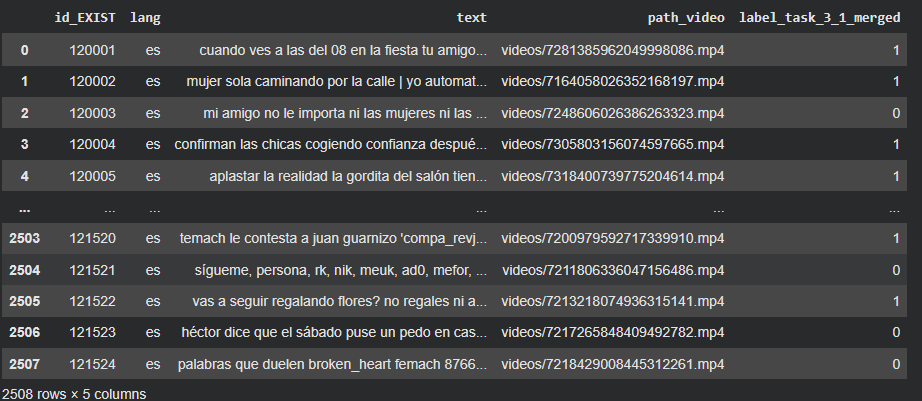
\includegraphics[width=0.9\textwidth]{Figuras/Dataset3.1Transformado.png}
    \caption{Dataset transformado para la tarea 3.1}
    \label{fig:Dataset3.1Transformado}
\end{figure}

Posteriormente, el conjunto consolidado se dividió en dos subconjuntos manteniendo una proporción del 80\% para \textit{Train} y un 20\% para \textit{Test} de validación interna. Se utilizó una técnica de muestreo estratificado (\textit{stratify}) para asegurar que la proporción de clases se mantuviera idéntica en ambos bloques, fijando una semilla aleatoria (\texttt{random\_state=42}) para garantizar la reproducibilidad de la partición. Como se puede observar en la \autoref{tab:distribucionesFichero3.1}, el conjunto de \textit{Train} final quedó conformado por 2006 instancias (1045 negativas, 961 positivas), mientras que el conjunto de \textit{Test} local constó de 502 instancias (261 negativas, 241 positivas). 

Cabe reconocer que esta metodología no reproduce el protocolo empleado por la organización para generar el \textit{Test} ciego oficial, el cual está fundamentado en una partición cronológica y agrupada por autor para evitar sesgos. Por consiguiente, nuestro marco de calibración local asume un riesgo potencial de fuga de información (\textit{data leakage}), ya que vídeos de un mismo autor de \textit{TikTok} podrían quedar repartidos entre entrenamiento y validación. Esto remarca el carácter exploratorio de nuestras métricas locales, haciendo indispensable la evaluación final sobre el entorno de desafío para confirmar la viabilidad del sistema. 

\begin{table}[H]
    \centering
    \begin{tabular}{lccc}
        \toprule
        \textbf{Fichero} & \textbf{Train} & \textbf{Test}\\
        \midrule
        Etiqueta 1 & 961 & 241 \\
        Etiqueta 0 & 1045 & 261 \\
        Total & 2006 & 502 \\
        \bottomrule
    \end{tabular}
    \caption{Distribuciones del fichero \text{Train} y \textit{Test} para la tarea 3.1}
    \label{tab:distribucionesFichero3.1}
\end{table}

\subsection{Preprocesado de texto, limpieza y tokenización}
\label{PreprocesadoDeTextoLimpiezaYTokenizacion}
Las transcripciones automáticas de los vídeos suelen presentar irregularidades gramaticales. Por ello, el \textit{pipeline} de limpieza se diseñó para operar directamente sobre el campo \textit{text} unificando el tratamiento para ambos idiomas (español e inglés). Primero, el texto fue estandarizado transformando los valores nulos y forzando la compatibilidad de tipo \textit{string} para evitar fallos de ejecución. A continuación, tal y como se describió en el marco teórico, se aplicó una tubería secuencial basada en la librería nativa de expresiones regulares (\textit{regex}), siguiendo este orden de ejecución:

\begin{enumerate}
    \item \textbf{Normalización base}: Conversión de toda la cadena de texto a caracteres en minúsculas.
    \item \textbf{Estructuras de transcripción}: Eliminación de prefijos originados por el sistema de captura del reto (ej. borrado literal de los patrones \texttt{``AUDIO:''} y \texttt{``VIDEO:''}).
    \item \textbf{Metadatos web}: Búsqueda y eliminación de enlaces externos (\textit{URLs}).
    \item \textbf{Interacciones sociales}: Supresión de menciones directas a otros usuarios de la red social (patrón \texttt{@usuario}) y limpieza de etiquetas (\textit{hashtags}).
    \item \textbf{Símbolos y ruido}: Borrado de emoticonos (\textit{emojis}), caracteres especiales y puntuaciones atípicas que no aportan significado semántico al clasificador.
\end{enumerate}

Una vez finalizada la limpieza del texto, el proceso de tokenización varió drásticamente en función de la familia de modelos utilizados: 
\begin{itemize}
    \item \textbf{\textit{Transformers}}: Se emplearon los tokenizadores nativos de cada arquitectura (utilizando algoritmos como \textit{WordPiece} para las variantes de \textit{BERT} y \textit{Byte-Pair Encoding} o \textit{BPE} para \textit{RoBERTa}). Para garantizar la uniformidad de los tensores de entrada y optimizar el consumo de memoria de la GPU, se aplicó un truncamiento y rellenado dinámico (\textit{padding}) estableciendo una longitud máxima de secuencia (\textit{max\_length}) de \textbf{[128]} \textit{tokens}. A nivel interno, una frase como ``\textit{El machismo no existe}'' se descompone en tokens elementales y se traduce a un vector numérico estructurado (por ejemplo: \texttt{[101, 235, 14234, 156, ...]}) denominado \texttt{input\_ids}, acompañado de una máscara de atención (\texttt{attention\_mask}).
    \item \textbf{\textit{LLMs}}: Para el \textit{fine-tuning} de modelos como \textit{LLaMA} o \textit{Mistral}, el preprocesamiento exigió la implementación de una técnica de \textit{Prompt Engineering}. Cada transcripción se envolvió en una plantilla estructurada que indicaba explícitamente al modelo su tarea, restringiendo su vocabulario de salida exclusivamente a las palabras ``YES'' o ``NO''.
\end{itemize}

\subsection{Extracción de Características Visuales}
\label{subsec:ExtraccionDeCaracteristicasVisuales}
Para que los modelos de visión por computador pudieran analizar el contenido de \textit{TikTok}, fue necesario transformar los archivos temporales de vídeo (.mp4) en fotogramas estáticos legibles por redes convolucionales. Este proceso se llevó a cabo utilizando la biblioteca de visión artificial \textit{OpenCV}.

Es importante resaltar que la separación de los datos en los subconjuntos \textit{Train} y \textit{Test} descrita en la primera subsección se realizó aislando el identificador único del vídeo \texttt{id\_EXIST} de manera completamente previa a la extracción de imágenes. El script de procesamiento de \textit{frames} operó leyendo de forma aislada los ficheros que ya estaban particionados. Esta metodología actúa como una estrategia robusta de \textit{GroupSplit}, asegurando que no exista fuga de datos (\textit{data leakage}): todos los datos extraídos de un mismo vídeo recaen íntegramente en la misma partición, impidiendo que el modelo sea evaluado con escenas que ya memorizó durante el entrenamiento. 

Con el objetivo de explorar la cantidad óptima de información visual requerida, se construyeron múltiples \textit{datasets} extrayendo un número variable de fotogramas por vídeo: $N \in \{2, 4, 6, 8, 10\}$. En la \autoref{tab:TamañosFicherosFrames} se aprecian los tamaños y distribuciones de los nuevos \textit{corpus} de imagen generados. Para garantizar que las capturas fueran verdaderamente representativas del contenido global y evitar \textit{frames} en negro al inicio o al final del vídeo, se diseñó un algoritmo de muestreo equidistante. La frecuencia o paso de extracción (\textit{step}) se calculó matemáticamente mediante la siguiente ecuación:

\begin{equation}
    step = \left\lfloor \frac{\text{total\_frames}}{N + 1} \right\rfloor
\end{equation}

\begin{table}[H]
    \centering
    \begin{tabular}{lccc}
        \toprule
        \textbf{Fichero} & \textbf{Train} & \textbf{Test}\\
        \midrule
        Original & 2006 & 502 \\
        2 \textit{Frames} & 4012 & 1004 \\
        4 \textit{Frames} & 8024 & 2008 \\
        6 \textit{Frames} & 12036 & 3012 \\
        8 \textit{Frames} & 16048 & 4016 \\
        10 \textit{Frames} & 20060 & 5020 \\

        \bottomrule
    \end{tabular}
    \caption{Tamaños de los ficheros \text{Train} y \textit{Test} en función de los \textit{frames} extraídos}
    \label{tab:TamañosFicherosFrames}
\end{table}

Posteriormente, las imágenes extraídas se almacenaron en formato \textit{JPG} y se indexaron en un nuevo fichero tabular, heredando la etiqueta binaria de su vídeo original, lo que permitió el entrenamiento supervisado de las arquitecturas de imagen.

\section{Experimentación Unimodal en Texto}
\label{sec:ExperimentacionUnimodalEnTexto}
La primera fase de la metodología empírica se centró de manera exclusiva en el procesamiento de la modalidad textual. Las transcripciones de los vídeos de \textit{TikTok} que se nos aportaron en el \textit{dataset} por parte de los organizadores poseen una alta densidad de información, ya que la mayor carga semántica e ideológica del discurso sexista suele residir en el lenguaje verbal. Para abordar esta tarea, se dividió la experimentación en dos vertientes del PLN: el uso de arquitecturas discriminativas clásicas y la implementación de Grandes Modelos de Lenguaje (\textit{LLMs}) generativos. 

En todos los experimentos de esta fase, se partió del conjunto maestro de entrenamiento (2006 instancias), el cual fue subdividido internamente en un 90\% para \textit{Train} (1805 instancias) y un 10\% para \textit{Validation} (201 instancias), fijando la semilla aleatoria para garantizar un marco comparativo justo entre arquitecturas. 

\subsection*{Entorno de Experimentación y Limitaciones}
Para asegurar la reproducibilidad de los resultados presentados, es fundamental detallar el entorno técnico. Todos los experimentos se ejecutaron sobre una \textit{GPU NVIDIA L4} con 23.66 GB de \textit{VRAM}, utilizando el marco de trabajo de \textit{PyTorch}, \textit{PyTorch Lightning} y la librería \textit{Transformers}.

Debido a las estrictas limitaciones computacionales y de tiempo operativo derivadas del procesamiento profundo en redes neuronales, cada configuración se ejecutó una única vez. Esta metodología constituye una limitación formal del estudio: al carecer de ejecuciones múltiples, las variaciones en el rendimiento entre ciertos modelos podrían atribuirse a la aleatoriedad de la inicialización de los pesos y no únicamente a la superioridad de una arquitectura frente a otra. 

\subsection*{Establecimiento del \textit{Baseline} Local}
Para poder medir objetivamente el impacto de las nuevas estrategias y modelos que se detallarán en las siguientes secciones, resultó indispensable establecer un punto de referencia o \textit{baseline} local. Para ello, se evaluaron los dos modelos originales enviados al reto oficial sobre el \textbf{conjunto local de desarrollo o \textit{holdout} exploratorio} (las 502 instancias reservadas en la fase de preprocesamiento).


En la \autoref{tab:BaselineLocal} se exponen las métricas obtenidas por la arquitectura discriminativa multilingüe y el modelo generativo \textit{Zero-Shot} ante este conjunto exploratorio:

\begin{table}[H]
    \centering
    \begin{tabular}{lcc}
        \toprule
        \textbf{Modelo (\textit{Baseline})} & \textbf{Accuracy} & \textbf{F1-score (Macro)} \\
        \midrule
        bert-base-multilingual-cased & 0.6275 & 0.6215 \\
        Llama-3.2-1B-Instruct (\textit{Zero-Shot}) & 0.6135 & 0.4748 \\
        \bottomrule
    \end{tabular}
    \caption{Rendimiento de los modelos \textit{baseline} sobre el conjunto local de desarrollo \textit{holdout}}
    \label{tab:BaselineLocal}
\end{table}

Estos resultados locales actúan como el umbral a batir y evidencian el margen de mejora existente, motivando la exploración de arquitecturas más robustas, optimizaciones de hiperparámetros y técnicas de ajuste fino avanzado que se exponen a continuación.

\subsection{Arquitecturas Discriminativas (\textit{Transformers})}
\label{subsec:ArquitecturasDiscriminativasTransformers}
El \textit{baseline} para esta fase fue el modelo multilingüe \texttt{bert-base-multilingual-cased}, utilizado en la entrega oficial de la tarea. A partir de este, se planteó una etapa de experimentación cruzada para evaluar el comportamiento de diferentes modelos \textit{Transformers} preentrenados. El objetivo era comprobar qué tipo de conocimiento base se adaptaba mejor al lenguaje de la plataforma \textit{TikTok}: se evaluaron arquitecturas preentrenadas específicamente en inglés, modelos preentrenados en español y modelos multilingües, todos ellos ajustados sobre el corpus completo del proyecto. 

Durante el entrenamiento, se aplicó precisión mixta (\textit{fp16}) para optimizar el uso de memoria y se minimizó la función de pérdida de Entropía Cruzada. La longitud máxima de los tensores de entrada (\textit{max\_length}) se limitó dinámicamente mediante \textit{padding} y truncamiento. El proceso estuvo regulado por un \textit{Early Stopping} con una paciencia de 2 épocas, monitorizando constantemente el \textit{F1-Score} sobre el conjunto de \textit{Validation} interno para guardar el mejor \textit{checkpoint}.

Tras una primera iteración de entrenamientos, con los hiperparámetros estándar que se observan en la \autoref{tab:HiperparametrosPorDefectoTransformers}, la arquitectura \texttt{RoBERTa-base} se consolidó como el modelo con mejor rendimiento sobre este conjunto exploratorio para esta tarea específica. 

\begin{table}[H]
    \centering
    \begin{tabular}{lc}
        \toprule
        \textbf{Hiperparámetro} & \textbf{Valor} \\
        \midrule
        \textit{batch\_size} & 16 \\
        \textit{num\_train\_epochs} & 15 \\
        \textit{learning\_rate} & 1e-5 \\
        \textit{weight\_decay} & 0.1 \\
        \bottomrule
    \end{tabular}
    \caption{Configuración estándar con las que fueron entrenados los \textit{Transformers}.}
    \label{tab:HiperparametrosPorDefectoTransformers}
\end{table}

El hecho de que \texttt{RoBERTa-base} (un modelo optimizado puramente para el idioma inglés) superase ligeramente a los modelos multilingües o nativos en español, responde a la siguiente hipótesis: la ``jerga lingüística'' de \textit{TikTok} y las redes sociales hispanohablantes está compuesta por anglicismos, acrónimos y calcos sintácticos. No obstante, al no haber desglosado las métricas de evaluación separando el conjunto de datos por idioma, no es posible atribuir este éxito a la arquitectura o a una posible menor complejidad del subconjunto de datos en inglés. Se asume, por tanto, como otra limitación del análisis empírico. 

Con el objetivo de maximizar sus métricas y extraer su máximo potencial, \texttt{roberta-} \texttt{base} fue el elegido para someterse a un proceso de optimización de hiperparámetros. Se ejecutó una búsqueda sistemática en cuadrícula (\textit{Grid Search}) explorando un espacio de configuraciones acotado: \textit{learning rate} $\in$ \{1e-5, 2e-5, 5e-5\}, \textit{batch size} $\in$ \{8, 16\} y \textit{weight decay} $\in$ \{0.01, 0.05, 0.1\}. El mejor modelo (\textit{RoBERTa}), seleccionado en base a la métrica \textit{F1-Score} devuelta sobre el conjunto de \textit{Validation}, arrojó los valores de la \autoref{tab:HiperparametrosOptimizadosTransformers}. A pesar de la búsqueda, esta configuración seleccionada no consiguió mejorar el rendimiento del modelo respecto a sus hiperparámetros iniciales. 

\begin{table}[H]
    \centering
    \begin{tabular}{lc}
        \toprule
        \textbf{Hiperparámetro} & \textbf{Valor} \\
        \midrule
        \textit{batch\_size} & 16 \\
        \textit{learning\_rate} & 2e-5 \\
        \textit{weight\_decay} & 0.05 \\
        \textit{warmup\_ratio} & 0.1 \\
        \textit{lr\_scheduler} & cosine \\
        \textit{max\_grad\_norm} & 0.75 \\
        \bottomrule
    \end{tabular}
    \caption{Configuración alternativa seleccionada para el modelo  \textit{RoBERTa-base}}.
    \label{tab:HiperparametrosOptimizadosTransformers}
\end{table}

En la \autoref{tab:TablaResultadosTransformers} se presentan los resultados comparativos de los distintos modelos \textit{Transformers} evaluados, así como el rendimiento interno de \texttt{RoBERTa-base} tras la prueba de configuración alternativa. 

\begin{table}[H]
    \centering
    \begin{tabular}{llcc}
        \toprule
        \textbf{Familia} & \textbf{Modelo} & \textbf{Accuracy} & \textbf{F1-score (Macro)} \\
        \midrule
        \multirow{3}{*}{Español} 
            & bertin-roberta-base-spanish  & 0.6076 & 0.6049 \\
            & bert-base-spanish-wwm-uncased   & 0.6833 & 0.6819 \\
            & robertuito-base-uncased   & 0.6932 & 0.6909 \\
        \midrule
        \multirow{3}{*}{Inglés} 
            & bertweet-base       & 0.5498 & 0.4764 \\
            & electra-base-discriminator       & 0.6793 & 0.6764 \\
            & roberta-base       & 0.6972 & \textbf{0.6934} \\
            & roberta-base (config. seleccionada) & 0.6833 & 0.6794 \\
        \midrule
        \multirow{3}{*}{Multilingüe} 
            & mmbert-base       & 0.6813 & 0.6810 \\
            & twhin-bert-base       & 0.6853 & 0.6852 \\
            & xlm-roberta-base       & 0.6912 & 0.6910 \\
        \bottomrule
    \end{tabular}
    \caption{Rendimiento interno de los modelos \textit{Transformers}}
    \label{tab:TablaResultadosTransformers}
\end{table}

\subsection{Arquitecturas Generativas (\textit{LLMs})}
\label{subsec:ArquitecturasGenerativasLLMs}
De forma paralela, se abordó el problema utilizando arquitecturas generativas de última generación. Partiendo de las carencias observadas durante el enfoque \textit{Zero-Shot} inicial, la metodología evolucionó hacia el \textit{Supervised Fine-Tuning} o \textit{SFT}. 

El preprocesamiento para esta familia de modelos requirió estructurar los datos mediante \textit{Prompt Engineering}. A cada transcripción se le antepuso el contexto de la tarea (indicando al modelo que debía decidir si el mensaje contenía contenido sexista) y se restringió la respuesta esperada a las etiquetas binarias ``1'' (YES) y ``0'' (NO). El truncamiento se estableció en un máximo de 128 \textit{tokens}.

Dado el inmenso tamaño paramétrico de estas arquitecturas y las restricciones de memoria \textit{VRAM}, el entrenamiento se llevó a cabo utilizando la técnica \textbf{\textit{QLoRA}} (\textit{Quantized Low-Rank Adaptation}). Específicamente, se cargaron los modelos base con una precisión reducida de 4 bits (formato \texttt{nf4} mediante \texttt{BitsAndBytes}), habilitando internamente los cálculos matemáticos en \texttt{bfloat16} (\textit{bf16}) para optimizar el rendimiento y la estabilidad computacional. Se congeló la red principal; el aprendizaje se proyectó exclusivamente sobre unas matrices adaptadoras de bajo rango insertadas en las capas de atención (incluyendo la capa final para el enfoque discriminativo), configuradas con un rango ($r$) de 16, un factor de escalado ($\alpha$) de 32 y un \textit{dropout} del 0.05 para prevenir el sobreajuste. 

Bajo esta configuración, se entrenaron diferentes variantes de modelos utilizando la clase \texttt{Trainer} y el optimizador \texttt{paged\_adamw\_8bit} con un \textit{learning rate} de 2e-4. Tras evaluar los modelos resultantes con el conjunto de desarrollo local, \textbf{\textit{Mistral}} demostró el mejor desempeño en la clasificación de narrativas sexistas.

Los resultados conseguidos por los \textit{LLMs} tras la aplicación de estas técnicas se muestran en la \autoref{tab:TablaResultadosLLMs}. Como podemos observar, se constata una mejoría con respecto al mejor resultado obtenido en los \textit{Transformers} (0.6934).

\begin{table}[H]
    \centering
    \begin{tabular}{lcc}
        \toprule
        \textbf{Modelo} & \textbf{Accuracy} & \textbf{F1-score (Macro)} \\
        \midrule 
            gemma-2-2b-it  & 0.6873 & 0.6866 \\
            llama-3.1-8b-instruct   & 0.6335 & 0.6249 \\
            mistral-7b-instruct-v0.3   & 0.7171 & \textbf{0.7141} \\
        \bottomrule
    \end{tabular}
    \caption{Rendimiento interno de los modelos \textit{LLMs}}
    \label{tab:TablaResultadosLLMs}
\end{table}

\section{Experimentación con Modelos de Visión Estática}
\label{sec:ExperimentacionConModelosDeVisionEstatica}
La segunda fase de la metodología se centró en la modalidad visual. A diferencia del procesamiento de texto, donde la información fluye de manera secuencial y estructurada, el análisis del componente visual en \textit{TikTok} presenta un desafío particular: determinar cuánta información es necesaria para capturar el contexto de un vídeo sin saturar el entrenamiento ni perder detalles cruciales.

Para resolver esto, la experimentación se estructuró de manera escalonada: en primer lugar, se buscó la combinación óptima entre arquitectura de red y volumen de fotogramas extraídos. Posteriormente, se diseñaron lógicas de inferencia (\textit{pooling}) para emitir un veredicto por vídeo. Finalmente, sobre el modelo seleccionado, se aplicaron técnicas de optimización y aumento de datos (\textit{Data Augmentation}).

\subsection{Selección de Arquitectura y Volumen de Fotogramas}
\label{subsec:SeleccionDeArquitecturaYVolumenDeFotogramas}
Tal y como se detalló en la \autoref{subsec:ExtraccionDeCaracteristicasVisuales}, se construyeron múltiples subconjuntos extrayendo un número variable de fotogramas estáticos por vídeo (2, 4, 6, 8 y 10).

Para evaluar qué arquitectura extraía mejores características espaciales, se seleccionaron tres modelos preentrenados en clasificación de imágenes de la librería de \textit{Hugging Face}:
\begin{itemize}
    \item \textbf{ViT} (\texttt{google/vit-base-patch16-224-in21k}): Es estándar en \textit{Vision Transformers}.
    \item \textbf{Swin Transformer} (\texttt{microsoft/swin-tiny-patch4-window7-224}): Variante que computa la atención mediante ventanas desplazadas.
    \item \textbf{ConvNeXt} (\texttt{facebook/convnext-tiny-224}): Arquitectura puramente convolucional modernizada para competir con los \textit{Vision Transformers}. 
\end{itemize}

El proceso de entrenamiento evaluaba el modelo fotograma a fotograma. Sin embargo, dado que el objetivo de la Tarea 3.1 es clasificar el vídeo en su conjunto, durante la fase de inferencia sobre el conjunto local de desarrollo se implementaron tres estrategias de \textit{pooling}:
\begin{enumerate}
    \item \textbf{\textit{Max-Pooling}}: Si al menos un fotograma del vídeo es clasificado como sexista (probabilidad > 0.5), el vídeo completo se cataloga como sexista.
    \item \textbf{\textit{Mean-Pooling}}: Se calcula la media aritmética de las probabilidades de todos los fotogramas del vídeo. Bajo esta lógica, la decisión final evalúa la tendencia general de la secuencia. Entonces, la presencia aislada de un único fotograma con alta probabilidad de sexismo no determina necesariamente que la media supere el umbral del 50\% si el resto del contenido visual puntúa a la baja, actuando así como un mecanismo estabilizador frente a picos o falsos positivos puntuales.
    \item \textbf{\textit{Majority vote}}: El vídeo se etiqueta como sexista solo si la mitad o más de sus fotogramas individuales superan el umbral de decisión. 
\end{enumerate}

Observando los resultados obtenidos en la \autoref{tab:ResultadosModelosVisionEstatica}, la combinación de la arquitectura \textit{ConvNeXt} sobre el \textit{dataset} de 4 \textit{frames} utilizando \textit{Mean-Pooling} obtuvo la puntuación más alta en esta fase exploratoria, alcanzando un \textit{F1-score} de 0.6245. Este rendimiento puede fundamentarse teóricamente en tres factores claves:
\begin{itemize}
    \item \textbf{Eficiencia convolucional}: Planteamos la hipótesis a posteriori de que, a diferencia de los \textit{Vision Transformers} (\textit{ViT} y \textit{Swin}), que requieren volúmenes masivos de datos para generalizar correctamente, \textit{ConvNeXt} se beneficia de los sesgos inductivos característicos de las redes convolucionales, permitiéndole aprender patrones visuales de manera mucho más eficiente en \textit{datasets} de tamaño moderado. 
    \item \textbf{Equilibrio de información (\textit{4 frames})}: Este volumen representa el punto óptimo de contexto. Extraer menos \textit{frames} eleva el riesgo de perder el instante clave de la acción, mientras que procesar 8 o 10 introduce un exceso de planos neutros que terminan añadiendo ruido a la señal discriminativa del sesgo sexista. 
    \item \textbf{Robustez del \textit{Mean-Pooling}}: Frente al \textit{Max-Pooling} (altamente sensible a falsos positivos) y al \textit{Majority-Vote} (demasiado conservador), el promedio actúa como un regularizador eficaz. Mitiga las predicciones dudosas al suavizar las probabilidades conjuntas, aunque requiere un consenso general de la secuencia o la presencia de fotogramas con una probabilidad extremadamente alta para poder desplazar la media por encima del umbral de decisión, dependiendo siempre del factor $N$.
\end{itemize}

\begin{table}[H]
    \centering
    \begin{tabular}{cclcc}
        \toprule
        \textbf{Frames} & \textbf{Modelo} & \textbf{\textit{Pooling}} & \textbf{Accuracy} & \textbf{F1-score (Macro)} \\
        \midrule
        
        % --- BLOQUE DE 2 FRAMES (9 filas en total) ---
        \multirow{9}{*}{2} 
            % Primer modelo (3 filas)
            & \multirow{3}{*}{ViT} 
                & Max-Pooling   & 0.5100 & 0.5092 \\
            &   & Mean-Pooling  & 0.5159 & 0.5127 \\
            &   & Majority Vote & 0.5100 & 0.5092 \\
            \cmidrule{2-5} % Esta línea horizontal separa los modelos limpiamente
            
            % Segundo modelo (3 filas)
            & \multirow{3}{*}{Swin} 
                & Max-Pooling   & 0.5677 & 0.5648 \\
            &   & Mean-Pooling  & 0.5657 & 0.5627 \\
            &   & Majority Vote & 0.5677 & 0.5648 \\
            \cmidrule{2-5}
            
            % Tercer modelo (3 filas)
            & \multirow{3}{*}{ConvNeXt} 
                & Max-Pooling   & 0.5657 & 0.5656 \\
            &   & Mean-Pooling  & 0.5976 & 0.5932 \\
            &   & Majority Vote & 0.5657 & 0.5656 \\
            
        \midrule
        % --- AQUÍ EMPEZARÍA EL BLOQUE DE 4 FRAMES ---
        \multirow{9}{*}{4} 
            % Primer modelo (3 filas)
            & \multirow{3}{*}{ViT} 
                & Max-Pooling   & 0.4721 & 0.3665 \\
            &   & Mean-Pooling  & 0.4841 & 0.4127 \\
            &   & Majority Vote & 0.4821 & 0.4057 \\
            \cmidrule{2-5} % Esta línea horizontal separa los modelos limpiamente
            
            % Segundo modelo (3 filas)
            & \multirow{3}{*}{Swin} 
                & Max-Pooling   & 0.5438 & 0.5391 \\
            &   & Mean-Pooling  & 0.5279 & 0.5054 \\
            &   & Majority Vote & 0.5398 & 0.5315 \\
            \cmidrule{2-5}
            
            % Tercer modelo (3 filas)
            & \multirow{3}{*}{\textbf{ConvNeXt}} 
                & Max-Pooling   & 0.5817 & 0.5739 \\
            &   & \textbf{Mean-Pooling}  & \textbf{0.6275} & \textbf{0.6245} \\
            &   & Majority Vote & 0.6195 & 0.6195 \\
            
        \midrule

        % --- AQUÍ EMPEZARÍA EL BLOQUE DE 6 FRAMES ---
        \multirow{9}{*}{6} 
            % Primer modelo (3 filas)
            & \multirow{3}{*}{ViT} 
                & Max-Pooling   & 0.4960 & 0.4919 \\
            &   & Mean-Pooling  & 0.5060 & 0.5058 \\
            &   & Majority Vote & 0.5060 & 0.5058 \\
            \cmidrule{2-5} % Esta línea horizontal separa los modelos limpiamente
            
            % Segundo modelo (3 filas)
            & \multirow{3}{*}{Swin} 
                & Max-Pooling   & 0.5120 & 0.4372 \\
            &   & Mean-Pooling  & 0.5458 & 0.5383 \\
            &   & Majority Vote & 0.5319 & 0.5167 \\
            \cmidrule{2-5}
            
            % Tercer modelo (3 filas)
            & \multirow{3}{*}{ConvNeXt} 
                & Max-Pooling   & 0.5100 & 0.4591 \\
            &   & Mean-Pooling  & 0.5598 & 0.5595 \\
            &   & Majority Vote & 0.5478 & 0.5467 \\
            
        \midrule

        % --- AQUÍ EMPEZARÍA EL BLOQUE DE 8 FRAMES ---
        \multirow{9}{*}{8} 
            % Primer modelo (3 filas)
            & \multirow{3}{*}{ViT} 
                & Max-Pooling   & 0.4900 & 0.4167 \\
            &   & Mean-Pooling  & 0.5159 & 0.5149 \\
            &   & Majority Vote & 0.5199 & 0.5187 \\
            \cmidrule{2-5} % Esta línea horizontal separa los modelos limpiamente
            
            % Segundo modelo (3 filas)
            & \multirow{3}{*}{Swin} 
                & Max-Pooling   & 0.5319 & 0.4918 \\
            &   & Mean-Pooling  & 0.5737 & 0.5729 \\
            &   & Majority Vote & 0.5717 & 0.5717 \\
            \cmidrule{2-5}
            
            % Tercer modelo (3 filas)
            & \multirow{3}{*}{ConvNeXt} 
                & Max-Pooling   & 0.5438 & 0.4971 \\
            &   & Mean-Pooling  & 0.5657 & 0.5657 \\
            &   & Majority Vote & 0.5777 & 0.5774 \\
            
        \midrule

        % --- AQUÍ EMPEZARÍA EL BLOQUE DE 10 FRAMES ---
        \multirow{9}{*}{10} 
            % Primer modelo (3 filas)
            & \multirow{3}{*}{ViT} 
                & Max-Pooling   & 0.5139 & 0.4730 \\
            &   & Mean-Pooling  & 0.5299 & 0.5259 \\
            &   & Majority Vote & 0.5558 & 0.5518 \\
            \cmidrule{2-5} % Esta línea horizontal separa los modelos limpiamente
            
            % Segundo modelo (3 filas)
            & \multirow{3}{*}{Swin} 
                & Max-Pooling   & 0.5478 & 0.5066 \\
            &   & Mean-Pooling  & 0.5598 & 0.5581 \\
            &   & Majority Vote & 0.5677 & 0.5674 \\
            \cmidrule{2-5}
            
            % Tercer modelo (3 filas)
            & \multirow{3}{*}{ConvNeXt} 
                & Max-Pooling   & 0.5319 & 0.4601 \\
            &   & Mean-Pooling  & 0.5697 & 0.5684 \\
            &   & Majority Vote & 0.5797 & 0.5746 \\
            
        \bottomrule
    \end{tabular}
    \caption{Rendimiento de los modelos de Visión Estática con las diferentes combinaciones de \textit{datasets} de \textit{frames} y técnicas de \textit{pooling}}
    \label{tab:ResultadosModelosVisionEstatica}
\end{table}

\subsection{Optimización de Hiperparámetros y Data Augmentation}
\label{subsec:OptimizacionDeHiperparametrosYDataAugmentation}
Una vez fijado el modelo \textit{ConvNeXt} sobre el escenario de 4 \textit{frames} como la arquitectura base, se procedió a intentar superar sus métricas iniciales mediante estrategias de regularización.

Como se puede apreciar en la \autoref{tab:EstrategiasHiperparametrosConvnext} aplicamos las estrategias de hiperparámetros definidas en la \autoref{subsubsec:EstrategiasAvanzadasDeOptimizacion}.

\begin{table}[H]
    \centering
    \begin{tabular}{llcc}
        \toprule
        \textbf{Estrategia} & \textbf{\textit{Pooling}} & \textbf{Accuracy} & \textbf{F1-score (Macro)} \\
        \midrule
        \multirow{3}{*}{Slow Cooker} 
            & Max-Pooling & 0.5737 & 0.5575 \\
            & Mean-Pooling   & 0.5976 & 0.5976 \\
            & Majority-Vote   & 0.5996 & 0.5984 \\
        \midrule
        \multirow{3}{*}{Gradient Accumulation}
            & Max-Pooling       & 0.5737 & 0.5614 \\
            & Mean-Pooling       & 0.5876 & 0.5868 \\
            & Majority-Vote       & 0.5697 & 0.5697 \\
        \midrule
        \multirow{3}{*}{Sprint Final}
            & Max-Pooling       & 0.5498 & 0.5244 \\
            & Mean-Pooling       & 0.5896 & 0.5896 \\
            & Majority-Vote       & 0.5876 & 0.5843 \\
        \bottomrule
    \end{tabular}
    \caption{Resultados de las estrategias de hiperparámetros aplicadas al \textit{baseline} de \textit{ConvNeXt} de 4 \textit{frames}}
    \label{tab:EstrategiasHiperparametrosConvnext}
\end{table}

Al evaluar las estrategias de optimización avanzadas (\textit{Slow Cooker}, \textit{Gradient Accumulation} y \textit{Sprint Final}), observamos que ninguna logró superar la barrera del 0.60 en el \textit{F1-score}, quedando notablemente por debajo del 0.6245 obtenido por el modelo original. Esto sugiere que la arquitectura preentrenada de \textit{ConvNeXt} ya posee mapas de características muy optimizados. Forzar dinámicas de actualización de pesos más agresivas o conservadoras sobre un conjunto de datos reducido no ha favorecido el ajuste local, sino que ha frenado la convergencia natural del modelo.  

De forma simultánea, y para intentar mejorar la extracción de patrones, se aplicaron varias técnicas de \textit{Data Augmentation}. Las transformaciones se aplicaron dinámicamente en tiempo de ejecución (\textit{on-the-fly}) a través de la librería nativa \texttt{torchvision} durante la iteración del \textit{dataset}, manteniendo la resolución final de las imágenes en $224 \times 224$ píxeles. El orden de las operaciones y sus parámetros fueron: un volteo horizontal aleatorio (\texttt{RandomHorizontalFlip}, $p=0.5$), rotación (\texttt{RandomRotation} acotada a $\pm10$ grados), y variación de colores (\texttt{ColorJitter} alterando un 15\% el brillo, contraste y saturación). Las estrategias de muestreo definidas fueron las siguientes: 
\begin{itemize}
    \item Aumentar el tamaño total del entrenamiento. 
    \item Aumentar exclusivamente los datos etiquetados como no sexistas.
    \item Aumentar exclusivamente los datos etiquetados como sexistas.
    \item Aumentar el 10\% de los datos de entrenamiento etiquetados como sexistas. Esta decisión parte de la distribución real del fichero de \textit{Train}, el cual cuenta con un ligero desbalanceo: aproximadamente un 52\% de la clase 0 (1045 instancias) frente al 48\% de la clase 1 (961 instancias). Aplicar las transformaciones únicamente al 10\% de los datos de la clase minoritaria añade 96 muestras extras a dicha categoría, acercando la proporción matemática a un 50/50 casi exacto. 
\end{itemize}

En la \autoref{tab:DataAugmentationConvNext4Frames} se muestran los resultados finales obtenidos por las diferentes variaciones del modelo \textit{ConvNeXt}:

\begin{table}[H]
    \centering
    \begin{tabular}{llcc}
        \toprule
        \textbf{Estrategia} & \textbf{\textit{Pooling}} & \textbf{Accuracy} & \textbf{F1-score (Macro)} \\
        \midrule
        \multirow{3}{*}{Train completo} 
            & Max-Pooling & 0.5398 & 0.5179 \\
            & Mean-Pooling   & 0.5697 & 0.5682 \\
            & Majority-Vote   & 0.5857 & 0.5855 \\
        \midrule
        \multirow{3}{*}{Train etiqueta 0}
            & Max-Pooling       & 0.4781 & 0.3424 \\
            & Mean-Pooling       & 0.4900 & 0.4186 \\
            & Majority-Vote       & 0.4721 & 0.3783 \\
        \midrule
        \multirow{3}{*}{Train etiqueta 1}
            & Max-Pooling       & 0.5418 & 0.5221 \\
            & Mean-Pooling       & 0.5139 & 0.4265 \\
            & Majority-Vote       & 0.5239 & 0.4546 \\
        \midrule
        \multirow{3}{*}{Train 10\% etiqueta 1}
            & Max-Pooling       & 0.5219 & 0.3467 \\
            & Mean-Pooling       & 0.5199 & 0.3421 \\
            & Majority-Vote       & 0.5199 & 0.3421 \\
        \bottomrule
    \end{tabular}
    \caption{Resultados de las estrategias de \textit{data augmentation} aplicadas al \textit{baseline} de \textit{ConvNeXt} de 4 \textit{frames}}
    \label{tab:DataAugmentationConvNext4Frames}
\end{table}

Al analizar las estrategias de \textit{Data Augmentation}, vemos que la caída de rendimiento es aún más notoria. El intento de balancear o enriquecer los datos provocó un colapso en la métrica \textit{F1-Score}, llegando a caer hasta un 0.3421 en el \textit{Mean-Pooling} de la estrategia de aumentar un 10\% la clase 1.

Aunque para afirmar que existe un sobreajuste sería necesario un análisis de las curvas de pérdida de entrenamiento y validación, la justificación principal  de esta degradación apunta a la naturaleza del dominio visual. A diferencia de un conjunto de imágenes ``naturales'' (donde un perro sigue siendo un perro aunque se rote 15 grados), los vídeos de redes sociales como \textit{TikTok} poseen una fuerte dependencia espacial: voltear horizontalmente la imagen destruye la legibilidad de los textos superpuestos, y alterar la saturación puede eliminar elementos vitales para el contexto. Por lo tanto, deducimos de forma precavida que estas técnicas, en lugar de regularizar el modelo, han inyectado ruido semántico. 

En conclusión, la experimentación empírica nos dictamina que la arquitectura en su configuración base original, sin la aplicación de técnicas agresivas de aumento de datos, es la que mejor preserva el contexto espacial y se adapta a este dominio de redes sociales.

\section{Experimentación con Modelos de Visión Temporal}
\label{sec:ExperimentacionConModelosDeVisionTemporal}
A pesar de los resultados obtenidos mediante la extracción de \textit{frames} estáticos, esta aproximación tiene una limitación fundamental: la pérdida del eje temporal. El discurso sexista en plataformas como \textit{TikTok} a menudo no se manifiesta en una única imagen congelada, sino a través de una secuencia de acciones, expresiones faciales o gestos corporales que requieren del contexto del tiempo para ser interpretados correctamente. 

Para superar esta limitación técnica, se procedió a la implementación y \textit{fine-tuning} de arquitecturas de visión temporal. Estos modelos son capaces de procesar secuencias completas de \textit{frames} de forma simultánea, evaluando tanto la relación espacial (los \textit{píxeles} dentro de un fotograma) como la relación temporal (la evolución de dichos \textit{píxeles} a lo largo del vídeo). 

La experimentación siguió el mismo enfoque metódico empleado en la visión estática: selección de la arquitectura base, seguida de una fase de optimización y culminando con técnicas de \textit{Data Augmentation}. 

\subsection{Selección de la Arquitectura Temporal}
\label{subsec:SeleccionDeLaArquitecturaTemporal}
La manipulación de tensores de vídeo exige un alto consumo de memoria computacional (\textit{VRAM}). Para garantizar la viabilidad del entrenamiento bajo las limitaciones técnicas del proyecto, se estableció un tamaño de clip fijo de 16 \textit{frames} (u 8 \textit{frames} para modelos de mayor densidad computacional) utilizando la librería \texttt{decord} para la lectura eficiente en \textit{GPU}. 

Se seleccionaron tres modelos fundacionales para la clasificación de vídeo:
\begin{itemize}
    \item \textbf{VideoMAE (\texttt{MCG-NJU/videomae-base})}: Arquitectura basada en el aprendizaje autosupervisado mediante máscaras espaciotemporales. El modelo aprende ocultando el 90\% de los ``cubos'' de píxeles del vídeo y forzándose a reconstruir la secuencia completa a partir del 10\% restante. 
    \item \textbf{TimeSFormer (\texttt{facebook/timesformer-base-finetuned-k400})}: Introduce el concepto de ``Atención Dividida Espaciotemporal''. Para evitar el colapso de memoria al calcular la atención sobre todos los píxeles de todos los \textit{frames}, esta arquitectura aplica primero la atención espacial (dentro del \textit{frame}) y luego la atención temporal (a través de los \textit{frames}), reduciendo drásticamente el coste computacional. 
    \item \textbf{ViViT (\texttt{google/vivit-b-16x2-kinetics400})}: Evolución directa del modelo \textit{ViT} estático. Extrae bloques de píxeles tridimensionales (\textit{tubelets}) que atraviesan múltiples \textit{frames} simultáneamente, capturando el movimiento desde la primera capa de la red. 
\end{itemize}

Tras someter a los tres modelos a un proceso de \textit{fine-tuning} (utilizando el mismo \textit{split} de validación del 10\% para monitorizar el aprendizaje), las inferencias se proyectaron directamente sobre el conjunto local de desarrollo. A diferencia del enfoque por \textit{frames} de la sección anterior, estos modelos emiten una única probabilidad unificada para todo el vídeo, eliminando la necesidad de aplicar algoritmos de \textit{pooling} posteriores. 

\begin{table}[H]
    \centering
    \begin{tabular}{lcc}
        \toprule
        \textbf{Modelo} & \textbf{Accuracy} & \textbf{F1-score (Macro)} \\
        \midrule 
            videomae-base  & 0.5378 & 0.5360 \\
            timesformer-base-finetuned-k400   & 0.5857 & \textbf{0.5837} \\
            vivit-b-16x2-kinetics400   & 0.5438 & 0.5379 \\
        \bottomrule
    \end{tabular}
    \caption{Rendimiento de los modelos de Visión Temporal}
    \label{tab:ResultadosModelosVisionTemporal}
\end{table}

Como se puede observar en la \autoref{tab:ResultadosModelosVisionTemporal}, la arquitectura \textit{TimeSFormer} obtiene el mejor rendimiento interno, alcanzando un \textit{F1-score} macro de 0.5837 y superando a los otros dos modelos por un margen de casi 5 puntos porcentuales en esta fase exploratoria. 

Dadas las limitaciones de memoria computacional (\textit{VRAM}) y el tamaño fijo de secuencias establecido en este experimento (16), el mecanismo de Atención Dividida Espaciotemporal del \textit{TimeSFormer} sugiere ser un enfoque adecuado. Planteamos la hipótesis (a falta de estudios formales que lo validen) de que este diseño ayuda a procesar la evolución temporal del vídeo de forma equilibrada. Por el contrario, estrategias como la extracción simultánea de \textit{tubelets} tridimensionales (\textit{ViViT}) o la reconstrucción mediante máscaras al 90\% (\textit{VideoMAE}) podrían verse penalizadas al trabajar con un contexto temporal restringido, dificultando el ajuste en este escenario de clasificación.

\subsection{Optimización de Hiperparámetros y Data Augmentation Temporal}
\label{subsec:OptimizacionDeHiperparametrosYDataAugmentationTemporal}

Una vez seleccionado el modelo \textit{TimeSFormer}, se ejecutó una segunda iteración de entrenamientos orientada a intentar maximizar su rendimiento.

Al igual que en la modalidad de imagen estática, se configuraron diversas estrategias de ajuste de hiperparámetros explorando diferentes lógicas de decaimiento y regularización. Como se puede observar en la \autoref{tab:ResultadosModelosVisionTemporalEstrategiasHiperparametros}, se probaron configuraciones conocidas conceptualmente como \textit{Slow Cooker Temporal}, \textit{Gradientes Estables} (aprovechando \textit{Gradient Accumulation} sobre un *batch* efectivo mayor) y un \textit{LR Scheduler Agresivo} basado en la función coseno. A pesar de haber definido estas variantes, ninguna consiguió mejorar el \textit{baseline} local del modelo.

\begin{table}[H]
    \centering
    \begin{tabular}{lcc}
        \toprule
        \textbf{Estrategia} & \textbf{Accuracy} & \textbf{F1-score (Macro)} \\
        \midrule 
            Slow Cooker Temporal  & 0.5378 & 0.5374 \\
            Gradientes Estables   & 0.5697 & 0.5631 \\
            LR Scheduler Agresivo   & 0.5598 & 0.5555 \\
        \bottomrule
    \end{tabular}
    \caption{Rendimiento del \textit{TimeSFormer} con las estrategias de hiperparámetros}
    \label{tab:ResultadosModelosVisionTemporalEstrategiasHiperparametros}
\end{table}

Adicionalmente, se exploró el impacto del \textit{Data Augmentation} directamente sobre la matriz espacio-temporal del vídeo. Dado que las operaciones complejas de visión (\textit{torchvision}) son muy exigentes con la memoria de la GPU al aplicarse sobre bloques de vídeo completos, se implementó una transformación más ligera directamente durante la carga de las secuencias: la aplicación de espejados horizontales dinámicos (\texttt{np.flip}) \textit{on-the-fly} sobre todos los fotogramas del clip seleccionado. El volumen de datos no se duplicó materialmente, sino que la probabilidad de sufrir dicha transformación varió según la clase, generando las siguientes estrategias probabilísticas:
\begin{itemize}
    \item 50\% de probabilidad de transformar cualquier vídeo del conjunto de entrenamiento.
    \item 100\% de probabilidad de transformar los datos catalogados como sexistas.
    \item 100\% de probabilidad de transformar los datos catalogados como no sexistas.
    \item 100\% de probabilidad de transformar la totalidad de los datos.
    \item 10\% de probabilidad de transformar los datos catalogados como sexistas.

\end{itemize}

\begin{table}[H]
    \centering
    \begin{tabular}{lcc}
        \toprule
        \textbf{Estrategia} & \textbf{Accuracy} & \textbf{F1-score (Macro)} \\
        \midrule 
            Prob. 50\% a todos  & 0.5199 & 0.3421 \\
            Prob. 100\% a clase 1   & 0.5279 & 0.5277 \\
            Prob. 100\% a clase 0   & 0.5618 & 0.5580 \\
            Prob. 100\% a todos   & 0.5737 & 0.5698 \\
            Prob. 10\% a clase 1   & 0.5956 & \textbf{0.5956} \\
        \bottomrule
    \end{tabular}
    \caption{Rendimiento del \textit{TimeSFormer} con las estrategias de \textit{data augmentation}}
    \label{tab:ResultadosModelosVisionTemporalDataAugmentation}
\end{table}

Como se evidencia en la \autoref{tab:ResultadosModelosVisionTemporalDataAugmentation}, la única estrategia que logró una mejora en el rendimiento del \textit{TimeSFormer} fue la aplicación de una probabilidad muy moderada (10\%) de volteo exclusivamente a las muestras de la clase minoritaria, alcanzando un \textit{Accuracy} y un \textit{F1-score} idénticos de 0.5956.

Este incremento en el rendimiento respecto al \textit{baseline} se explica por el efecto regularizador aplicado sobre la clase minoritaria. Partiendo de la distribución inicial sesgada, donde la clase predominante (etiqueta 0) representaba aproximadamente el 52\% de los datos frente al 48\% de la clase minoritaria (etiqueta 1), la estrategia no altera matemáticamente esta proporción añadiendo nuevas instancias, sino que inyecta variabilidad espacio-temporal (espejado horizontal) a un 10\% aleatorio de las secuencias sexistas durante cada época.

Al exponer a la red neuronal a versiones modificadas de la etiqueta menos representada, se dificulta que el modelo memorice exactamente la matriz de píxeles de esos vídeos, forzándole a aprender características temporales más robustas. Por el contrario, la aplicación de estrategias más agresivas (como voltear horizontalmente la totalidad de los datos o aplicar una probabilidad ciega del 50\%) genera un deterioro grave del contexto espacial del vídeo o un exceso de ruido que termina penalizando la capacidad de generalización del sistema.

\section{Fusión Multimodal (\textit{Ensemble})}
\label{sec:FusionMultimodalEnsemble}
El análisis del discurso sexista en plataformas como \textit{TikTok} es un problema eminentemente multimodal. Como se ha expuesto en las secciones anteriores, un algoritmo centrado exclusivamente en el texto puede perder la acción visual que acompaña a una frase, del mismo modo que un modelo puramente visual carece del contexto semántico del audio. Para resolver esta brecha, se procedió a la integración de las modalidades abordadas mediante un sistema \textit{Ensemble}.

Para la construcción de este sistema unificado, se seleccionaron los modelos que demostraron el mejor desempeño empírico en cada una de sus modalidades de forma aislada: 
\begin{itemize}
    \item \textbf{Modalidad Textual}: \textit{Mistral} ajustado mediante \textit{QLoRA}.
    \item \textbf{Modalidad de Visión Estática}: \textit{ConvNeXt} entrenado sobre el conjunto de 4 \textit{frames} y con la inferencia mediante \textit{Mean-Pooling}.
    \item \textbf{Modalidad de Visión Temporal}: \textit{TimeSFormer} afinado sobre secuencias de 16 \textit{frames}. 
\end{itemize}

\subsection{Estrategia de \textit{Late Fusion}}
\label{subsec:EstrategiaDeLateFusion}
Tal y como se fundamentó en la \autoref{subsec:FusionTempranaVsFusionTardia}, se optó por implementar una estrategia de \textit{Late Fusion} mediante \textit{Weighted Average}. Esta técnica de predicción estática permite ajustar los parámetros de decisión en fracciones de segundo sin necesidad de volver a procesar los tensores multimedia. La probabilidad final ($P_{final}$) de que un vídeo fuese sexista se calculó como la suma ponderada de las probabilidades predichas de cada modelo base.

\subsection{Optimización de Pesos y Resultados Finales}
\label{subsec:OptimizacionDePesosYResultadosFinales}
Para hallar la combinación ideal, se programó un algoritmo de búsqueda exhaustiva (\textit{Grid search}) sobre el conjunto local de desarrollo. El algoritmo iteró a través de todas las combinaciones posibles en intervalos del 5\% (0.05), calculando en cada ciclo la predicción binaria y evaluando el \textit{F1-score (Macro)} resultante. Cabe destacar un \textbf{hallazgo metodológico crítico}: este mismo subconjunto de 502 instancias se ha consultado de forma reiterada a lo largo de este trabajo para escoger la arquitectura textual, el número de fotogramas, las estrategias de \textit{pooling}, los hiperparámetros y, finalmente, la ponderación del \textit{Ensemble}. Esta reutilización adapta indirectamente el sistema a este conjunto específico, sesgando al alza la cifra final. Por ello, las métricas no representan un rendimiento de generalización, sino una medida de calibración interna fuertemente ajustada al conjunto exploratorio (\textit{overfitting}).

Tras completar la búsqueda iterativa, la distribución óptima de pesos que maximizó el ajuste interno del sistema fue: 
\begin{itemize}
    \item \textbf{Peso Texto ($W_{texto}$)}: 0.35 (35\%)
    \item \textbf{Peso Imagen ($W_{imagen}$)}: 0.55 (55\%)
    \item \textbf{Peso Vídeo ($W_{video}$)}: 0.10 (10\%)
\end{itemize}

Quedando entonces la probabilidad final de la siguiente forma: 
\begin{equation}
    P_{final} = (0.35 \cdot P_{texto}) + (0.55 \cdot P_{imagen}) + (0.10 \cdot P_{video})
    \label{eq:PesosEnsembleMetodologia}
\end{equation}

Es fundamental matizar que esta distribución de pesos no debe interpretarse como una demostración de que la información visual sea más determinante que el texto. Estos porcentajes representan únicamente los parámetros matemáticos seleccionados para maximizar la métrica local. Su valor final depende fuertemente de la escala de las probabilidades emitidas por cada modelo, las diferencias en su calibración inicial, la correlación estadística de sus errores y, especialmente, el sobreajuste (\textit{overfitting}) generado al realizar la búsqueda paramétrica sobre este mismo subconjunto de datos.

La aplicación de estos pesos óptimos sobre el sistema \textit{Ensemble} logró superar todas las marcas individuales de los modelos aislados dentro de este entorno de desarrollo, respaldando el potencial del enfoque multimodal para la tarea, aunque acotado a este subconjunto de datos. Las métricas obtenidas por este sistema unificado se detallan en la \autoref{fig:ResultadosEnsemble}.

\begin{figure}[H]
    \centering
    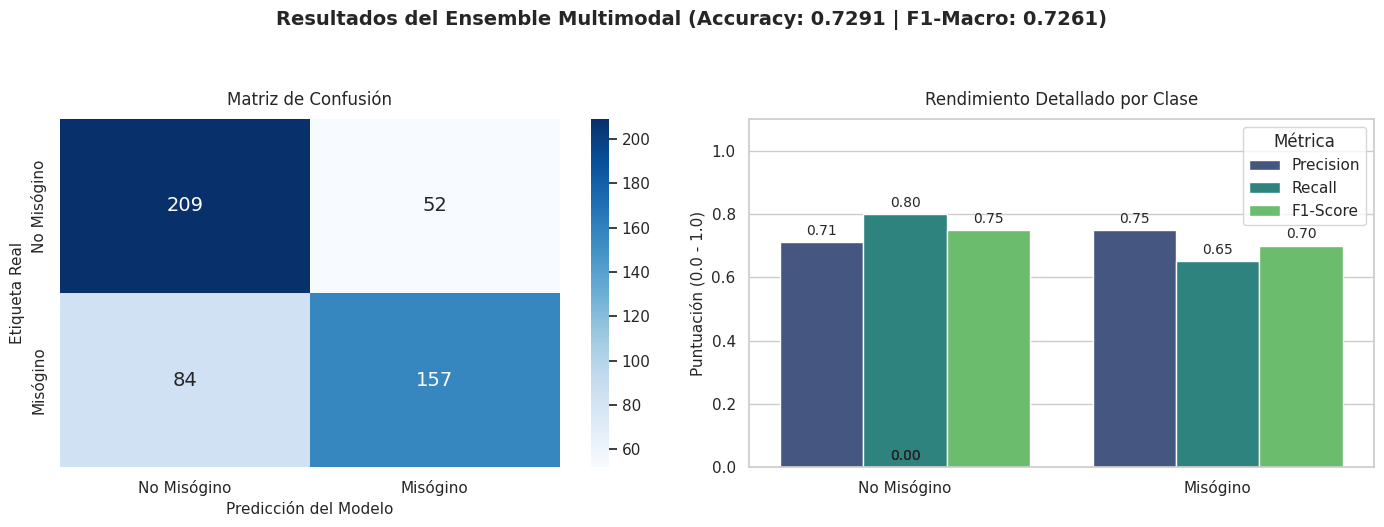
\includegraphics[width=0.9\textwidth]{Figuras/ResultadosEnsemble.png}
    \caption{Resultados del \textit{Ensemble} Multimodal contra el conjunto local de desarrollo}
    \label{fig:ResultadosEnsemble}
\end{figure}

\subsection{Análisis de Errores}
\label{subsec:AnalisisDeErrores}
Esta subsección tiene como objetivo detallar los errores cometidos por el sistema \textit{Ensemble} multimodal, buscando patrones o causas subyacentes que expliquen los fallos del modelo. No se trata únicamente de cuantificar las equivocaciones, sino de interpretarlas, comprendiendo en qué escenarios la inteligencia artificial encuentra dificultades para procesar la complejidad, el sarcasmo o la ambigüedad del lenguaje humano en las redes sociales. 

Sobre el conjunto local de desarrollo (502 instancias), el sistema generó un total de 136 predicciones erróneas. La contabilización de estas instancias en su matriz de confusión reveló un claro desbalance en el tipo de equivocación: 84 correspondieron a Falsos Negativos (el sistema no detectó el sexismo presente) y 52 a Falsos Positivos (el sistema generó una alarma falsa en un contenido inofensivo), acompañados de 209 Verdaderos Negativos y 157 Verdaderos Positivos. Esta distribución sugiere que el modelo adoptó una postura ligeramente conservadora, tendiendo a pasar por alto el sexismo cuando este se presenta de forma implícita o sutil. 

Es fundamental matizar que las explicaciones detalladas a continuación deben considerarse como interpretaciones razonables del comportamiento de la red neuronal. Al no haber implementado técnicas de Explicabilidad Algorítmica (\textit{XAI}) que muestren de forma empírica la atención de la red a características concretas, las causas atribuidas actúan como hipótesis derivadas de la observación. 

\subsubsection*{Identificación de errores comunes y ejemplos}
\label{subsubsec:IdentificacionDeErroresComunesYEjemplos}
Se estableció un protocolo de revisión cualitativa mediante el cual analizamos y codificamos manualmente una muestra de los 30 casos en los que el modelo mostró mayor ``confianza'' al equivocarse (es decir, aquellos donde la probabilidad arrojada estaba más alejada del umbral de decisión). Esto permitió agrupar los siguientes escenarios problemáticos:
\begin{itemize} 
    \item \underline{Ejemplo 1}: Violencia accidental confundida con violencia de género (Falso Positivo) 
    \begin{itemize} 
        \item \textbf{Texto}: ``\textit{cristiano ronaldo le regaló su camiseta a la guardia de seguridad que golpeó accidentalmente con un balonazo [...] la fuerza del pelotazo pues provocó que esta cayera al suelo por lo que tuvo inmediata atención...}''
        \item \textbf{Etiqueta real}: No sexista (0) | \textbf{Predicción}: Sexista (1)
        \item \textbf{Hipótesis}: Es altamente probable que el modelo asocie palabras clave de su vocabulario como ``golpeó'', ``cayera al suelo'' y ``mujer'' directamente con violencia física o machismo. Al carecer de la capacidad de abstracción para entender el contexto periodístico de un accidente deportivo, se dispara una falsa alarma.  
    \end{itemize}   
    \item \underline{Ejemplo 2}: Violencia digital contra grupos no objetivo de la tarea (Falso Positivo) 
    \begin{itemize} 
        \item \textbf{Texto}: ``\textit{el pibe inalcanzable que nunca dijo ni 'hola' en clase. se filtra su pack. compartan, compartan, muchachos, compartan...}''
        \item \textbf{Etiqueta real}: No sexista (0) | \textbf{Predicción}: Sexista (1)
        \item \textbf{Hipótesis}: El sistema detecta correctamente un patrón claro de un delito de violencia digital (difusión no consentida de imágenes íntimas mediante la palabra ``pack'' y la incitación a ``compartir''). Sin embargo, falla al razonar la directriz principal del reto: el sujeto pasivo de este escenario es un varón (el ``pibe''). Por consiguiente, aunque el texto describe un comportamiento tóxico, queda fuera de la definición estricta de discurso sexista o misógino contra la mujer que rige la construcción del \textit{dataset}, generando un falso positivo algorítmico.  
    \end{itemize} 
    \item \underline{Ejemplo 3}: \textit{Objectification} enmascarada y ruido de plataforma (Falso Negativo)
    \begin{itemize} 
        \item \textbf{Texto}: ``\textit{reply to stay smiling friends replying to yourmommaluvsthed's comment, i find chicks with jacked up teeth attractive. you must be in kentucky...}''
        \item \textbf{Etiqueta real}: Sexista (1) | \textbf{Predicción}: No sexista (0)
        \item \textbf{Hipótesis}: El mensaje contiene una clara cosificación y un uso despectivo hacia las mujeres (``\textit{chicks}''), pero el modelo no logró captar el sesgo implícito. Una posible explicación radica en que la ofensa es sutil, presentándose como una falsa preferencia estética. Además, la carga semántica está altamente diluida por los metadatos de la propia red social (``\textit{replying to... comment}''), una estructura sintáctica atípica de \textit{TikTok} que evadió los filtros de limpieza, lo que podría haber dificultado que el mecanismo de atención de la red se enfocase en la parte ofensiva.
    \end{itemize}
\end{itemize}

\subsubsection*{Errores por longitud y origen del texto}
\label{subsubsec:ErroresPorLongitudYOrigenDelTexto}
Al observar los errores en función de la estructura de las transcripciones, se registraron patrones descriptivos de interés. En primer lugar, la longitud media de los textos mal clasificados (91 palabras) resultó ser inferior a la media global del \textit{dataset} (103 palabras). Aunque sería necesario un análisis estadístico por intervalos para confirmar una correlación significativa, esta observación preliminar sugiere que los mensajes excesivamente cortos podrían privar a los modelos del contexto semántico necesario para entender la ironía o el sarcasmo, resultando en interpretaciones literales.

En segundo lugar, se identificó un desafío derivado de la diversidad en las fuentes del texto de entrada. La variable \texttt{text} proporcionada agrupa de forma indiferenciada texto proveniente de subtítulos superpuestos capturados por \textit{OCR}, transcripciones automáticas de voz (\textit{ASR}) e, incluso, metadatos y menciones a usuarios de la propia plataforma. Esta combinación produce transcripciones con nombres aleatorios y graves errores fonéticos o tipográficos. Planteamos la hipótesis de que esta densidad de ruido estructurado influye en la capacidad del modelo de aislar de manera precisa el verdadero discurso de odio del mensaje.

\subsubsection*{Reflexiones y posibles mejoras}
\label{subsubsec:ReflexionesYPosiblesMejoras}
El análisis cualitativo de estos fallos permite trazar líneas claras de trabajo a futuro. Una posible mejora radicaría en la aplicación de un preprocesamiento mucho más avanzado sobre el corpus, incorporando modelos de corrección ortográfica e identificadores de entidades nombradas para purgar nombres de usuario y menciones atípicas. 

Asimismo, se podrían generar más ejemplos de sexismo benevolente, humor sarcástico e incidentes violentos no relacionados con el género, para que el sistema aprenda a definir las fronteras o límites del sexismo. Finalmente, el uso de modelos auxiliares previamente entrenados en la detección exclusiva de ironía podría añadirse al \textit{Ensemble} como una característica de entrada adicional, ayudando a mitigar la alta tasa de Falsos Negativos detectada.

A modo de conclusión general, la optimización del sistema \textit{Ensemble} indica un buen ajuste a este complejo contenido, alcanzando un pico de \textit{Accuracy} local de 0.7291 y un \textit{F1-score} de 0.7261. Reiteramos que es fundamental interpretar este valor de 0.7261 como una métrica de calibración interna ajustada al conjunto exploratorio.  

De hecho, un análisis profundo revela sesgos predictivos importantes inherentes a esta calibración. Si observamos el rendimiento detallado por clase (apoyado en la matriz de TN=209, FP=52, FN=84 y TP=157), el modelo muestra un comportamiento notoriamente conservador: es más robusto al identificar instancias inofensivas (\textit{Recall} de 0.80 para la clase No Sexista) que al detectar agresiones reales (\textit{Recall} de 0.65 para la clase Sexista). 

Esta diferencia de 15 puntos porcentuales es la causa directa de la acumulación de Falsos Negativos. En la práctica, el ajuste del sistema priorizó no penalizar a usuarios inocentes (manteniendo bajos los Falsos Positivos), a costa de permitir que discursos de odio sutiles o enmascarados bajo ironía eludan el filtro. 

\subsection{Evaluación Final sobre el Conjunto de \textit{Test Ciego}}
\label{subsec:EvaluacionFinalTestCiego}
Tras la calibración interna del sistema explicada en las secciones anteriores, se procedió a la fase de evaluación definitiva. Con el objetivo de validar verdaderamente el modelo, se ejecutó la inferencia completa sobre el conjunto de \textit{Test} ciego oficial proporcionado por la organización del reto \textit{EXIST 2025} (compuesto por 674 vídeos sin etiquetar), el cual garantiza la separación rigurosa de autores para evitar fuga de información.

Las predicciones binarias generadas por el \textit{Ensemble} fueron enviadas a la plataforma oficial de evaluación del reto \footnote{\url{https://evall.uned.es/}}. En la \autoref{tab:ResultadosOficialesEnsemble} se presentan las métricas finales emitidas por el sistema \textit{PyEvALL}.

\begin{table}[H]
    \centering
    \begin{tabular}{lcccc}
        \toprule
        \textbf{Envío Oficial} & 
        \textbf{\begin{tabular}[c]{@{}c@{}}Ranking \\ Hipotético\end{tabular}} & 
        \textbf{ICM-Hard} & 
        \textbf{\begin{tabular}[c]{@{}c@{}}ICM-Hard \\ Norm\end{tabular}} & 
        \textbf{F1 Macro} \\
        \midrule
        \begin{tabular}[c]{@{}l@{}}\textit{Ensemble Multimodal} \\ (\textit{Late Fusion})\end{tabular} & 34 & -0.1008 & 0.4491 & 0.6311 \\
        \bottomrule
    \end{tabular}
    \caption{Resultados oficiales obtenidos en la Subtarea 3.1 de \textit{EXIST 2025} con el modelo \textit{Ensemble}}
    \label{tab:ResultadosOficialesEnsemble}
\end{table}

Al contrastar esta evaluación independiente con las métricas de las entregas unimodales iniciales del reto (detalladas previamente en la \autoref{tab:ResultadosOficialesEXIST}), se observa una mejora en el rendimiento del sistema. El \textit{Ensemble} alcanza un \textit{ICM Norm} de 0.4491, superando el 0.4355 de nuestro mejor envío oficial (\textit{BERT}) y distanciándose significativamente del 0.2874 obtenido por el modelo generativo \textit{LLaMA}.

Como es habitual en este tipo de investigaciones, se registra una caída en el rendimiento al pasar del entorno de selección local (\textit{F1}: 0.7261) al entorno ciego (\textit{F1}: 0.6311), evidenciando el \textit{overfitting} del conjunto exploratorio reutilizado y la dificultad que presentan las nuevas distribuciones de datos. Sin embargo, la evolución positiva respecto a los \textit{baselines} oficiales sugiere que la estrategia de fusión multimodal aporta una mayor robustez frente al problema. La combinación del análisis espacial de la imagen con la transcripción textual resulta de gran utilidad para contextualizar el mensaje, mitigando parte de la ambigüedad presente en las redes sociales y estableciendo una base más sólida para la moderación automática. 

\section{Perspectivismo en \textit{LeWiDi}}
\label{sec:PerspectivismoEnLewidi}
El reto \textit{EXIST 2025} introduce un desafío pionero en el campo de la detección del sexismo: la noción de que el sexismo, especialmente en sus formas más sutiles (como micromachismos y paternalismos), no siempre goza de un consenso absoluto. La percepción de si un comentario es sexista o inofensivo puede variar significativamente dependiendo de los sesgos culturales, las vivencias personales y, particularmente, el género del individuo que lo evalúa. Esta pluralidad de visiones se fundamenta teóricamente en el \textbf{Perspectivismo}, un concepto que reconoce la subjetividad en la interpretación del discurso. En el ámbito del aprendizaje automático, esta noción se materializa a través del paradigma \textbf{\textit{Learning with Disagreement} (\textit{LeWiDi})}, el cual defiende que el desacuerdo empírico entre anotadores no es un ``ruido'' estadístico que deba limpiarse, sino una señal rica en información que debe modelarse.

En las secciones anteriores, los modelos se entrenaron mediante ``Consenso Mayoritario'' (fusionando todas las opiniones en una sola etiqueta unificada). En esta última fase experimental referente a la Tarea 3.1, se buscará explorar cómo varía el rendimiento empírico de las redes neuronales cuando se filtran los datos de entrenamiento por el género del anotador o se instruye a un modelo generativo a simular un rol. 

\subsection{Segmentación demográfica en \textit{Transformers}}
\label{subsec:SegmentacionDemograficaEnTransformers}
La primera aproximación al perspectivismo consistió en entrenar modelos discriminativos independientes basados en los datos demográficos de los anotadores humanos. A partir del conjunto de entrenamiento maestro, se extrajeron de forma aislada los votos emitidos exclusivamente por los anotadores masculinos y, en paralelo, los emitidos por las anotadoras femeninas. 

Dado que un mismo vídeo podía ser evaluado por varios anotadores del mismo género (por ejemplo, dos hombres), surgieron casos de empate o ``disidencia interna'' (un hombre etiquetando como 1 y otro como 0). Para abordar este desacuerdo interno de manera metodológica y utilizando la arquitectura \texttt{RoBERTa-base}, se entrenaron 8 conjuntos de datos distintos (4 estrategias x 2 géneros): 
\begin{itemize}
    \item \textbf{Descartes (\textit{Hard Consensus})}: Se eliminaron del entrenamiento aquellos vídeos en los que los anotadores humanos del mismo género no lograron ponerse de acuerdo. 
    \item \textbf{Ante la duda, Sexismo (\textit{Pessimistic})}: En caso de empate interno humano, el video se etiquetó como sexista (1).
    \item \textbf{Ante la duda, No Sexismo (\textit{Optimistic})}: En caso de empate interno humano, prevaleció la presunción de inocencia y se etiquetó como no sexista (0).
    \item \textbf{Desenrollado (\textit{Unrolling})}: No se forzó ningún consenso. Si un vídeo presentaba empate, se introdujo dos veces en el dataset: una fila con etiqueta 1 y otra fila idéntica con etiqueta 0, obligando al modelo a asimilar la dualidad de la anotación.
\end{itemize}

Para interpretar de forma científica los resultados de esta fase, es fundamental analizar la distribución resultante tras aplicar estas estrategias. En la \autoref{tab:DistribucionPerspectivismo} se exponen los tamaños y el balance de clases de cada subconjunto de datos.

\begin{table}[H]
    \centering
    \begin{tabular}{llccc}
    \toprule
    \textbf{Estrategia} & \textbf{Género} & \textbf{Total Vídeos} & \textbf{No Sexista (0)} & \textbf{Sexista (1)} \\
    \midrule
    \multirow{2}{*}{Descartes} & Femenino & 1984 & 1035 & 949 \\
    & Masculino & 1396 & 787 & 609 \\
    \midrule
    \multirow{2}{*}{\textit{Pessimistic}} & Femenino & 2006 & 1035 & 971 \\
    & Masculino & 1612 & 787 & 825 \\
    \midrule
    \multirow{2}{*}{\textit{Optimistic}} & Femenino & 2006 & 1057 & 949 \\
    & Masculino & 1612 & 1003 & 609 \\
    \midrule
    \multirow{2}{*}{\textit{Unrolling}} & Femenino & 2644 & 1372 & 1272 \\
    & Masculino & 1948 & 1056 & 892 \\
    \bottomrule
    \end{tabular}
    \caption{Distribución de los \textit{datasets} de entrenamiento tras la segmentación por género y aplicación de estrategias de resolución de empates.}
    \label{tab:DistribucionPerspectivismo}
\end{table}

Debe reconocerse una limitación a la hora de comparar estos modelos frente al conjunto local de desarrollo (\textit{Gold Standard} unificado de 502 instancias). Como se evidencia en la tabla, existe un factor: los \textit{datasets} basados en anotaciones femeninas poseen un mayor volumen de datos que los masculinos. Por tanto, las variaciones en el rendimiento no pueden atribuirse exclusivamente a diferencias intrínsecas en la perspectiva de género, sino que podrían estar directamente influenciadas por la diferencia en la cantidad de ejemplos expuestos a la red durante el entrenamiento.

\begin{figure}[H]
    \centering
    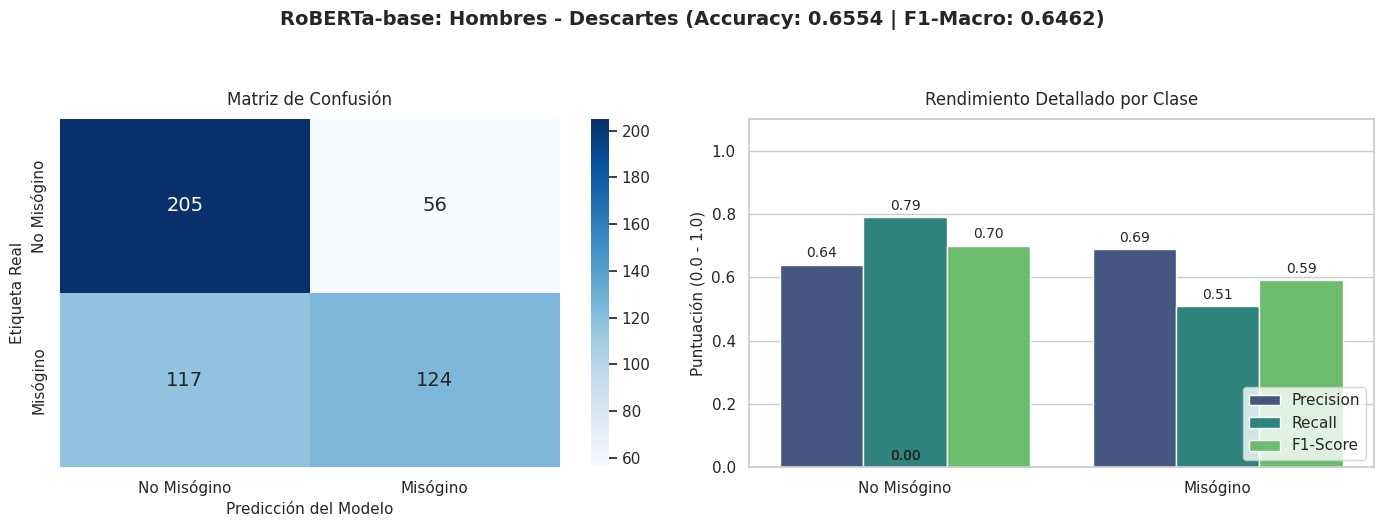
\includegraphics[width=0.9\textwidth]{Figuras/ResultadosHombreDiscard.png}
    \caption{Resultados de la estrategia \textit{Hard Consensus} en hombres}
    \label{fig:ResultadosTransformersPerspectivismoHombreDiscard}
\end{figure}
\begin{figure}[H]
    \centering
    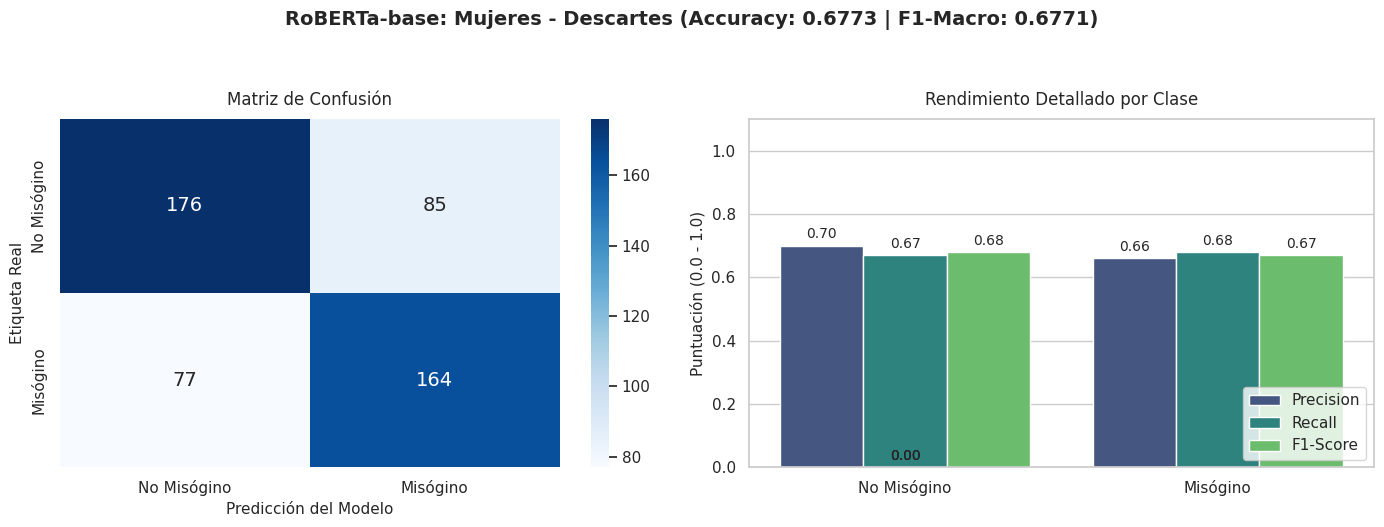
\includegraphics[width=0.9\textwidth]{Figuras/ResultadosMujerDiscard.png}
    \caption{Resultados de la estrategia \textit{Hard Consensus} en mujeres}
    \label{fig:ResultadosTransformersPerspectivismoMujerDiscard}
\end{figure}

En la \autoref{fig:ResultadosTransformersPerspectivismoHombreDiscard} y en la \autoref{fig:ResultadosTransformersPerspectivismoMujerDiscard}, se evaluó el rendimiento tras aplicar la estrategia de Descartes:
\begin{itemize}
    \item \textbf{Perspectiva Femenina}: El modelo entrenado con estos datos logra un \textit{F1-score} de 0.6771. Según se observa en su respectiva matriz de confusión, identifica 164 Verdaderos Positivos frente a los 124 del modelo masculino, alcanzando un \textit{Recall} de 0.68 para la clase sexista.
    \item \textbf{Perspectiva Masculina}: Presenta un \textit{F1-score} de 0.6462. Como evidencia su matriz, su \textit{Recall} para la clase sexista decae a 0.51, registrando 117 Falsos Negativos frente a 124 Verdaderos Positivos sobre el conjunto de validación unificado.
\end{itemize}

\begin{figure}[H]
    \centering
    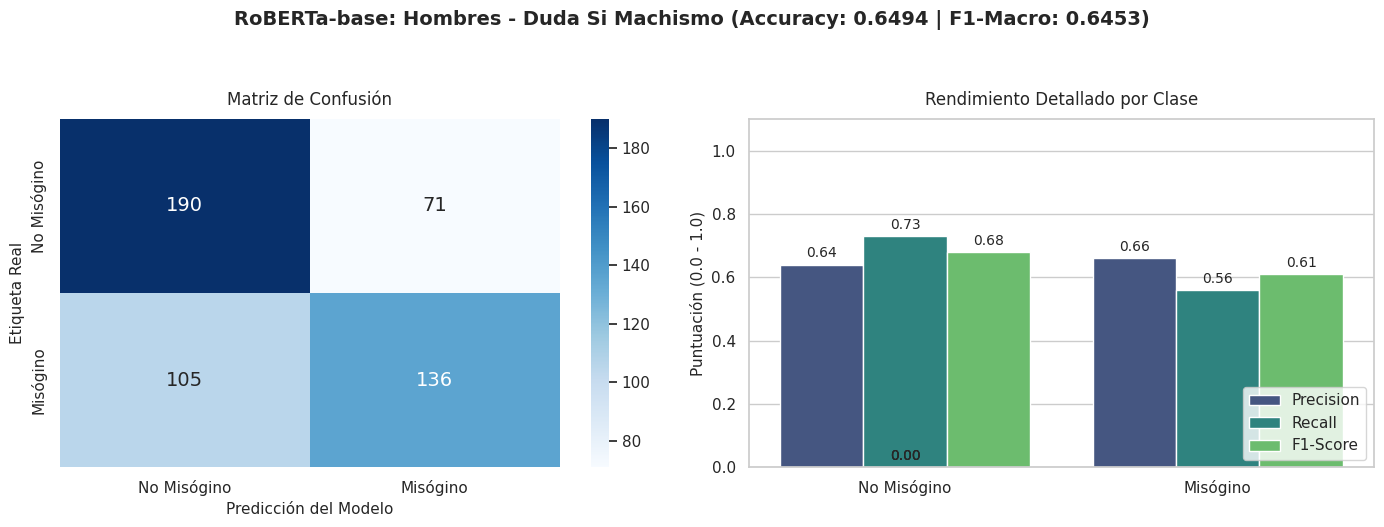
\includegraphics[width=0.9\textwidth]{Figuras/ResultadosHombrePessimistic.png}
    \caption{Resultados de la estrategia \textit{Pessimistic} en hombres}
    \label{fig:ResultadosTransformersPerspectivismoHombrePessimistic}
\end{figure}
\begin{figure}[H]
    \centering
    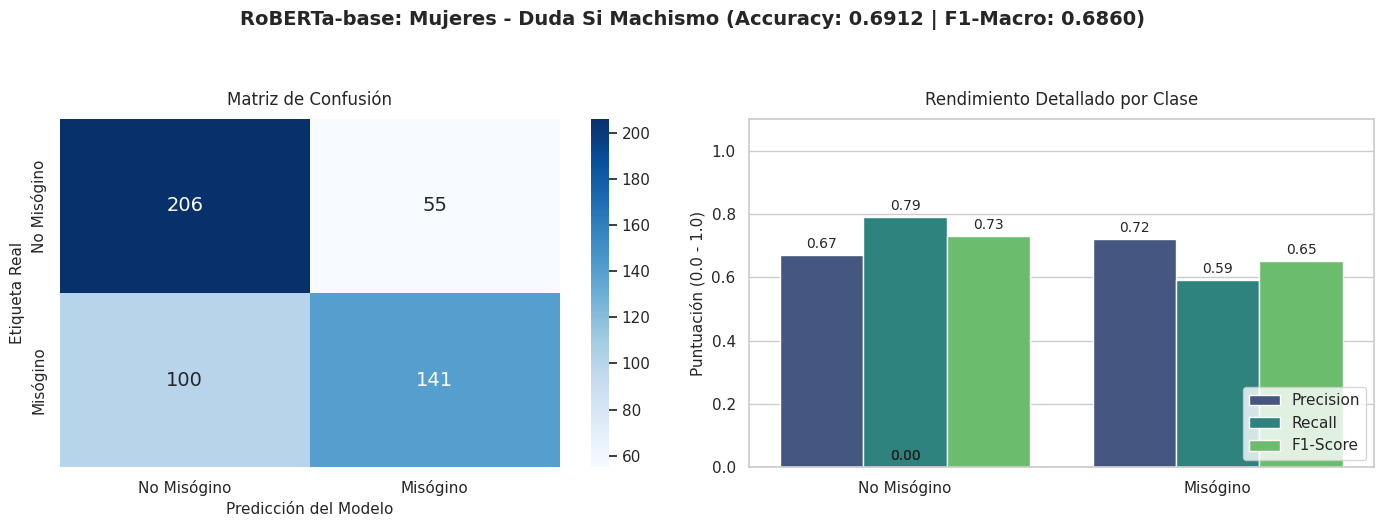
\includegraphics[width=0.9\textwidth]{Figuras/ResultadosMujerPessimistic.png}
    \caption{Resultados de la estrategia \textit{Pessimistic} en mujeres}
    \label{fig:ResultadosTransformersPerspectivismoMujerPessimistic}
\end{figure}

En la \autoref{fig:ResultadosTransformersPerspectivismoHombrePessimistic} y en la \autoref{fig:ResultadosTransformersPerspectivismoMujerPessimistic}, asumiendo la etiqueta sexista en caso de empate humano, las métricas muestran el siguiente comportamiento:
\begin{itemize}
    \item \textbf{Perspectiva Femenina}: Alcanza aquí el mejor rendimiento global registrado en esta fase (\textit{F1-score} de 0.6860). La adopción de esta postura conservadora no dispara de forma descontrolada los Falsos Positivos, conservando una \textit{Precisión} de 0.72 para la clase positiva.
    \item \textbf{Perspectiva Masculina}: El modelo disminuye su rendimiento bajo esta directriz (F1: 0.6453). Al obligarle a asumir la etiqueta sexista en los empates, el modelo incrementa los errores al clasificar instancias de la clase 0.
\end{itemize}

\begin{figure}[H]
    \centering
    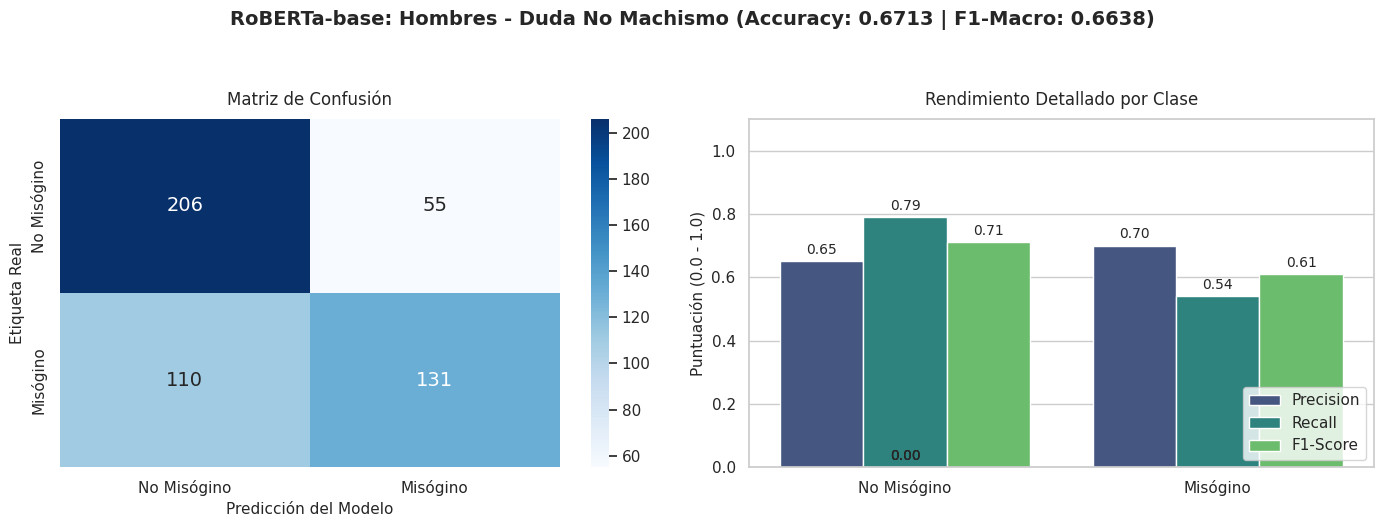
\includegraphics[width=0.9\textwidth]{Figuras/ResultadosHombreOptimistic.png}
    \caption{Resultados de la estrategia \textit{Optimistic} en hombres}
    \label{fig:ResultadosTransformersPerspectivismoHombreOptimistic}
\end{figure}
\begin{figure}[H]
    \centering
    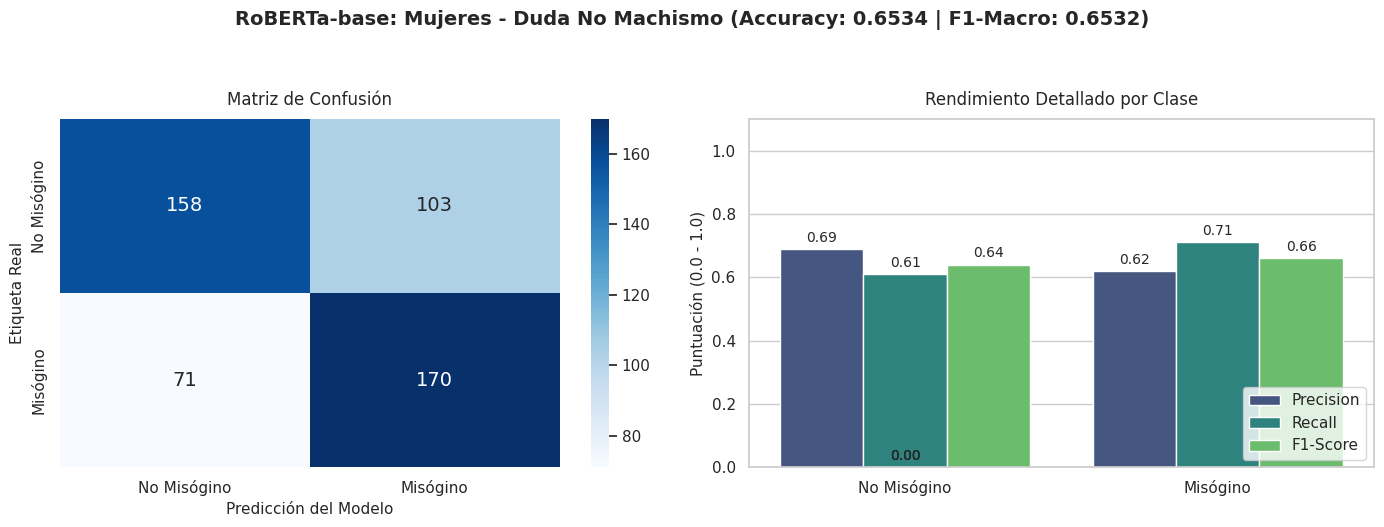
\includegraphics[width=0.9\textwidth]{Figuras/ResultadosMujerOptimistic.png}
    \caption{Resultados de la estrategia \textit{Optimistic} en mujeres}
    \label{fig:ResultadosTransformersPerspectivismoMujerOptimistic}
\end{figure}

En la \autoref{fig:ResultadosTransformersPerspectivismoHombreOptimistic} y en la \autoref{fig:ResultadosTransformersPerspectivismoMujerOptimistic}, asumiendo la etiqueta no sexista en los empates, se observa:
\begin{itemize}
    \item \textbf{Perspectiva Masculina}: El modelo presenta un \textit{Recall} de 0.54 para la clase sexista, arrojando 110 Falsos Negativos en su matriz frente a los datos del \textit{Gold Standard}.
    \item \textbf{Perspectiva Femenina}: Su \textit{Recall} para la clase sexista se sitúa en 0.71, reduciendo los Falsos Negativos a 71.
\end{itemize}

\begin{figure}[H]
    \centering
    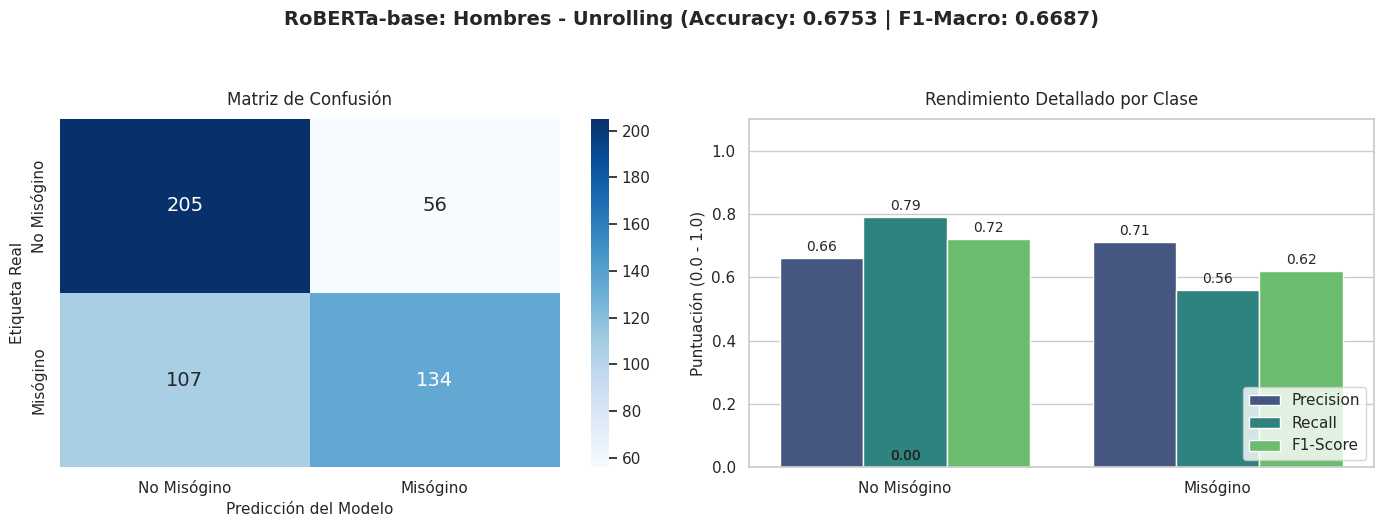
\includegraphics[width=0.9\textwidth]{Figuras/ResultadosHombreUnrolling.png}
    \caption{Resultados de la estrategia \textit{Unrolling} en hombres}
    \label{fig:ResultadosTransformersPerspectivismoHombreUnrolling}
\end{figure}
\begin{figure}[H]
    \centering
    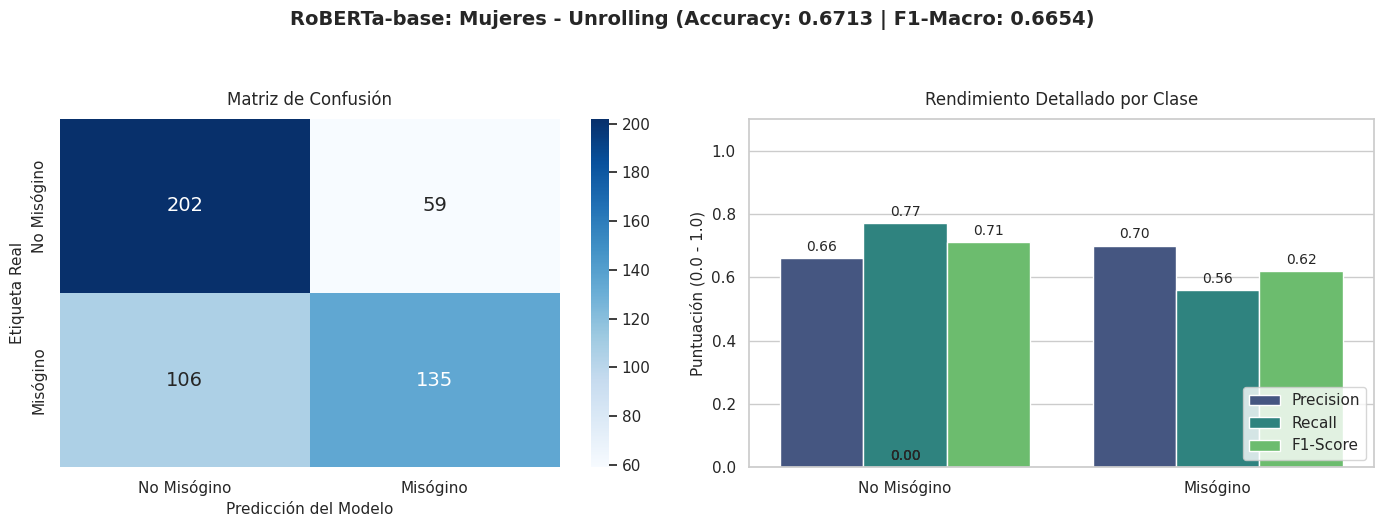
\includegraphics[width=0.9\textwidth]{Figuras/ResultadosMujerUnrolling.png}
    \caption{Resultados de la estrategia \textit{Unrolling} en mujeres}
    \label{fig:ResultadosTransformersPerspectivismoMujerUnrolling}
\end{figure}

Como podemos observar en la \autoref{fig:ResultadosTransformersPerspectivismoHombreUnrolling} y en la \autoref{fig:ResultadosTransformersPerspectivismoMujerUnrolling}, la aplicación de \textit{Unrolling} produce un ajuste evidente en ambos perfiles: 
\begin{itemize}
    \item \textbf{Convergencia de métricas}: Al duplicar los datos empatados, las diferencias de rendimiento entre el conjunto de entrenamiento de hombres (\textit{F1-score}: 0.6687) y el de mujeres (\textit{F1-score}: 0.6654) prácticamente desaparecen.
    \item \textbf{Análisis}: Ambos modelos calcan sus métricas de \textit{Recall} para la clase Sexista (0.56). Esta similitud sugiere que la estrategia de desenrollado, al exponer a la red a la dualidad de las etiquetas, homogeneiza el comportamiento predictivo, difuminando el impacto del filtrado demográfico original.
\end{itemize}

\subsection{Análisis de Sensibilidad al \textit{Prompt} en \textit{LLMs} (\textit{Persona Prompting})}
\label{subsec:InyeccionDeRolesEnLLMs}
La segunda estrategia evaluó la sensibilidad de los modelos generativos ante variaciones semánticas en la instrucción (\textit{Prompt Engineering}). Es esencial clarificar que el objetivo de este experimento no es simular de forma válida perspectivas humanas reales, sino cuantificar cómo la alteración explícita de la palabra clave asociada al género en el \textit{prompt} activa diferentes sesgos estadísticos preadquiridos por la inteligencia artificial.

Aprovechando la capacidad de los \textit{LLMs} para adaptar sus salidas, se aplicó la técnica de \textit{Persona Prompting} sobre el modelo \texttt{Mistral-7B-Instruct-v0.3} en un entorno \textit{Zero-Shot}. En lugar de pedirle una clasificación neutral, se diseñaron dos \textit{prompts} que inyectaron una instrucción de rol directamente en el contexto del modelo. El \textit{prompt} diseñado fue el siguiente:

\begin{tcolorbox}[colback=gray!10, colframe=gray!40, arc=4pt, boxrule=0.5pt]
    \texttt{[INST]} Actúa como un hombre. Eres un experto analizando redes sociales. Clasifica el siguiente texto en una de estas dos categorías: 'Sexista' o 'No Sexista'. Devuelve ÚNICAMENTE la etiqueta correspondiente, sin explicaciones adicionales. Texto: \{texto\} \texttt{[/INST]} 
    Etiqueta:
\end{tcolorbox}

De manera simétrica, para evaluar la instrucción opuesta, se sustituyeron exclusivamente las referencias de género (``Actúa como una mujer'', ``Eres una experta...'').

En las \autoref{fig:ResultadosPromptHombre} y \autoref{fig:ResultadosPromptMujer} se puede observar cómo la inyección del rol altera la distribución de las predicciones del modelo frente a los mismos 502 registros del \textit{Test} de desarrollo.

\begin{figure}[H]
    \centering
    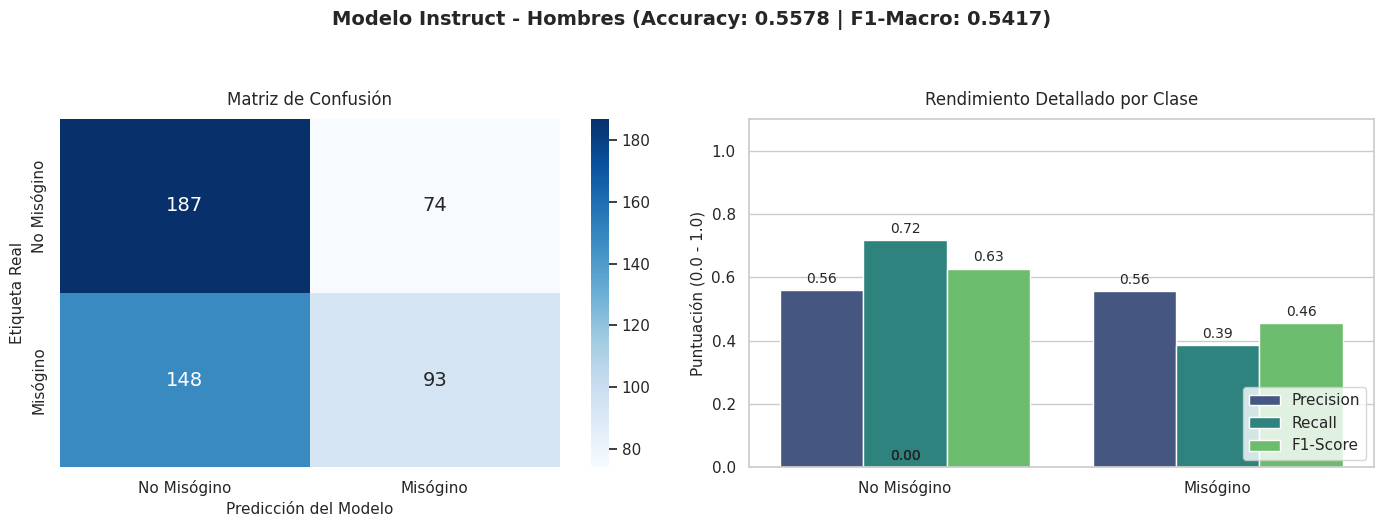
\includegraphics[width=0.9\textwidth]{Figuras/ResultadosPromptHombre.png}
    \caption{Resultados de la técnica \textit{Persona Prompting} instruyendo el rol de hombre}
    \label{fig:ResultadosPromptHombre}
\end{figure}
\begin{figure}[H]
    \centering
    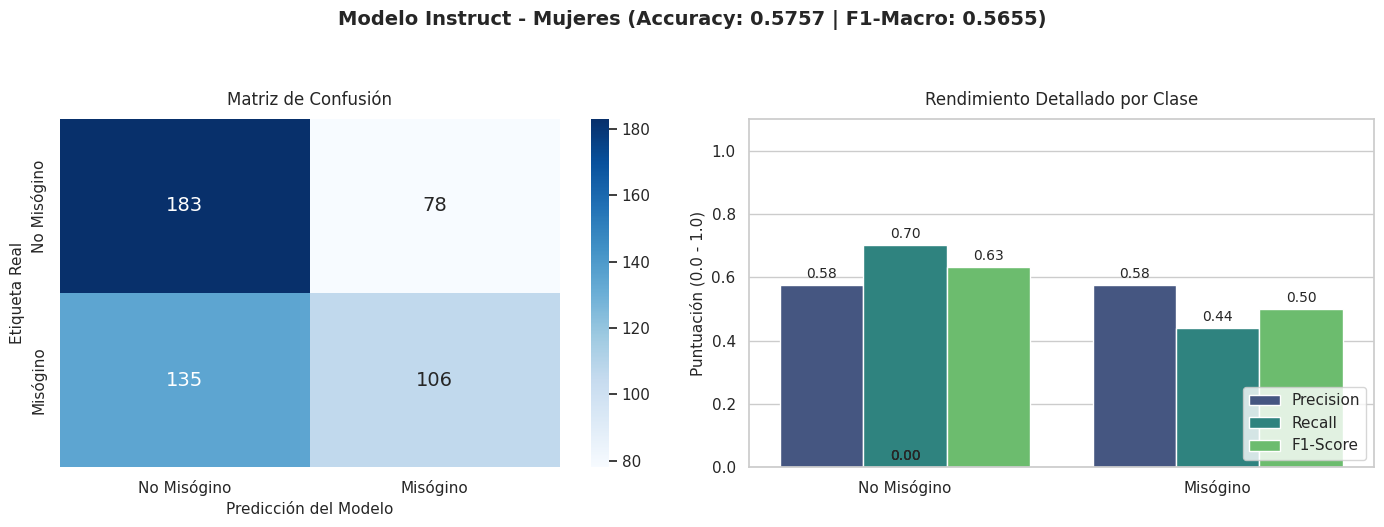
\includegraphics[width=0.9\textwidth]{Figuras/ResultadosPromptMujer.png}
    \caption{Resultados de la técnica \textit{Persona Prompting} instruyendo el rol de mujer}
    \label{fig:ResultadosPromptMujer}
\end{figure}

\subsection{Análisis de los Resultados Exploratorios}
\label{subsec:AnalisisDeLosResultadosDePerspectivismo}
Para facilitar la comparativa de los impactos demográficos detallados en las secciones anteriores, en la \autoref{tab:ResumenPerspectivismo} se aglutinan los resultados obtenidos por todas las arquitecturas y estrategias tras la segmentación por género.

\begin{table}[H]
    \centering
    \begin{tabular}{llccc}
    \toprule
    \textbf{Arquitectura} & \begin{tabular}[c]{@{}l@{}}\textbf{Estrategia de} \\ \textbf{\textit{LeWiDi}}\end{tabular} & \textbf{Rol / Género} & \textbf{\textit{Accuracy}} & \begin{tabular}[c]{@{}c@{}}\textbf{\textit{F1-score}} \\ \textbf{(Macro)}\end{tabular} \\
    \midrule
    \multirow{8}{*}{\texttt{RoBERTa-base}} 
        & \multirow{2}{*}{\begin{tabular}[c]{@{}l@{}}Descartes \\ (\textit{Hard Consensus})\end{tabular}} 
            & Femenino & 0.6773 & 0.6771 \\
        & & Masculino & 0.6554 & 0.6462 \\
    \addlinespace[0.5em]
        & \multirow{2}{*}{\begin{tabular}[c]{@{}l@{}}\textit{Pessimistic} \\ (Duda = Sexismo)\end{tabular}} 
            & Femenino & 0.6912 & 0.6860 \\
        & & Masculino & 0.6494 & 0.6453 \\
    \addlinespace[0.5em]
        & \multirow{2}{*}{\begin{tabular}[c]{@{}l@{}}\textit{Optimistic} \\ (Duda = Inocencia)\end{tabular}} 
            & Femenino & 0.6534 & 0.6532 \\
        & & Masculino & 0.6713 & 0.6638 \\
    \addlinespace[0.5em]
        & \multirow{2}{*}{\begin{tabular}[c]{@{}l@{}}Desenrollado \\ (\textit{Unrolling})\end{tabular}} 
            & Femenino & 0.6713 & 0.6654 \\
        & & Masculino & 0.6753 & 0.6687 \\
    \midrule
    \multirow{2}{*}{\texttt{Mistral-7B-Instruct}} 
        & \multirow{2}{*}{\begin{tabular}[c]{@{}l@{}}\textit{Persona} \\ \textit{Prompting}\end{tabular}} 
            & \begin{tabular}[c]{@{}l@{}}Instrucción \\ Femenina\end{tabular} & 0.5757 & 0.5655 \\
        & & \begin{tabular}[c]{@{}l@{}}Instrucción \\ Masculina\end{tabular} & 0.5578 & 0.5417 \\
    \bottomrule
    \end{tabular}
    \caption{Rendimiento comparativo de las estrategias exploratorias filtradas por género.}
    \label{tab:ResumenPerspectivismo}
\end{table}

El análisis de estos resultados permite extraer varias observaciones descriptivas sobre el comportamiento de las redes neuronales en este escenario. En primer lugar, los modelos \textit{Transformers} entrenados con los \textit{datasets} femeninos alcanzaron de forma consistente métricas más altas frente al \textit{Gold Standard} unificado (pico de \textit{F1-score} de 0.6860) que sus contrapartes masculinas (cuyo máximo se situó en 0.6687). No obstante, como se advirtió previamente, el riesgo de un sesgo por el tamaño de la muestra impide concluir con seguridad que existan características superiores en dichas anotaciones.
 
En segundo lugar, se observan diferencias ante la gestión empírica de la duda. Mientras que la variante \textit{Pessimistic} maximizó el rendimiento en el \textit{dataset} filtrado femenino, en el caso del masculino la mejor respuesta se obtuvo preservando la ambigüedad mediante \textit{Unrolling}.

Finalmente, los resultados de \textit{Persona Prompting} evidencian la adaptación de los \textit{LLMs} a los sesgos inducidos por la formulación de la instrucción. El modelo instruido con la palabra ``mujer'' logró un \textit{F1-score} de 0.5655, frente al 0.5417 arrojado bajo la instrucción ``hombre''. Al examinar sus matrices, el \textit{prompt} masculino generó una tasa mayor de Falsos Negativos (148 instancias frente a las 135 generadas por el \textit{prompt} femenino). Planteamos como hipótesis que la inyección de la palabra ``hombre'' activa estereotipos estadísticos preentrenados en la red que  derivan en una evaluación más restrictiva a la hora de tipificar el sexismo.

Es importante remarcar que el diseño metodológico de toda esta fase es de naturaleza exploratoria. Las métricas exponen el comportamiento de los modelos y las variaciones de los \textit{datasets}, y en ningún caso deben extrapolarse para formular juicios psicológicos o sociológicos sobre el comportamiento real de hombres y mujeres.

\section{Experimentación Multietiqueta (Tarea 3.3)}
\label{sec:ExperimentacionMultietiqueta}
La Tarea 3.3 del desafío \textit{EXIST 2025} plantea un problema de clasificación mucho más específico y complejo que la mera detección binaria, estructurándose como un reto jerárquico y multietiqueta. En su formulación original, el sistema debe primero discriminar si un contenido es sexista o inofensivo (primer nivel de la jerarquía) y, únicamente en caso afirmativo, categorizarlo en una o varias de cinco tipologías concretas simultáneamente (clasificación multietiqueta en el segundo nivel).

Cabe matizar explícitamente que la experimentación detallada en esta sección constituye un análisis parcial y exploratorio de las capacidades de los modelos para fines puramente académicos, por lo que no reproduce la evaluación jerárquica completa de la subtarea 3.3 oficial de \textit{EXIST 2025}. Para acotar el alcance de este Trabajo de Fin de Máster, se ha definido un análisis condicionado: se asume que el primer nivel jerárquico ya está resuelto, filtrando el conjunto de datos para evaluar a los modelos exclusivamente sobre los vídeos que ya estaban catalogados previamente como sexistas.

Asimismo, en lugar de desplegar una única arquitectura compleja con una capa de salida multietiqueta conjunta, el problema se ha abordado de forma simplificada mediante una estrategia conocida como \textit{Binary Relevance} o \textit{One-vs-Rest}. Se ha aislado cada categoría y se han entrenado clasificadores binarios independientes para cada tipología. Si bien esto simplifica la fase de optimización, conlleva una limitación estructural: las redes no son capaces de aprender las posibles correlaciones entre las distintas categorías de sexismo.

Bajo este entorno controlado, las cinco categorías evaluadas son:
\begin{itemize}
    \item \textbf{\textit{Ideological and Inequality}}: El texto desacredita el movimiento feminista, rechaza la desigualdad de género o victimiza a un hombre. 
    \item \textbf{\textit{Stereotyping and Dominance}}: Expresa ideas falsas sobre los roles de la mujer (sumisa o cuidadora) o tareas inadecuadas, afirmando la superioridad masculina. 
    \item \textbf{\textit{Objectification}}: Presenta a la mujer como un objeto, describiendo cualidades físicas obligatorias para cumplir cánones de belleza o hipersexualización.
    \item \textbf{\textit{Sexual Violence}}: Sugerencias sexuales, petición de favores o acoso explícito de naturaleza sexual (violación o agresión).
    \item \textbf{\textit{Misogyny and Non-Sexual Violence}}: Expresión de odio puro y violencia no sexual hacia las mujeres. 
\end{itemize}

Para abordar esta tarea, se replicó la metodología de experimentación unimodal utilizada en la Tarea 3.1. Se seleccionó el modelo con mejor rendimiento de cada familia arquitectónica para entrenarlo de manera independiente frente a cada una de las 5 etiquetas:
\begin{itemize}
    \item \textbf{\textit{Transformers}}: \texttt{roberta-base}.
    \item \textbf{\textit{LLM}}: \texttt{Mistral-7B-Instruct}. 
    \item \textbf{Visión Estática}: \texttt{ConvNeXt}, entrenado sobre secuencias de 4 \textit{frames}.
    \item \textbf{Visión Temporal}: \texttt{TimeSFormer}, procesando 16 \textit{frames} por inferencia.
\end{itemize}

\subsection{Preparación del Dataset Multietiqueta}
\label{subsec:PreparacionDelDatasetMultietiqueta}
A diferencia de la Tarea 3.1, la naturaleza multietiqueta del problema requiere un tratamiento especial de los datos. A partir del \textit{JSON} original, se filtraron exclusivamente aquellos vídeos catalogados previamente como sexistas (etiqueta 1 en la Tarea 3.1). Para unificar las discrepancias entre anotadores respecto al tipo de sexismo detectado, se aplicó una lógica \textit{OR}: si al menos un anotador marcaba una de las cinco etiquetas en su evaluación, el vídeo se consideraba positivo para dicha clase. 

Es necesario reconocer que esta heurística de unificación transforma la incertidumbre del \textit{Learning with Disagreement} (\textit{LeWiDi}) en etiquetas rígidas (\textit{Hard Labels}), perdiendo la distribución suave original y tendiendo a sobre-representar las categorías (sesgo hacia la sensibilidad). Por tanto, estas etiquetas actúan como un terreno de calibración experimental y no deben interpretarse como una verdad absoluta y neutral.

Dado el fuerte desbalance intrínseco en la distribución de las subcategorías, la división del conjunto original en \textit{Train} (80\%) y \textit{Test} (20\%) se ejecutó mediante la función \texttt{iterative\_train\_test\_split} de la librería \texttt{skmultilearn}. Este enfoque garantiza un particionado estratificado, asegurando que las proporciones de las clases minoritarias se mantengan estables en ambos subconjuntos. A partir de este \textit{CSV} maestro, se generaron las réplicas correspondientes para el entrenamiento de visión estática y temporal. 

\subsection{Resultados y Análisis Cruzado por Tipología}
\label{subsec:ResultadosYAnalisisCruzadoPorTipologia}
El entrenamiento aislado de los cuatro mejores modelos contra las cinco etiquetas reveló un comportamiento dependiente de la modalidad de los datos (texto frente a imagen/movimiento) y de la distribución estadística de cada clase. En la \autoref{tab:ResultadosEntrenamientosMultietiqueta} se resumen las métricas \textit{F1-Score (Macro)} y \textit{Accuracy} obtenidas sobre el conjunto de \textit{Test} de desarrollo multietiqueta. Dado el enfoque de \textit{Binary Relevance}, las métricas se reportan de forma aislada por etiqueta y no se incluyen métricas globales \textit{multilabel}.

\begin{table}[H]
    \centering
    \begin{tabular}{lllcc}
        \toprule
        \textbf{Etiqueta} & \textbf{Modelo} & \textbf{Inferencia} & \textbf{Accuracy} & \textbf{F1-score} \\
        \midrule        
        \multirow{6}{*}{Ideological-Inequality} 
            & roberta-base & - & 0.7130 & \textbf{0.7050} \\
            & mistral & - & 0.4957 & 0.4473 \\
            & \multirow{3}{*}{convnext 4 frames} 
                & max-pooling & 0.5391 & 0.5391 \\
            &   & mean-pooling  & 0.6087 & 0.5859 \\
            &   & majority vote  & 0.6000 & 0.5911 \\
            & timesformer & - & 0.5957 & 0.5908 \\
        \cmidrule{2-5}
        \multirow{6}{*}{Stereotyping-Dominance} 
            & roberta-base & - & 0.6609 & \textbf{0.5963} \\
            & mistral & - & 0.6435 & 0.4429 \\            
            & \multirow{3}{*}{convnext 4 frames} 
                & max-pooling & 0.7522 & 0.4758 \\
            &   & mean-pooling  & 0.7304 & 0.5114 \\
            &   & majority vote  & 0.7391 & 0.5271 \\
            & timesformer & - & 0.7087 & 0.5624 \\
        \cmidrule{2-5}
        \multirow{6}{*}{Objectification} 
            & roberta-base & - & 0.7435 & 0.5087 \\
            & mistral & - & 0.7478 & 0.5114 \\            
            & \multirow{3}{*}{convnext 4 frames} 
                & max-pooling & 0.6043 & 0.5098 \\
            &   & mean-pooling  & 0.6957 & 0.5082 \\
            &   & majority vote  & 0.6652 & 0.5116 \\
            & timesformer & - & 0.7304 & \textbf{0.5399} \\
        \cmidrule{2-5}
        \multirow{6}{*}{Sexual Violence} 
            & roberta-base & - & 0.8522 & \textbf{0.4601} \\
            & mistral & - & 0.8522 & \textbf{0.4601} \\            
            & \multirow{3}{*}{convnext 4 frames} 
                & max-pooling & 0.8522 & \textbf{0.4601} \\
            &   & mean-pooling  & 0.8522 & \textbf{0.4601} \\
            &   & majority vote  & 0.8522 & \textbf{0.4601} \\
            & timesformer & - & 0.8522 & \textbf{0.4601} \\
        \cmidrule{2-5}
        \multirow{6}{*}{\begin{tabular}[c]{@{}l@{}}Misogyny and \\ Non-Sexual Violence\end{tabular}}            
            & roberta-base & - & 0.8217 & 0.4511 \\
            & mistral & - & 0.8043 & \textbf{0.4861} \\            
            & \multirow{3}{*}{convnext 4 frames} 
                & max-pooling & 0.8217 & 0.4511 \\
            &   & mean-pooling  & 0.8217 & 0.4511 \\
            &   & majority vote  & 0.8217 & 0.4511 \\
            & timesformer & - & 0.7913 & 0.4615 \\
        \bottomrule
    \end{tabular}
    \caption{Resultados de \textit{Accuracy} y \textit{F1-score} de cada una de las etiquetas}
    \label{tab:ResultadosEntrenamientosMultietiqueta}
\end{table}

El análisis comparativo de las métricas de rendimiento (\textit{F1-score Macro} y \textit{Accuracy}) por etiquetas arrojan tres observaciones fundamentales que sugieren cómo se comportan las redes neuronales frente al tipo de sexismo:
\begin{enumerate}
    \item \textbf{El dominio del Texto en la Ideología y el Estereotipo}: Para la etiqueta \textit{Ideological and Inequality}, el modelo puramente textual \texttt{RoBERTa-base} dominó la clasificación con un F1 de \textbf{0.7050}, muy superior al resto de modelos, incluyendo a \textit{Mistral} que obtuvo un pobre 0.4473. El contenido ideológico y político en plataformas como \textit{TikTok} recae casi exclusivamente en el discurso hablado o escrito, haciendo que las modalidades visuales (\texttt{ConvNeXt}: 0.5911, \texttt{TimeSFormer}: 0.5908) queden relegadas a un papel secundario. En la categoría \textit{Stereotyping and Dominance}, \texttt{RoBERTa} volvió a liderar (F1: 0.5963), seguido de cerca por la visión temporal (0.5624), sugiriendo que los estereotipos sí poseen una carga visual de acciones o roles que el modelo de vídeo logra captar en mejor medida que el de imagen estática.
    \item \textbf{Indicios sobre el movimiento en la Cosificación}: En la etiqueta \textit{Objectification}, los modelos de texto (\texttt{RoBERTa}: 0.5087) y de imagen estática (\texttt{ConvNeXt}: 0.5116) mostraron dificultades. Sin embargo, la arquitectura de visión temporal \texttt{TimeSFormer} logró despuntar ligeramente (F1: \textbf{0.5399}). A falta de pruebas de evaluaciones en un entorno de test ciego, este resultado sirve como un indicio exploratorio de que la cosificación en formato vídeo podría captarse con mayor eficacia modelando el movimiento (poses, movimientos de cámara o acciones sugerentes en el tiempo) que analizando un fotograma congelado.
    \item \textbf{Colapso predictivo ante el desbalanceo de clases raras}: Para las categorías extremadamente minoritarias en el \textit{dataset} (\textit{Sexual Violence} y \textit{Misogyny and Non-Sexual Violence}), los cuatro modelos sin excepción sufrieron un colapso. El valor de \textit{F1-score Macro} de \textbf{0.4601} (con un \textit{Accuracy} de 0.8522) observado en \textit{Sexual Violence} ilustra el \textit{baseline} mayoritario: debido a la extrema escasez de ejemplos positivos de violencia sexual, las redes neuronales no logran extraer patrones y optan por predecir sistemáticamente la clase negativa (0) en todas las instancias. El 0.4601 no representa un aprendizaje deficiente, sino el valor matemático resultante de obtener un \textit{Recall} perfecto en la clase mayoritaria y un cero absoluto en la minoritaria. Ninguna modalidad pudo sobreponerse a esta barrera estadística sin la aplicación previa de técnicas agresivas de \textit{Oversampling} o ajustes en la ponderación de la función de pérdida.
\end{enumerate}

\section{Resumen Global de Resultados}
\label{sec:ResumenGlobalDeResultados}

A lo largo de este capítulo, se ha desplegado una extensa batería de experimentos que abarca múltiples modalidades (texto, imagen y vídeo) y enfoques arquitectónicos (modelos discriminativos y generativos). Dada la gran cantidad de combinaciones de hiperparámetros, técnicas de \textit{Data Augmentation} y lógicas de consolidación evaluadas, resulta importante destacar los hitos más relevantes de la investigación antes de extraer las conclusiones finales.

En la \autoref{tab:ResumenGlobalMejoresModelos} se consolida exclusivamente el modelo con mejor rendimiento de cada fase experimental para la clasificación binaria de sexismo (Tarea 3.1). Esta visión panorámica permite apreciar de un vistazo la evolución de las métricas desde los \textit{baselines} iniciales hasta llegar a la solución multimodal definitiva.

\begin{table}[H]
    \centering
    \begin{tabular}{llccc}
        \toprule
        \textbf{Modalidad} & \begin{tabular}[c]{@{}l@{}}\textbf{Mejor} \\ \textbf{Arquitectura}\end{tabular} & \begin{tabular}[c]{@{}c@{}}\textbf{Técnica} \\ \textbf{Destacada}\end{tabular} & \textbf{Accuracy} & \textbf{F1-score} \\
        \midrule
        \begin{tabular}[c]{@{}l@{}}Texto \\ (\textit{Baseline})\end{tabular} & \begin{tabular}[c]{@{}l@{}}\texttt{bert-base-} \\ \texttt{multilingual-cased}\end{tabular} & \textit{Fine-Tuning} & 0.6275 & 0.6215 \\
        \begin{tabular}[c]{@{}l@{}}Texto \\ (Discrim.)\end{tabular} & \texttt{roberta-base} & \textit{Fine-Tuning} & 0.6972 & 0.6934 \\
        \begin{tabular}[c]{@{}l@{}}Texto \\ (Generativo)\end{tabular} & \texttt{Mistral-7B-Instruct} & \begin{tabular}[c]{@{}c@{}}\textit{PEFT} \\ \textit{(QLoRA)}\end{tabular} & 0.7171 & 0.7141 \\
        \midrule
        \begin{tabular}[c]{@{}l@{}}Visión \\ Estática\end{tabular} & \texttt{ConvNeXt} & \begin{tabular}[c]{@{}c@{}}4 \textit{frames} \\ (\textit{Mean-Pool})\end{tabular} & 0.6275 & 0.6245 \\
        \begin{tabular}[c]{@{}l@{}}Visión \\ Temporal\end{tabular} & \texttt{TimeSformer} & \begin{tabular}[c]{@{}c@{}}10\% \textit{Augmentation} \\ (Clase 1)\end{tabular} & 0.5956 & 0.5956 \\
        \midrule
        \begin{tabular}[c]{@{}l@{}}\textbf{Fusión} \\ \textbf{(Desarrollo)}\end{tabular} & \textbf{\textit{Ensemble} (Local)} & \begin{tabular}[c]{@{}c@{}}\textbf{\textit{Late Fusion}} \\ \textbf{(0.35/0.55/0.10)}\end{tabular} & \textbf{0.7291} & \textbf{0.7261} \\
        \begin{tabular}[c]{@{}l@{}}\textbf{Fusión} \\ \textbf{(\textit{Test} Ciego)}\end{tabular} & \textbf{\textit{Ensemble} (Oficial)} & \begin{tabular}[c]{@{}c@{}}\textbf{Evaluación} \\ \textbf{PyEvALL}\end{tabular} & \textbf{0.6418} & \textbf{0.6311} \\
        \bottomrule
    \end{tabular}
    \caption{Resumen de los mejores modelos obtenidos por modalidad para la Tarea 3.1.}
    \label{tab:ResumenGlobalMejoresModelos}
\end{table}

Como se observa empíricamente en la tabla, dentro del entorno de desarrollo local ninguna modalidad aislada fue capaz de superar al \texttt{Mistral-7B-Instruct} en la métrica \textit{F1-score}. La mejora más significativa a nivel interno se produjo al fusionar los grandes modelos de lenguaje con la extracción de características espaciales de la visión estática y temporal, sugiriendo el potencial del enfoque multimodal para el análisis del sexismo en redes sociales modernas. Si bien la evaluación independiente sobre el conjunto ciego oficial ajusta el rendimiento real del sistema a un \textit{F1-score} de 0.6311 (reflejando el sobreajuste previo al conjunto local de validación), la arquitectura unificada logra una mejora evidente frente a los envíos unimodales originales del reto.

Adicionalmente, los experimentos complementarios de la Tarea 3.3 sugirieron que la detección de tipologías específicas requiere enfoques especializados (por ejemplo, el movimiento temporal para captar la cosificación, o el texto puro para el sesgo ideológico), mientras que la experimentación exploratoria con \textit{LeWiDi} sugirió que las diferencias demográficas en la anotación podrían influir en el comportamiento del modelo, si bien este hallazgo debe interpretarse con suma cautela debido a los factores presentes en las distribuciones de los datos.
\chapter{Conclusiones y Trabajo Futuro}
\label{cap:Conclusiones}

Este capítulo ofrece una síntesis de la investigación realizada, valorando el grado de cumplimiento de los objetivos iniciales y destacando los hallazgos más relevantes obtenidos tras la extensa variedad de experimentos. Asimismo, se exponen las limitaciones encontradas, se proponen líneas de investigación futuras para dar continuidad al proyecto, y se detalla y justifica el esfuerzo temporal y computacional invertido en su desarrollo.

\section{Conclusiones}
\subsection*{Consecución de Objetivos}
La evaluación de los objetivos planteados al inicio de esta memoria muestra un grado de cumplimiento muy satisfactorio en términos generales, si bien es necesario realizar una valoración individualizada para señalar aquellos que se han alcanzado de forma parcial:
\begin{itemize}
    \item \textbf{Estudiar el estado del arte:} Cumplido. Se ha fundamentado la investigación en la literatura reciente sobre \textit{Deep Learning}, PLN y Visión Artificial aplicados a la detección de contenido de odio.
    \item \textbf{Preprocesar y adecuar el conjunto de datos:} Cumplido. Se desarrolló un \textit{pipeline} robusto de limpieza textual mediante \textit{regex} y extracción temporal de \textit{frames} mediante \textit{OpenCV}, además de implementar lógicas matemáticas para el manejo de etiquetas bajo el paradigma \textit{LeWiDi}.
    \item \textbf{Implementar y ajustar (\textit{fine-tuning}) modelos:} Cumplido. Se entrenaron y compararon con éxito arquitecturas discriminativas (\textit{RoBERTa}), generativas (\textit{Mistral}), de visión estática (\textit{ConvNeXt}) y de visión temporal (\textit{TimeSFormer}).
    \item \textbf{Proponer y desarrollar estrategias de fusión:} Cumplido. Se diseñó, optimizó y evaluó un sistema \textit{Ensemble} basado en \textit{Late Fusion} mediante la suma ponderada de probabilidades.
    \item \textbf{Participar en la tarea 3.1 de \textit{EXIST 2025}:} Cumplido. Se enviaron las predicciones oficiales utilizando \textit{BERT} y \textit{Llama} (\textit{zero-shot}), estableciendo el \textit{baseline} del proyecto.
    \item \textbf{Desarrollar marco de evaluación local (Tarea 3.1 y 3.3):} \textbf{Alcanzado parcialmente}. Si bien se generó un entorno de evaluación riguroso, el marco local de la Tarea 3.1 presentó un fuerte sesgo (\textit{overfitting}) al reutilizar el \textit{holdout} para la selección de hiperparámetros y la ponderación. Asimismo, la Tarea 3.3 no se abordó como un sistema multietiqueta jerárquico completo, sino que se condicionó a un análisis exploratorio simplificado (\textit{One-vs-Rest}) que sufrió un colapso predictivo ante el desbalanceo extremo de las clases minoritarias.
    \item \textbf{Explorar el impacto del perspectivismo:} Cumplido. Se demostró la sensibilidad algorítmica a la perspectiva de género mediante la segmentación demográfica de los anotadores y técnicas de \textit{Persona Prompting}.
\end{itemize}

\subsection*{Resumen de los Hallazgos}
Los resultados de la experimentación sugieren fuertemente que el sexismo en plataformas digitales es un fenómeno multimodal. Ningún modelo unimodal logró igualar el rendimiento del sistema unificado mediante \textit{Late Fusion} en el entorno de validación local (donde alcanzó un \textit{F1-score} de 0.7261). Al evaluar su capacidad predictiva frente al conjunto ciego oficial de la competición, el \textit{Ensemble} obtuvo un \textit{F1-score} de 0.6311. Esta caída de rendimiento evidencia la existencia de un sobreajuste (\textit{overfitting}) previo durante la fase de selección, pero, aun así, la arquitectura unificada logró una mejora objetiva frente a los enfoques individuales. El análisis exploratorio detallado indicó que el texto resulta especialmente útil para detectar cargas ideológicas, mientras que la información visual y temporal parece aportar un contexto valioso para abordar fenómenos complejos como la cosificación.

Además, los experimentos de perspectivismo han mostrado observaciones empíricas de gran valor para el diseño de IAs: la anotación del discurso de odio realizada desde una perspectiva femenina resultó en modelos con métricas de recuperación (\textit{Recall}) más sólidas. Por su parte, la simulación de roles en Grandes Modelos de Lenguaje demostró que inyectar el rol ``masculino'' en el \textit{prompt} dispara la tasa de falsos negativos. Si bien estos hallazgos están condicionados por el tamaño de los \textit{datasets} y los sesgos estadísticos preentrenados en los \textit{LLMs}, sugieren que la identidad demográfica (ya sea real o simulada) altera la evaluación algorítmica del discurso de odio.

\subsection*{Implicaciones}
Los resultados obtenidos respaldan el potencial de combinar \textit{LLMs} ajustados mediante \textit{PEFT} (\textit{QLoRA}) con \textit{Vision Transformers}. Se observa empíricamente que, para moderar plataformas modernas de vídeos cortos, el análisis de texto aislado puede resultar insuficiente, recomendándose su hibridación con la semántica del movimiento y la disposición espacial para comprender la verdadera intencionalidad del contenido.

\subsection*{Limitaciones}
La principal limitación técnica encontrada ha sido el desbalanceo extremo en las clases minoritarias del \textit{dataset} multietiqueta (especialmente en \textit{Sexual Violence} y \textit{Misogyny and Non-Sexual Violence}). Esta carencia de ejemplos positivos provocó un colapso predictivo en todas las familias de modelos, que optaron por predecir matemáticamente la clase mayoritaria. Por otro lado, hemos tenido la limitación derivada de haber reutilizado el mismo conjunto local de desarrollo para la selección de hiperparámetros y pesos del \textit{Ensemble}, lo que generó un sesgo al alza en las métricas internas reportadas. Finalmente, la extracción del texto incrustado en el vídeo introdujo ruido y ``basura algorítmica'' (como \textit{tags} y menciones) que dificultó la comprensión semántica de las redes.

\subsection*{Contribuciones}
Este trabajo aporta una metodología documentada de manera exhaustiva para el tratamiento multimodal de datos en español e inglés. Se ha analizado el comportamiento comparativo de modelos discriminativos y generativos, se han evaluado distintas lógicas estadísticas de agregación de fotogramas (\textit{Mean-Pooling, Majority-Vote}), y se ha explorado el impacto de los sesgos demográficos (\textit{LeWiDi}) en el entrenamiento de la inteligencia artificial.

\subsection*{Consideraciones Éticas}
El uso de modelos de inteligencia artificial para la moderación de contenido humano conlleva profundas implicaciones éticas. Como ha ilustrado el análisis de errores y de perspectivismo de este documento, los modelos tienden a heredar e incluso amplificar los sesgos de sus datos de entrenamiento. Las decisiones de censura o bloqueo automatizadas en redes sociales no deben ser tomadas como verdades absolutas, sino que deben contextualizarse y contar con supervisión humana para evitar la discriminación y el silenciamiento sistémico. 

\section{Trabajo Futuro}
\subsection*{Mejoras Metodológicas y Preprocesamiento}
A corto plazo, una línea de trabajo esencial consiste en implementar filtros de limpieza de texto mucho más robustos para mitigar el ruido introducido por el \textit{OCR} y las transcripciones de audio automáticas, traduciendo los metadatos visuales a un formato puramente semántico. Asimismo, resultaría crítico aplicar técnicas de \textit{Oversampling} avanzado o penalización de pesos funcionales (\textit{Class Weights}) para solventar el colapso predictivo de los modelos ante el desbalanceo de las categorías más graves.

\subsection*{Extensiones del Estudio Multimodal}
Aunque este trabajo ha fusionado texto, imagen estática y secuencias temporales de vídeo, el sonido aporta información vital no verbal (tono de voz, sarcasmo acústico, risas). Una extensión natural del sistema consistirá en integrar modelos especializados en características acústicas, como \textit{Wav2Vec} o \textit{Audio Spectogram Transformers}, añadiendo una nueva dimensión a la ecuación del \textit{Ensemble}. Además, sería interesante investigar técnicas de \textit{Early Fusion} o arquitecturas de atención cruzada (\textit{Cross-Attention}) que permitan a los modelos interconectar y evaluar texto e imagen de forma simultánea, y no en etapas separadas.


\subsection*{Aplicaciones Prácticas}
A nivel aplicado, la arquitectura híbrida documentada podría sentar las bases para una herramienta de \textit{software} capaz de asistir a los equipos de \textit{Trust \& Safety} de plataformas digitales. Esta herramienta no buscaría censurar autónomamente, sino priorizar y marcar de forma automática aquellos contenidos que, por su combinación de factores textuales y visuales, presenten una alta probabilidad de albergar discursos de odio, optimizando así el tiempo de revisión humana.

\section{Planificación Temporal del Trabajo Realizado}
En este apartado se detalla el tiempo y los recursos empleados en la investigación y redacción del presente Trabajo de Fin de Máster. Dada la magnitud de la experimentación requerida, el mayor esfuerzo no recayó en las entregas iniciales de la competición, sino en el análisis avanzado, entrenamiento y depuración de modelos a posteriori. Las horas globales estimadas se resumen en la \autoref{tab:PlanificationTemporal}.

\begin{table}[H]
    \centering
    \begin{tabularx}{\textwidth}{Xr}
        \toprule
        \textbf{Tarea} & \textbf{Horas Estimadas} \\
        \midrule
        \textbf{Revisión del Estado del Arte e Investigación Teórica:} & \textbf{50} \\
        \quad - Análisis del discurso de odio, \textit{Transformers}, y \textit{LLMs}. & \\
        \quad - Estudio del Perspectivismo (\textit{LeWiDi}) y métricas de evaluación. & \\
        \addlinespace[0.2em]
        \textbf{Familiarización con el Entorno y Tecnologías:} & \textbf{50} \\
        \quad - Despliegue en \textit{Google Colab}, librerías (\textit{PyTorch}, \textit{Hugging Face}). & \\
        \quad - Lógicas de extracción multimedia (\textit{OpenCV}, \textit{Decord}). & \\
        \addlinespace[0.2em]
        \textbf{Tratamiento de Datos y Entregas Preliminares (EXIST 2025):} & \textbf{70} \\
        \quad - Limpieza de \textit{datasets}, gestión de nulos y estructuración de \textit{frames}. & \\
        \quad - \textit{Splits} estratificados para la tarea binaria y multietiqueta. & \\
        \addlinespace[0.2em]
        \textbf{Experimentación Avanzada \textit{a posteriori} y Desarrollo:} & \textbf{140} \\
        \quad - Ejecución y entrenamiento intensivo en GPUs (entorno L4 de Colab). & \\
        \quad - \textit{Debugging}, resolución de errores de memoria (OOM), HPO. & \\
        \quad - Algoritmos de \textit{Late Fusion} y \textit{Persona Prompting} en \textit{Mistral}. & \\
        \addlinespace[0.2em]
        \textbf{Elaboración de la Memoria y Formato:} & \textbf{70} \\
        \quad - Análisis cruzado de resultados, extracción de gráficas y conclusiones. & \\
        \quad - Redacción intensiva, maquetación en \LaTeX{} y revisión final. & \\
        \midrule
        \textbf{Total} & \textbf{380} \\
        \bottomrule
    \end{tabularx}
    \caption{Estimación de la planificación temporal del trabajo realizado.}
    \label{tab:PlanificationTemporal}
\end{table}

Como se refleja en la tabla, el proyecto ha requerido una inversión aproximada de 380 horas. Cabe destacar el elevado coste computacional de la fase de Experimentación Avanzada. Durante esta etapa, se consumieron más de 300 unidades de cómputo en la plataforma \textit{Google Colab} utilizando hardware de alto rendimiento (\textit{GPUs NVIDIA L4}) para poder procesar los grandes volúmenes de datos de imágenes y vídeo, y realizar el \textit{Fine-Tuning} de arquitecturas pesadas como \textit{ConvNeXt}, \textit{TimeSFormer} y el modelo de lenguaje \textit{Mistral-7B}. Este volumen de experimentación es el que ha permitido estructurar y fundamentar los hallazgos descritos a lo largo de este documento. 

%%%%%%%%%%%%%%%%%%%%% BIBLIOGRAFÍA %%%%%%%%%%%%%%%%%%%%%%
\printbibliography[heading=bibintoc,title={Referencias}]

%%%%%%%%%%%%%%%%%%%%% ANEXOS %%%%%%%%%%%%%%%%%%%%%%
\appendix
\chapter{Anexos}
\section{Aplicación Web para la Visualización y Prueba del Modelo}
\label{ap:AplicacionWeb}
Como culminación del presente Trabajo de Fin de Máster, se ha desarrollado y desplegado una aplicación web interactiva que ejecuta el sistema multimodal completo (\textit{Ensemble} mediante \textit{Late Fusion}). Esta herramienta permite clasificar nuevas instancias de vídeo en tiempo real. 

Para superar las limitaciones de memoria VRAM (15 GB) de los entornos gratuitos y evitar el colapso del sistema, se ha diseñado una arquitectura inteligente de carga secuencial y liberación dinámica de memoria. Esto permite ejecutar iterativamente modelos masivos que, en un despliegue estático tradicional, requerirían infraestructura de alto coste.  

\section*{Arquitectura y Tecnologías Utilizadas}
Para hacer viable el despliegue del sistema \textit{Ensemble} completo (combinando \textit{Mistral}, \textit{ConvNeXt} y \textit{TimeSFormer}), la aplicación utiliza una arquitectura puente que separa el \textit{backend} de cómputo del \textit{frontend} de visualización:
\begin{itemize}
    \item \textbf{Backend y Cómputo (\textit{Google Colab})}: El núcleo de procesamiento se ejecuta en un entorno de \textit{Google Colab} equipado con una \textit{GPU NVIDIA T4}, montando \textit{Google Drive} para la carga local de los pesos de los modelos. Aquí se ejecuta la lógica pesada y la cuantización de \textit{Mistral-7B} en 4-bits mediante \textit{QLoRA}.
    \item \textbf{Túnel de Conexión (\textit{Gradio})}: Mediante la librería \textit{Gradio}, el entorno de Colab genera un túnel inverso temporal (URL pública \texttt{.gradio.live}) que expone la interfaz interactiva hacia el exterior.
    \item \textbf{Frontend Estático (\textit{Hugging Face Spaces})}: Para dotar al proyecto de una URL institucional y permanente, se ha habilitado un \textit{Space} en \textit{Hugging Face}. Dicho espacio funciona como un contenedor estático (mediante un archivo \texttt{index.html}) que embebe la interfaz generada por Colab. Por tanto, el cómputo masivo no recae sobre los limitados servidores de Hugging Face, sino sobre la GPU de Google.
\end{itemize}

Esta arquitectura implica que la disponibilidad de la aplicación está sujeta a que el cuaderno de ejecución en \textit{Google Colab} se encuentre activo.

\section*{Acceso a la Aplicación y Código Fuente}
La herramienta se encuentra vinculada para su visualización desde cualquier navegador web estándar en la siguiente URL:

\begin{center}
\textbf{\url{https://huggingface.co/spaces/visumania2/DeepSexist-App}}
\end{center}

Asimismo, con el fin de garantizar la transparencia y reproducibilidad de esta investigación, el código fuente completo del proyecto está alojado en un repositorio público. Este repositorio contiene los cuadernos de entrenamiento originales (incluyendo el historial de versiones), los \textit{scripts} de gestión del \textit{dataset} y los cuadernos de despliegue de esta misma aplicación (omitiendo los datos audiovisuales restringidos por la competición):
\begin{center}
\textbf{\url{https://github.com/visumania/DeepSexist}}
\end{center}

\section*{Manual de Usuario}
El uso de la aplicación consta del siguiente flujo simplificado:

\begin{enumerate}
    \item Acceder a la URL habilitada.
    \item Cargar un archivo de vídeo (\texttt{.mp4}, \texttt{.avi}) en el componente principal de la pantalla. 
    \item Pulsar el botón ``Ejecutar Pipeline Multimodal''.
    \item El sistema procesará de forma automatizada las vías requeridas: transcripción de audio a texto, \textit{mean-pooling} de 4 fotogramas visuales y análisis de la matriz del movimiento. 
    \item Tras el procesado, se visualizarán las probabilidades de sexismo independientes de cada modelo y el resultado final calculado por la suma ponderada del \textit{Ensemble} (35\% texto, 55\% imagen y 10\% vídeo).
\end{enumerate}

\section*{Ejemplo de Uso}
A continuación, se detalla un caso de uso práctico procesado por el \textit{Ensemble}:
\begin{itemize}
    \item \textbf{Vídeo introducido}: Clip de 15 segundos con un discurso basado en roles tradicionales. 
    \item \textbf{Transcripción automática (\textit{Whisper})}: ``\textit{El lugar de las mujeres está en casa, no en una oficina dirigiendo empresas}''. 
    \item \textbf{Modelo Texto (\textit{Mistral}-35\%)}: Probabilidad de Sexismo: 98.20\%.
    \item \textbf{Modelo Imagen (\textit{ConvNeXt}-55\%)}: Probabilidad de Sexismo: 62.40\%.
    \item \textbf{Modelo Vídeo (\textit{TimeSFormer}-10\%)}: Probabilidad de Sexismo: 71.00\%.
    \item \textbf{Resultado Final (\textit{Ensemble})}: Probabilidad del \textit{Ensemble}:75.79\%. Resultado final: \textbf{SEXISTA}.
\end{itemize}

\section*{Capturas de Pantalla}

A continuación, en la \autoref{fig:CapturaGradio} se muestra el aspecto visual de la aplicación web en funcionamiento:

\begin{figure}[H]
    \centering
    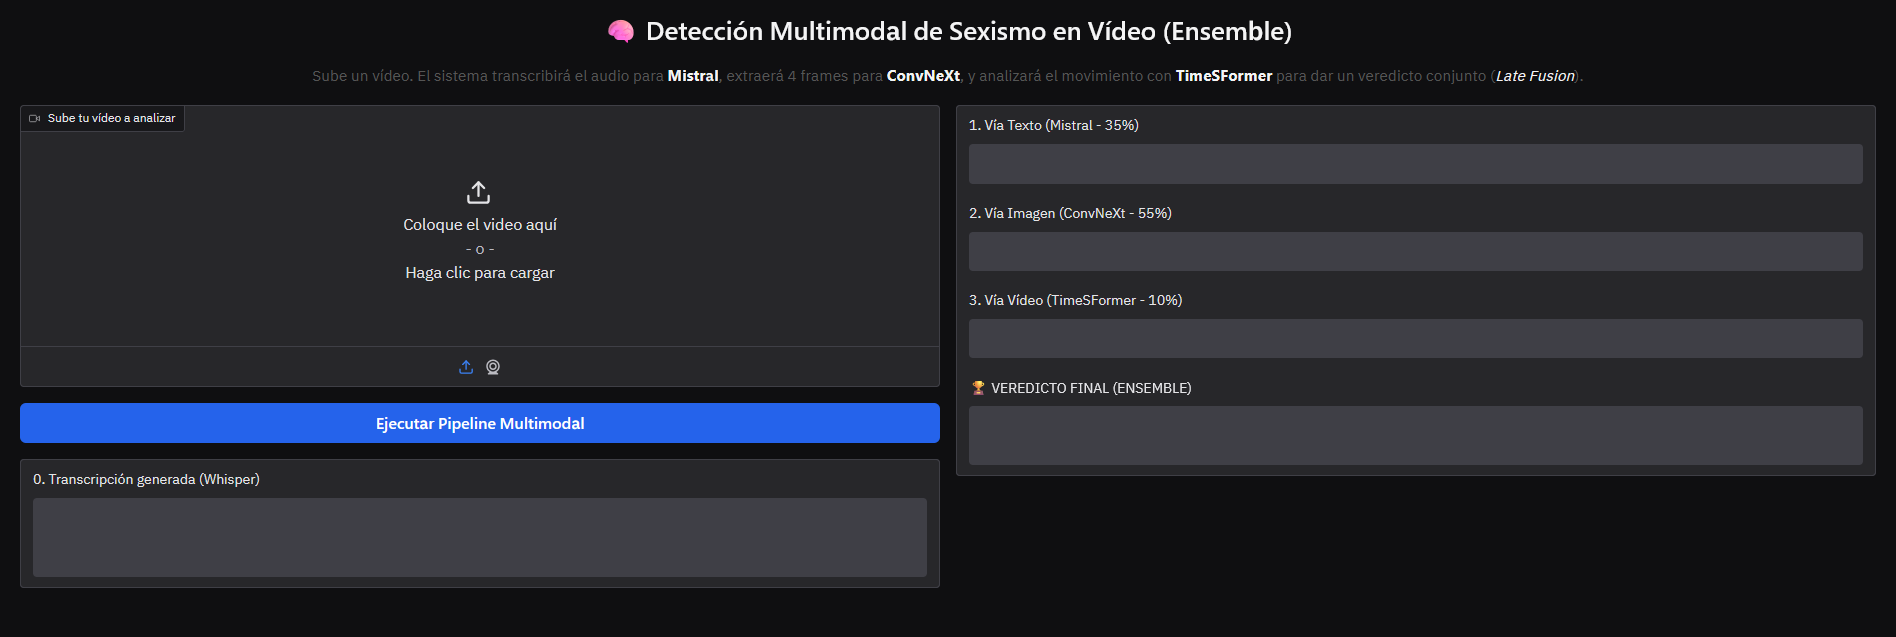
\includegraphics[width=1\textwidth]{Figuras/CapturaGradio.png}
    \caption{Interfaz web desarrollada con Gradio alojada mediante un \textit{iframe} en \textit{Hugging Face Spaces}.}
    \label{fig:CapturaGradio}
\end{figure}


\singlespacing

\end{document}
